\documentclass[12pt,a4paper,titlepage,listof=totoc,bibliography=totoc,chapteratlists=0pt]{scrreprt}

\begin{filecontents*}{\jobname.xmpdata}
	\Keywords{VR, IOT, TODO}
	\Title{Elektroauto Lademanager}
	\Author{Marcel Pouget, Teresa Holzer}
\end{filecontents*}

\setcounter{tocdepth}{1}

\usepackage[utf8]{inputenc}
\usepackage[T1]{fontenc}
\usepackage{amsmath}
\usepackage{amsfonts}
\usepackage{amssymb}
\usepackage[table]{xcolor}
\usepackage{graphicx}
\usepackage[left=3.50cm, right=2.00cm, top=2.00cm, bottom=2.00cm,foot=1cm]{geometry}
\usepackage[splitrule,hang,flushmargin,multiple,bottom]{footmisc}
\usepackage{lmodern, textcomp}
\usepackage{lmodern}
\usepackage{pdfpages}
\usepackage[ngerman]{babel}
\usepackage{multicol}
\usepackage{subfig}
\usepackage{float}
\usepackage{array,tabularx,booktabs}
\usepackage{ragged2e}
\usepackage{lipsum}
\usepackage{wrapfig}

\newcolumntype{M}[1]{>{\centering\arraybackslash}m{#1}}

\usepackage{enumitem}
\newlist{compactitem}{itemize}{3}
\setlist[compactitem,1]{label=\textbullet, nosep,leftmargin=1.5em,labelwidth=*,align=left}
\setlist[compactitem,2]{label=--, nosep,leftmargin=1.5em,labelwidth=*,align=left}
\setlist[compactitem,3]{label=\textopenbullet, nosep,leftmargin=1.5em,labelwidth=*,align=left}
\newlist{compactenum}{enumerate}{3}
\setlist[compactenum,1]{label=\arabic*., nosep,leftmargin=1.5em,labelwidth=*,align=left}
\setlist[compactenum,2]{label=\alph*., nosep,leftmargin=1.5em,labelwidth=*,align=left}
\setlist[compactenum,3]{label=\roman*., nosep,leftmargin=1.5em,labelwidth=*,align=left}
\newlist{compactdesc}{description}{3}
\setlist[compactdesc]{leftmargin=1.5em,labelwidth=*,align=left}

\usepackage{microtype}

\usepackage[parfill]{parskip}

\definecolor{bluekeywords}{rgb}{0.13,0.13,1}
\definecolor{greencomments}{rgb}{0,0.5,0}
\definecolor{redstrings}{rgb}{0.9,0,0}
\definecolor{lightgray}{gray}{0.9}
\definecolor{lightblue}{rgb}{0.93,0.95,1.0}

\usepackage{listings}

\makeatletter
\lstdefinestyle{lststyle}{
	basicstyle=%
	\ttfamily
	\lst@ifdisplaystyle\scriptsize\fi
}
\makeatother

\renewcommand{\lstlistlistingname}{List of Listings}
% TODO: define other languages as needed
\lstset{language=Python,
numbers=left,               
numberstyle=\tiny,          
showspaces=false,
showtabs=false,
breaklines=true,
lineskip=-1pt,
tabsize=2,
showstringspaces=false,
breakatwhitespace=true,
escapeinside={(*@}{@*)},
commentstyle=\color{greencomments},
keywordstyle=\color{bluekeywords}\bfseries,
stringstyle=\color{redstrings},
style=lststyle,
xleftmargin=17pt,
         framexleftmargin=17pt,
         framexrightmargin=5pt,
         framexbottommargin=4pt
}
\lstset{
morekeywords={base,var,in,out,dynamic,from,where,select,orderby,function,\$,group,by,into,yield,async,await,@,None,self,as,elif,with}
}
\lstdefinelanguage{TypeScript}{
	keywords={typeof, new, true, false, catch, function, return, null, switch, var, if, in, while, do, else, case, break, void, number, string, boolean, module, \$, export, for, this},
	keywordstyle=\color{blue}\bfseries,
	ndkeywords={class, export, boolean, throw, implements, import, this},
	ndkeywordstyle=\color{darkgray}\bfseries,
	identifierstyle=\color{black},
	sensitive=false,
	comment=[l]{//},
	morecomment=[s]{/*}{*/},
	commentstyle=\color{purple}\ttfamily,
	stringstyle=\color{red}\ttfamily,
	morestring=[b]',
	morestring=[b]"
}
\usepackage{caption}
\DeclareCaptionFont{white}{\color{white}}
\DeclareCaptionFormat{listing}{\colorbox[cmyk]{0.43, 0.35, 0.35,0.01}{\parbox{\textwidth}{\hspace{10pt}#1#2#3}}}
\captionsetup[lstlisting]{format=listing,labelfont=white,textfont=white} 
\captionsetup[table]{justification=centering, singlelinecheck=false}

\usepackage{setspace}
\newcommand{\MSonehalfspacing}{%
	\setstretch{1.44}%  default
	\ifcase \@ptsize \relax % 10pt
	\setstretch {1.448}%
	\or % 11pt
	\setstretch {1.399}%
	\or % 12pt
	\setstretch {1.433}%
	\fi
}

\newcommand{\setauthor}[1]{\ohead[]{#1}}

\usepackage[automark]{scrlayer-scrpage}
\pagestyle{scrheadings}
\automark{chapter}
\renewcommand\sectionmark[1]{\markright{\MakeMarkcase {\thesection\hskip .5em\relax#1}}}
\rohead{\ifnum\expandafter\pdfstrcmp\botmark=0 \rightmark\else\leftmark{} --- \rightmark\fi}
\ihead[]{\headmark}
\chead[]{}
\ohead{}
\cfoot[]{}
\ofoot[\pagemark]{\pagemark}
\setheadsepline{.1pt}

\usepackage[hyphens]{url}

\usepackage[a-1b]{pdfx}

\usepackage{hyperref}
\hypersetup{pdfa}

\usepackage[nonumberlist,toc,nopostdot]{glossaries}

\usepackage{chngcntr}
\counterwithout{footnote}{chapter}
\counterwithout{figure}{chapter}
\counterwithout{table}{chapter}
\AtBeginDocument{
	\counterwithout{lstlisting}{chapter}
	\urlstyle{sf}
}
\newcounter{RPages}

\makeatletter
\def\bstctlcite{\@ifnextchar[{\@bstctlcite}{\@bstctlcite[@auxout]}}
\def\@bstctlcite[#1]#2{\@bsphack
	\@for\@citeb:=#2\do{%
		\edef\@citeb{\expandafter\@firstofone\@citeb}%
		\if@filesw\immediate\write\csname #1\endcsname{\string\citation{\@citeb}}\fi}%
	\@esphack}
\makeatother

\clubpenalty=10000
\widowpenalty=10000
\displaywidowpenalty=10000
\interfootnotelinepenalty=10000

\title{Elektroauto Lademanager für die Firma
Flexsolution}
\author{Teresa Holzer, Marcel Pouget}

\makeindex
\makeglossaries
\begin{document}
\bstctlcite{IEEEexample:BSTcontrol}
\newcommand{\reminder}[1]
{ \textcolor{red}{<[{\bf\marginpar{\mbox{$<==$}} #1 }]>} }
\newcommand{\icode}[1]{\lstinline$#1$}
%\urlstyle{same}
%\setstretch{1.5}
\setstretch {1.433}
\renewcommand{\arraystretch}{1.2}

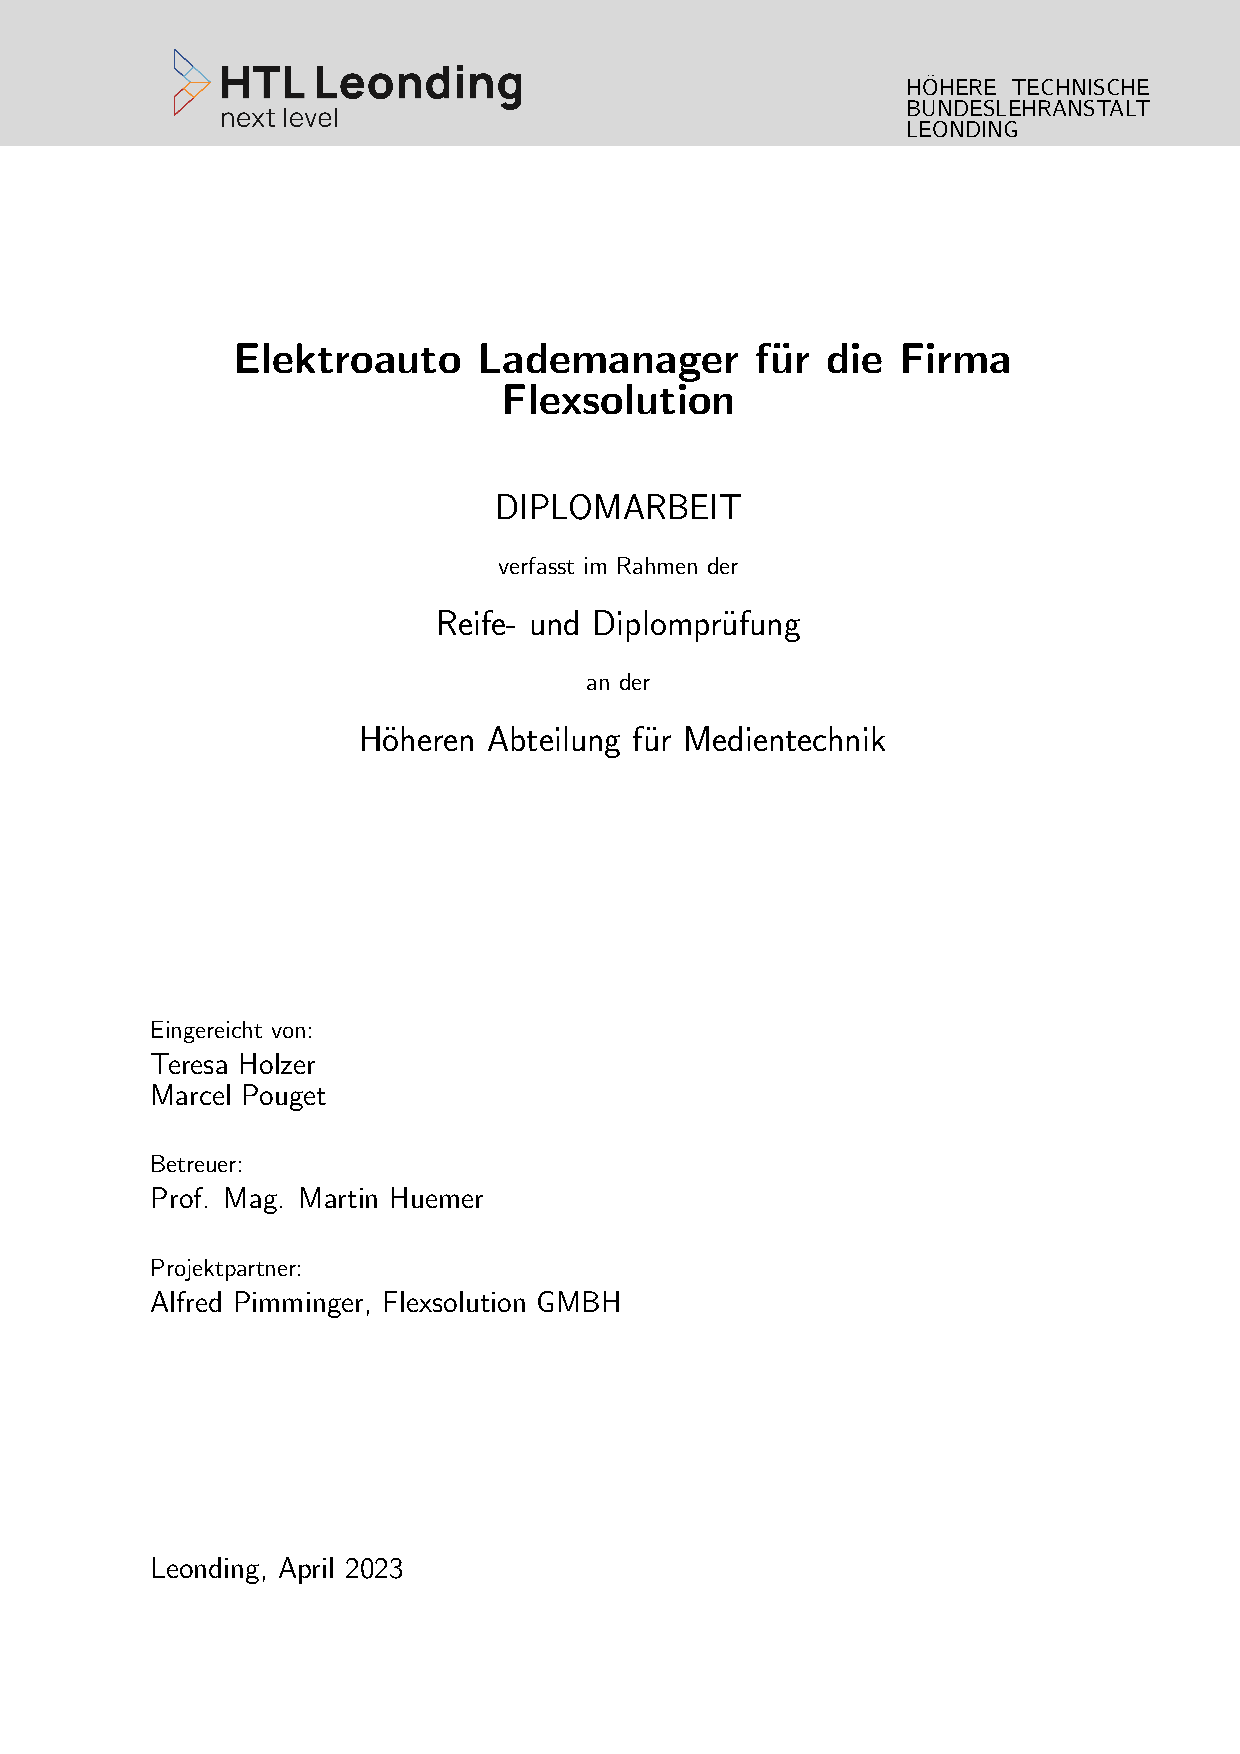
\includepdf{./titlepage/coversheet}
\pagenumbering{Roman}
\newpage
\thispagestyle{empty}
\vspace{3cm}
~ \\ \\
Ich erkläre an Eides statt, dass ich die vorliegende Diplomarbeit selbstständig und ohne fremde Hilfe verfasst, andere als die angegebenen Quellen und Hilfsmittel nicht benutzt bzw. die wörtlich oder sinngemäß entnommenen Stellen als solche kenntlich gemacht habe.

Die Arbeit wurde bisher in gleicher oder ähnlicher Weise keiner anderen Prüfungsbehörde vorgelegt und auch noch nicht veröffentlicht.

Die vorliegende Diplomarbeit ist mit dem elektronisch übermittelten Textdokument identisch.
\vspace{3cm}
% Hier kommt die Unterschrift drüber
\begin{tabbing}
Leonding, April 2022 \hspace{5cm} T. Holzer \& M. Pouget
\end{tabbing}
\vspace{10cm}
\newpage
\setcounter{page}{1}

\begin{spacing}{1}
    \chapter*{Abstract}
\end{spacing}
\begin{wrapfigure}{r}{0.3\textwidth}
    \begin{center}
      
\includegraphics[width=0.2\textwidth]{pics/question_mark.png}
    \end{center}
\end{wrapfigure}
This is the description of the journey to succeed this project.
It took way longer than I thought, it was a lot of work and struggled, 
but in the end we did it. And if you are reading this right now it means,
that everything went exactly as planned. And this is great, because it means
 that I have my A-Levels done, and don’t have to go to this shitty school. Don’t worry, I will correct this summary, but right now I don’t know what's important, so I write just what comes in my mind. Enjoy it, and pls write me, if you find some mistakes: smalldickenergy@grethat.tu” 
\newpage
\begin{spacing}{1}
    \chapter*{Zusammenfassung}
\end{spacing}
\begin{wrapfigure}{r}{0.3\textwidth}
    \begin{center}
      
\includegraphics[width=0.2\textwidth]{pics/question_mark.png}
    \end{center}
\end{wrapfigure}
Zusammenfassung unserer genialen Arbeit. Auf Deutsch.
Das ist das einzige Mal, dass eine Grafik in den Textfluss eingebunden wird.
Die gewählte Grafik soll irgendwie eure Arbeit repräsentieren.
Das ist ungewöhnlich für eine wissenschaftliche Arbeit aber eine Anforderung der Obrigkeit.
\emph{Bitte auf keinen Fall mit der Zusammenfassung verwechseln, die den Abschluss der Arbeit bildet!}



\pagestyle{plain}

\renewcommand{\lstlistlistingname}{Quellcodeverzeichnis}

\tableofcontents
\newpage
\setcounter{RPages}{\value{page}}
\setcounter{page}{0}
\pagenumbering{arabic}
\pagestyle{scrheadings}

\begin{spacing}{1}
\chapter{Einleitung}\label{chapter:introduction}
\end{spacing}
\setauthor{Marcel Pouget}
Die Arbeit wurde zusammen mit der Firma FlexSolution GmbH entwickelt. Diese stellten auch die benötigte Hardware in Form von Raspberrys, den Ladestationen und Arbeitsplätzen zur Verfügung. Bei Problemen standen zwei Mitarbeiter immer zu Verfügung und halfen mit, Probleme zu lösen. Die Basis der Arbeit wurde schon in einem Ferialpraktikum im Sommer 2021 gelegt, in welchem mit Zusammenarbeit qualifizierter Fachkräfte die Ladestationen montiert wurden. Der programmierende Anteil des Projektes wurde im Zuge eines Praktikums im Jahre 2022 umgesetzt. Dieses dauerte 4 Wochen und war nur für die Entwicklung der Arbeit gedacht.


Die Idee eines Lademanagers entstand im Frühjahr 2021, als die Photovoltaikanlage der Firma fertiggestellt wurde. Marcel war zu dieser Zeit als Werksstudent bei der Firma angestellt und bekam das Angebot, dieses Projekt als Diplomarbeit umzusetzen. Da dieses Projekt alleine nicht den geforderten Umfang besaß, wurde zusammen mit dem Herrn Pimminger an einem zweiten Projekt, dem sogenannten Flexlogger getüftelt. Nach der Planungsphase gab es dann auch für diesen Teil des Projektes das 'Ok'


\section{Herangehensweise}


Nach einem ersten Briefing mit Alfred Pimminger wurden erste Pläne für das Projekt ausgearbeitet. Vor allem der Aufbau und das Zusammenspiel mit den firmeninternen Systemen war dabei äußerst wichtig. Die erste Skizze des Projektes sah dabei wie folgt aus:
\ref{fig:impl:ersteSkizze}


\begin{figure}[h t]
\centering
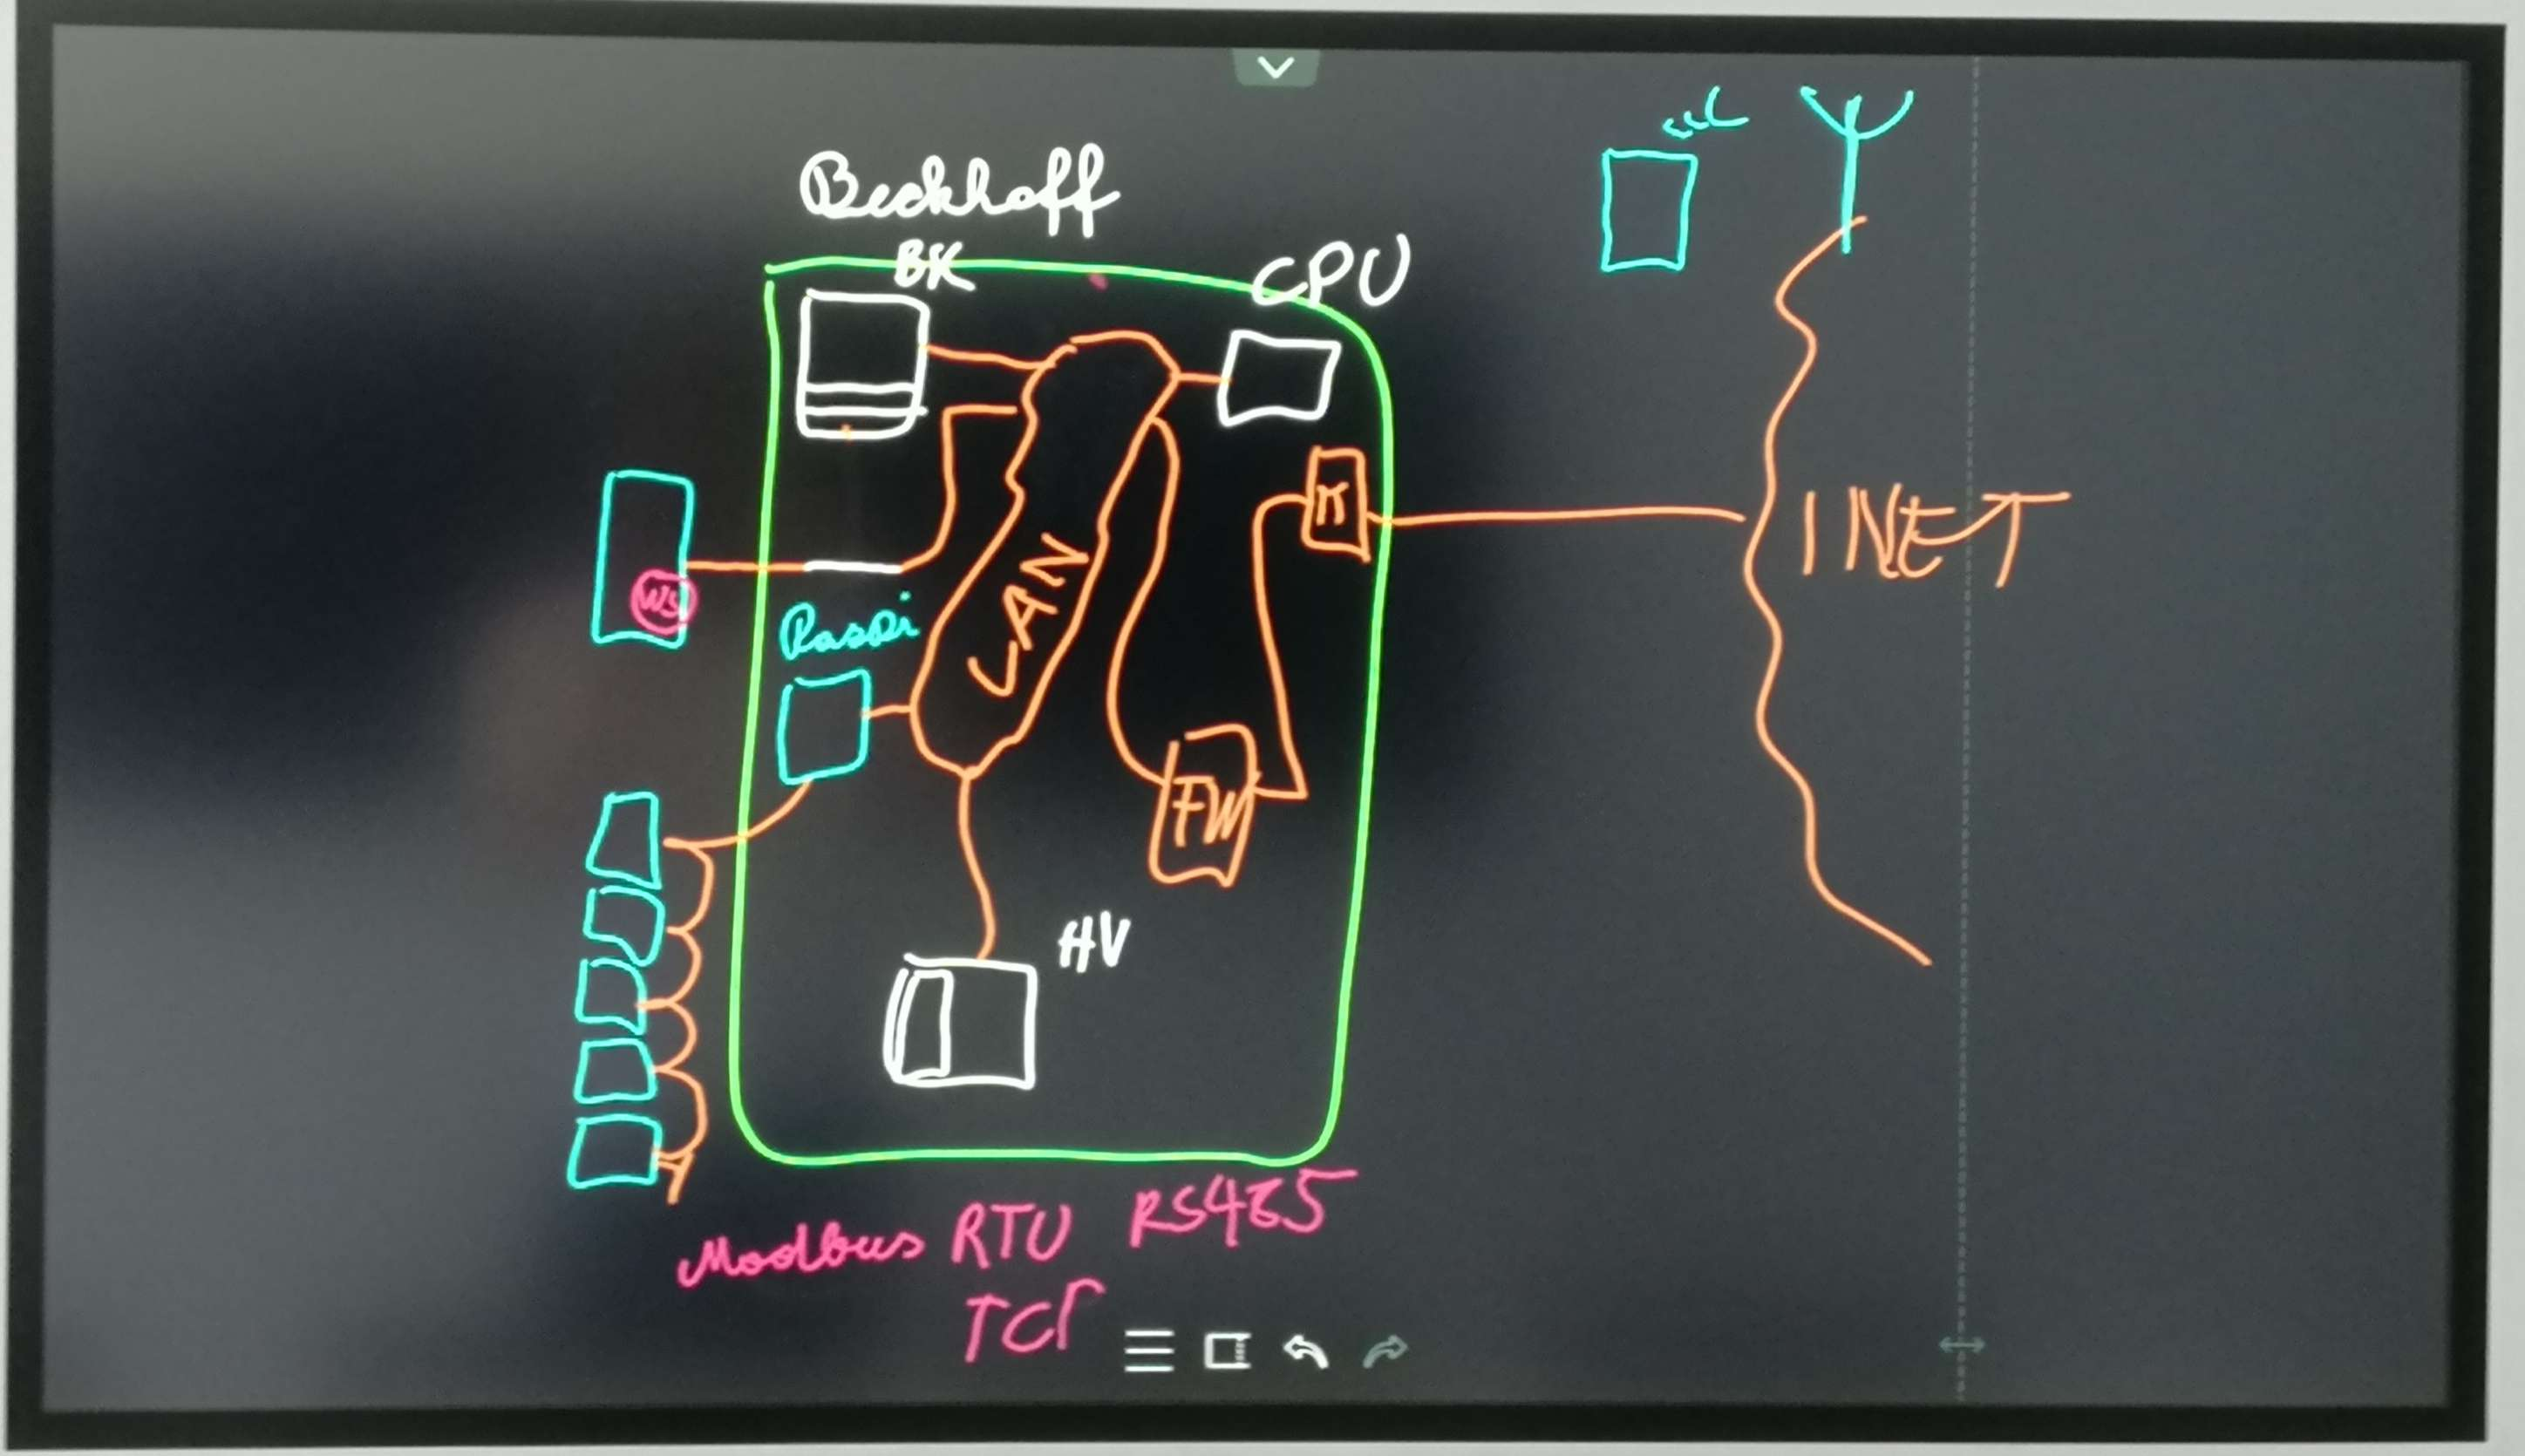
\includegraphics[scale=0.15]{pics/ersteSkizze.jpg}
\caption{Erste Planung auf einem Whiteboard}
\label{fig:impl:ersteSkizze}
\end{figure}



Der Aufbau hat sich im Laufe der Entwicklung leicht verändert, jedoch blieb die Grundbasis erhalten, siehe \ref. {section:aufbaudesProjektesFlexlogger}. Das Projekt über einen Logger entstand erst etwas später. Auch hier wurde der Aufbau der Arbeit während eines Meetings mit Alfred besprochen, jedoch geschah die Umsetzung erst einige Monate später. Hier war der Plan, von verschiedensten Flextasks die Daten zu speichern, da diese bis jetzt immer gelöscht wurden. Die Planung für den Aufbau des Projektes geschah erst im Zuge der Entwicklung, siehe \ref{AufbauDesProjektesWallbox}
\setauthor{Marcel Pouget}



\section{Zeitplan}
\setauthor{Marcel Pouget | Teresa Holzer}



Um das Projekt problemlos umsetzen zu können, wurden noch vor dem eigentlichen Projektstart zehn Meilensteine angelegt.


\begin{compactitem}
\item 30.06.2022 Fertigstellung Pflichtenheft
\item 07.08.2022 Datenbank aufsetzen (Flexlogger)
\item 07.08.2022 Flexlogger Server aufsetzen (Flexlogger)
\item 07.08.2022 Task für Kommunikation mit den Wallboxen aufsetzen (Wallboxen)
\item 14.08.2022 Geloggte Daten kommen bei dem Frontend an (Flexlogger)
\item 14.08.2022 Task für das Steuern der Wallboxen aufsetzen (Wallboxen)
\item 21.08.2022 Daten werden visualisiert (Flexlogger)
\item 21.08.2022 Die Verbindung zwischen UI und den Wallboxen steht (Wallboxen)
\item 31.08.2022 Fertigstellung der Website für die Wallboxen (Wallboxen)
\item 31.08.2022 Fertigstellung des Flexloggers (Flexlogger)
\end{compactitem}


\section{Verwendete Tools}
Während der Entwicklung des Projektes wurden viele verschiedene Systeme verwendet, um den Verlauf des Projektes zu beschreiben. Welche dieser Tools in Verwendung waren und wie sie eingesetzt wurden, wird in diesem Kapitel beschrieben.



\subsection{Latex [M]} \setauthor{Marcel Pouget}


Latex ist eine Software, welche es ermöglicht, Texte, Graphiken und Bilder zu layoutieren und zu exportieren. Sie basiert auf dem Textsatzsystem TeX und arbeitet nach der Methode WYSIWYM (What You See Is What You Mean). Das heißt, dass der Text, welcher im Endprodukt angezeigt werden soll, in einem Quelldokument erstellt wird und erst nach dem Kompelieren eine Formatierung enthält. Das ermöglicht es schnell Verweise zu anderen Textstellen zu integrieren, eine automatische Beschriftung für Bilder und Quellen, ein Literaturverzeichnis, welches einen guten Überblick bietet. Natürlich darf ein automatisch-generiertes Inhaltsverzeichnis nicht fehlen, welches mit Verschieben der Komponenten aktualisiert werden kann. Das ermöglicht es, ganze Kapitel innerhalb von Sekunden neu zu strukturieren, ohne dass Beschriftungen oder andere Layouts ihre Gültigkeit verlieren. Ein paar weitere Vorteile von Latex sind:


\begin{compactitem}
\item Die Qualität der Dokumente ist sehr hoch.
\item Die Dokumente werden automatisch klar und einheitlich formatiert. Da dies bei wissenschaftlichen Arbeiten immer eine Voraussetzung ist, ist Latex oft die richtige Wahl.
\item Es können mathematische Formeln, Codebeispiele, Tabellen, Bilder und vieles mehr ohne Probleme mit der Formatierung eingebettet werden.
\item Die Ausgangstexte sind plain Text, das heißt, es kann sowohl von jedem gelesen, verstanden als auch bearbeitet werden.
\item Da größere Arbeiten immer aus mehreren Dokumenten bestehen, ist Latex sehr flexibel. Es ist möglich, die Struktur mit Ordnern beliebig zu wechseln, Einstellungen für eine gewisse Anzahl an Seiten oder für das ganze Dokument zu treffen. Dadurch eignet es sich sehr gut für Projekte, an denen mehrere Autoren gleichzeitig arbeiten.
\item Latex ist opensource, und sehr gut dokumentiert. Es gibt viele Anleitungen dazu, es kann benützt werden und es wird von jedem gängigen Betriebssystem unterstützt.
\item Außerdem gibt es für verschiedene Anwendungszwecke vorgefertigte Templates, welche das Arbeiten erleichtern. In solchen gibt es schon eine globale Einstellung für Schrift, Absätze, Nummerierungen und Deckblätter. Dies erleichtert die Arbeit sehr, da nicht immer von vorne beginnen werden muss, wenn ein neues Dokument erstellt werden möchte.
\end{compactitem}


Diese Punkte ermöglichen es dem Autor*in, sich nicht auf das Layout konzentrieren zu müssen, sondern ermöglichen es, sich nur auf den Inhalt zu fokussieren. Der Rest wird voll und ganz von der installierten Software übernommen.




Ein Latex-Projekt kann in jedem Beliebigen Editor gestartet werden. Wichtig dabei ist nur, dass das Programm Latex an sich auf dem Rechner installiert wurde und alle Abhängigkeiten automatisch heruntergeladen wurden. Editoren wie Visual Studio Code unterstützen eigene Plugins für Latex, in welchem das ganze Projekt übersichtlich an der Seite angezeigt wird. Dies bietet den Vorteil, dass nicht nur eine Live-Vorschau ermöglicht wird, sondern auch die Navigation in komplexen Projekten vereinfacht wird.




Ein neues Projekt wird angelegt, indem eine \grq.tex\grq Datei erstellt wird. In dieser kann dann schon reiner Text geschrieben werden, jedoch wird das Layout noch nicht die gewünschte Form bekommen.


Um das zu erreichen, gibt es die Möglichkeiten von sogenannten Templates, welche oft von Firmen, Universitäten oder Schulen angeboten werden (siehe z. B. das Latex-Template: \url{https://github.com/markushaslinger/latex_htl_da_template}). In solchen vorgefertigten Projekten gibt es schon eine klare Struktur und Files, welche sich um das Layoutieren kümmern. Vorteil davon ist, dass sehr viel Arbeit von Latex übernommen wird und der Fokus rein auf den Inhalt gelegt werden kann.
\cite{latexHeise}
\cite{LatexUniGraz}
\cite{LatexUni}


\subsection{Intellij [M]} \setauthor{Marcel Pouget}


Intellij ist eine IDE (Integrated Development Environment, oder zu Deutsch: Integrierte Entwicklungsumgebung), welche für die Entwicklung in Java und Kotlin optimiert ist. Das Programm bietet eine Vielzahl an Hilfsmitteln und Plugins, um das Entwickeln zu vereinfachen. Von intelligenter Code-completion bis zu intuitiven Debugging Möglichkeiten ist alles dabei. Und sollte eine Sprache oder ein Feature nicht unterstützt werden, sind im Plugin-Store noch unzählige Anpassungen, welche die IDE noch besser machen. Ein großer Bestandteil der Software ist die Möglichkeit, Build-Tools wie Maven oder Gradle von Haus aus zu verwenden. Ein Beispiel ist bei \ref{fig:impl:WallboxMavenTap} zu sehen. Außerdem ist es möglich, ohne Windows / Linux Umgebungsvariablen den Code direkt in der Applikation zu testen. Dafür wird die ausgewählte JDK heruntergeladen und so konfiguriert, dass zuverlässig jeder Code mit einem Click gestartet werden kann. Sollten Dependencies fehlen, ist es möglich, sie mit einer integrierten Suche hinzuzufügen und mit einem eigenen Tap für Maven herunterzuladen.


\begin{figure}[h t]
\centering
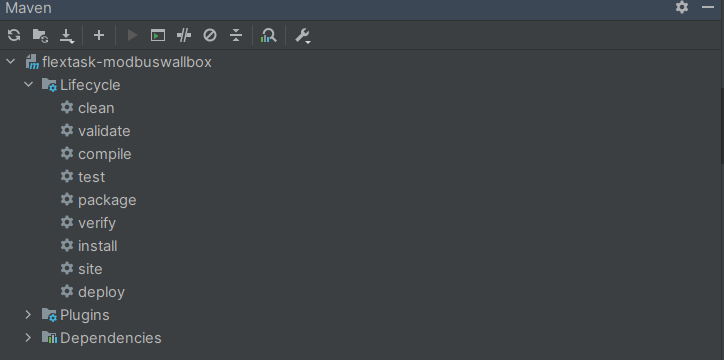
\includegraphics[scale=0.55]{pics/MavenOverfiew.png}
\caption{So sieht der Maven-Tap in Intellij aus}
\label{fig:impl:WallboxMavenTap}
\end{figure}


Die Ordnerübersicht und die Möglichkeit, Variablen in einem ganzen Projekt zu refactoren, sind unterstützend, wenn es um Änderungen in den eigenen Projekten geht. Eine globale Suche und eine Formatierungsfunktion helfen dabei, die User Experience zu erhöhen. Die Intellij IDE kann in zwei Produkte unterteilt werden: die kostenlose Opensource-Kommunikation-Edition und die kostenpflichtige Ultimate-Version. Während die kostenlose Version eine gute Möglichkeit ist, schnell kleinere Programme umzusetzen, ist vor allem Ultimate besser geeignet, große Projekte mit mehreren Mitarbeitern zu bewältigen. Dafür ist selbstverständlich ein Versionscontrol-System integriert, welches sich problemlos mit Anbietern wie z.B. Github nutzen lässt.


\begin{figure}[h t]
\centering
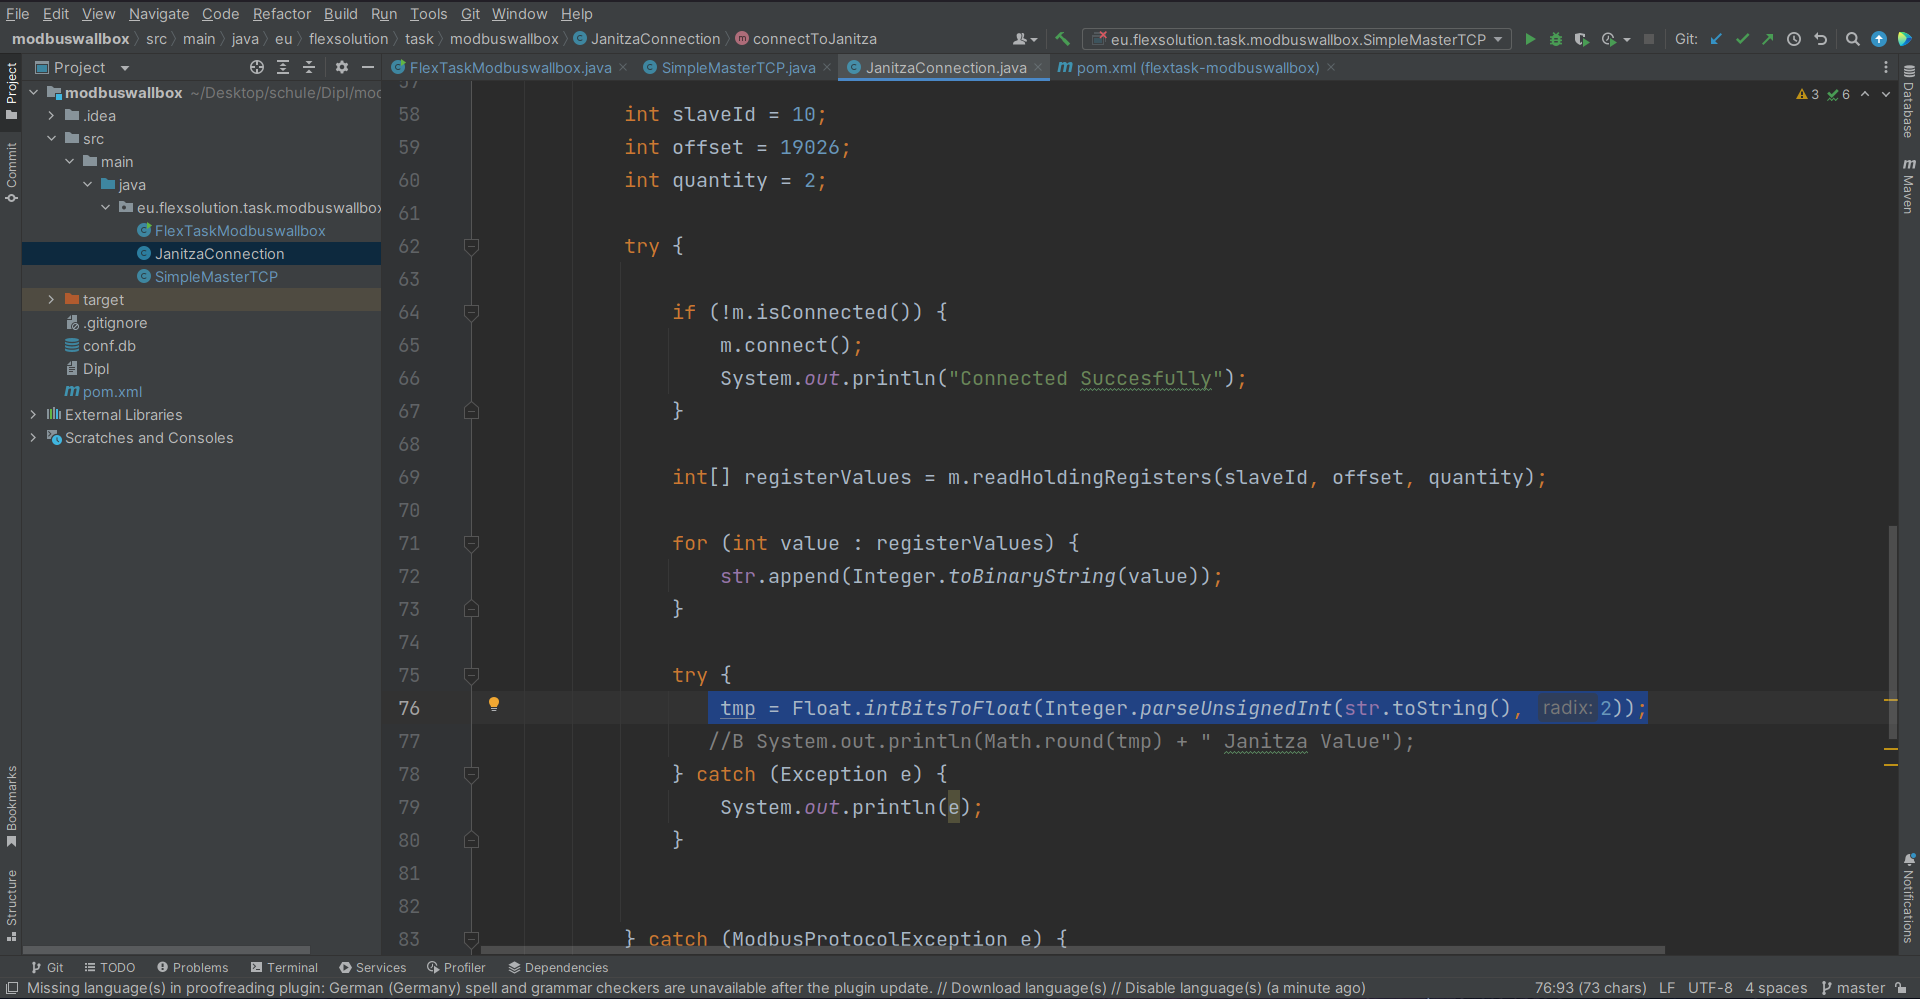
\includegraphics[scale=0.2]{pics/IntellijOverfiew.png}
\caption{Ansicht von einem Intellij Projekt}
\label{fig:impl:WallboxIntellij}
\end{figure}


Und auch wenn IntelliJ IDEA in erster Linie für die Java- und Kotlin-Entwicklung vorgesehen wurde, unterstützt die IDE auch viele weitere gängige Programmiersprachen wie Groovy, Javascript, Typescript und SQL. Für letzteres gibt es sogar einen eigenen Tab, in welchem ohne Probleme eine Datenbankverbindungen aufgebaut und getestet werden können. Ein kleiner Überblick über die einzelnen Tabs und sogar eine Konsole für SQL-Querrys sind auch geboten.


\cite{IntellijJetbrains}





\subsection{Webstorm [T]} \setauthor{Teresa Holzer}
% < https://www.jetbrains.com/de-de/webstorm/
\setauthor{Teresa Holzer [T]}\setauthor{Teresa Holzer}
WebStorm, Interface siehe Abb. \ref{fig:impl:webstorm}, wird als Entwicklungsumgebung für JavaScript und JavaScript-ähnliche Sprachen definiert. Es ist außerdem geeignet für die Entwicklung mit Angular, da ein neues Projekt direkt in WebStorm erstellt und in der Entwicklungsumgebung gestartet werden kann. WebStrom wurde, genau wie IntelliJ, von JetBrains entwickelt und liefert eine Reihe von Hilfestellungen, um JavaScript optimal programmieren zu können. WebStorm beinhaltet eine automatische Code-Überprüfung sowie die automatische Komplettierung von einzelnen Codezeilen. WebStorm beinhaltet außerdem einen bereits eingebauten Run- sowie Debug-Button, durch welchen das Starten in der Konsole wegfällt. Zusätzlich können in WebStorm verschiedenste Plugins hinzugefügt werden, welche das Erscheinungsbild verändern, andere Sprachen überprüfen können und vieles mehr. \cite{webstormOfficialSite}


\begin{figure}[h t]
\centering
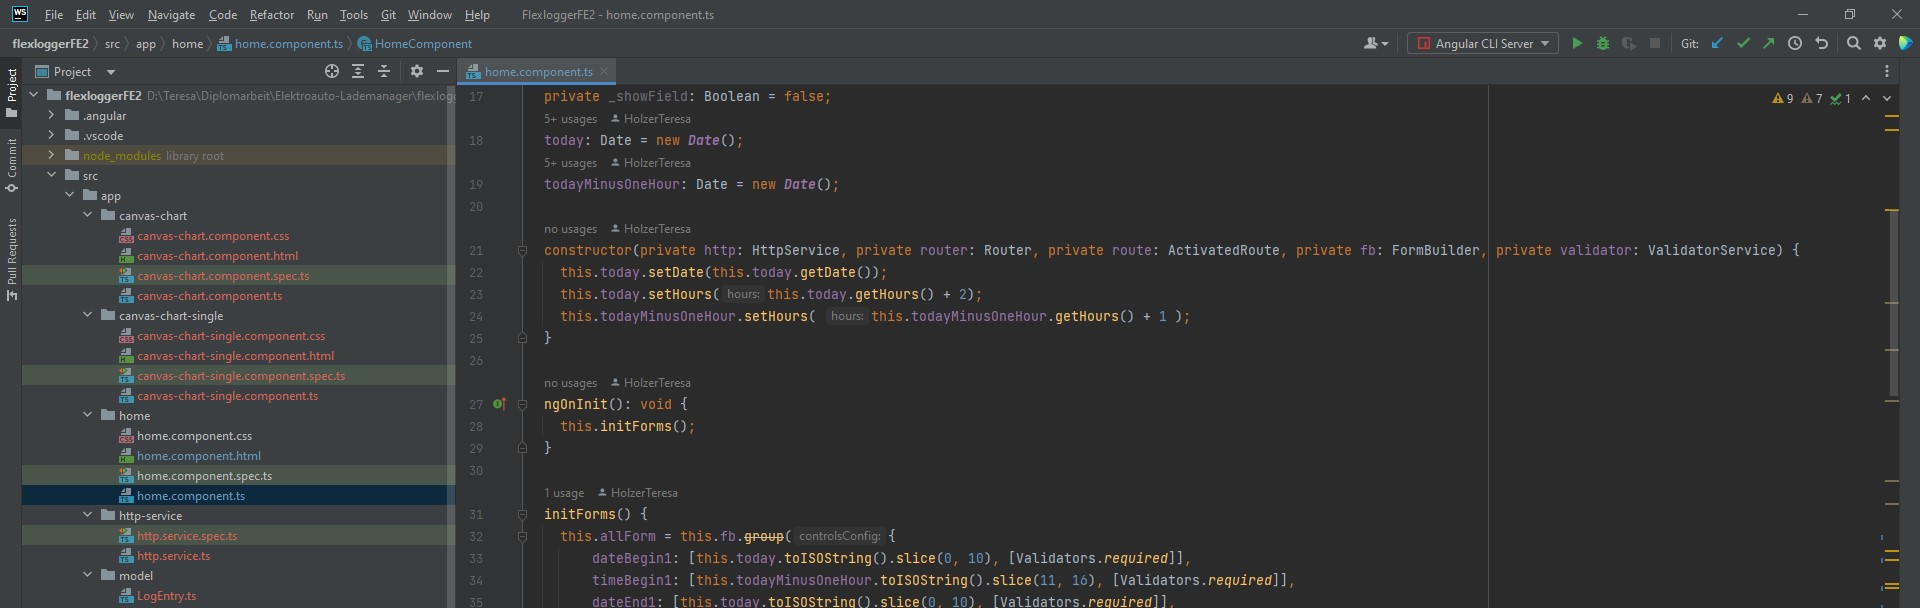
\includegraphics[scale=0.38]{pics/webstorm.jpg}
\caption{WebStorm}
\label{fig:impl:webstorm}
\end{figure}



\subsection{Linux Terminal [M]} \setauthor{Marcel Pouget}
Vieles der Entwicklung fand in der Kommandozeile von Linux statt. Von der Überwachung des Status der Tasks bis hin zum Starten der App lief alles in einem Terminal ab. Dabei handelt es sich um ein Programm, welches einen Text von einem User*in entgegennimmt und als Befehl interpretiert. Dadurch lassen sich Verbindungen zu weiteren Geräten via SSH ermöglichen, um aus der Ferne Projekte zu entwickeln. So kann der Raspberry Pi4 in einem Schaltschrank der Firma montiert sein und trotzdem kann ein Entwickler aus dem Büro die Einstellungen verändern.


Mit einer sogenannten CLI (Command Line Interface) lassen sich Programme ohne graphische Useroberfläche bedienen, Ordner und Files verwalten und ganze Serverstrukturen verwalten.


\cite{CommandolineFortext}


\subsection{Discord [M]} \setauthor{Marcel Pouget}
Discord ist eine kostenlose App für Kommunikation via Sprache, Chat und Video. Dies ermöglicht einen schnellen, reibungslosen Austausch zwischen einzelnen Personen bis hin zu großen Gruppen. Im Zusammenhang dieser Arbeit wurde die Applikation dafür benutzt, um Aufgaben zu verteilen, Informationen auszutauschen und Meetings zu halten. Ein Server für dieses Projekt wurde erstellt, um immer einen Überblick der aktuellen Dokumente zu bekommen. Auch die Links zu Informationen, Terminen und dem Google Drive-Laufwerk wurden gespeichert.


Discord half vor allem bei der Organisation unter den Projektmitgliedern. Dadurch konnte eine reibungslose Kommunikation gewährleistet werden.


\cite{discordEpic}
\subsection{Google drive [T]} \setauthor{Teresa Holzer}


% < https://one.google.com/about
Google Drive ist ein Cloud-Speicher, welcher für das Online-Speichern von Google Docs, Google Tabellen, Google Präsentationen und Google Formularen verwendet werden kann. Außerdem können Bild- und andere Formate hochgeladen und somit gesichert werden. Google Drive kann kostenlos durch das Erstellen eines Google-Accounts verwendet werden. Google stellt dabei 15GB Speicher frei zur Verfügung, danach kann durch ein monatliches Abo-Modell mehr Speicherplatz erlangt werden. \cite{OneDriveOfficialSite}


Google Drive wurde im Rahmen dieser Diplomarbeit genutzt, um Dokumente und Dateien für alle Projektmitglieder leicht zugänglich zu machen.


\subsection{Visual Studio Code [T]} \setauthor{Teresa Holzer}
% < https://code.visualstudio.com/docs
Visual Studio Code, Interface siehe Abb. \ref{fig:impl:vsCode}, ist ein leistungsstarker Code Editor. Es ist verfügbar für Windows, Linux und macOS.
Einer der größten Vorteile von VS Code ist ein eingebautes Support-Tool für JavaScript, TypeScript und Node.js. Außerdem verfügt es über zahllose Erweiterungen für andere Programmiersprachen. VS Code besitzt auch einen Run und Debug Modus, um Programme direkt in der Umgebung ausführen zu können.
VS Code kann vielfältig eingesetzt werden und aufgrund der Erweiterungen nach Belieben personalisiert werden. \cite{VSCodeOfficialSite}


Um nur ein paar der Erweiterungen zu nennen, welche VS Code wandelbar machen:


\begin{compactitem}
\item Microsoft Visual Studio Live Share: Mithilfe dieser Extension ist es möglich, gleichzeitig von mehreren Computern an einem Projekt zu arbeiten.
\item C, C++, Python, ... : Durch diese Extensions kann leichter in der jeweiligen Programmiersprache programmiert werden, da IntelliSense und Debugging features hinzugefügt werden.
\item Visual Studio Code Remote – SSH: Mittels dieser Extension kann jeder entfernte Rechner mit einem SSH-Server als Entwicklungsumgebung verwendet werden.
\end{compactitem}
\cite{VSCodeOfficialSite}


Zur einfachen Ansicht von Code sowie zum Verfassen des schriftlichen Teils der Diplomarbeit mithilfe von Latex wurde VS Code verwendet.


\begin{figure}[h t]
\centering
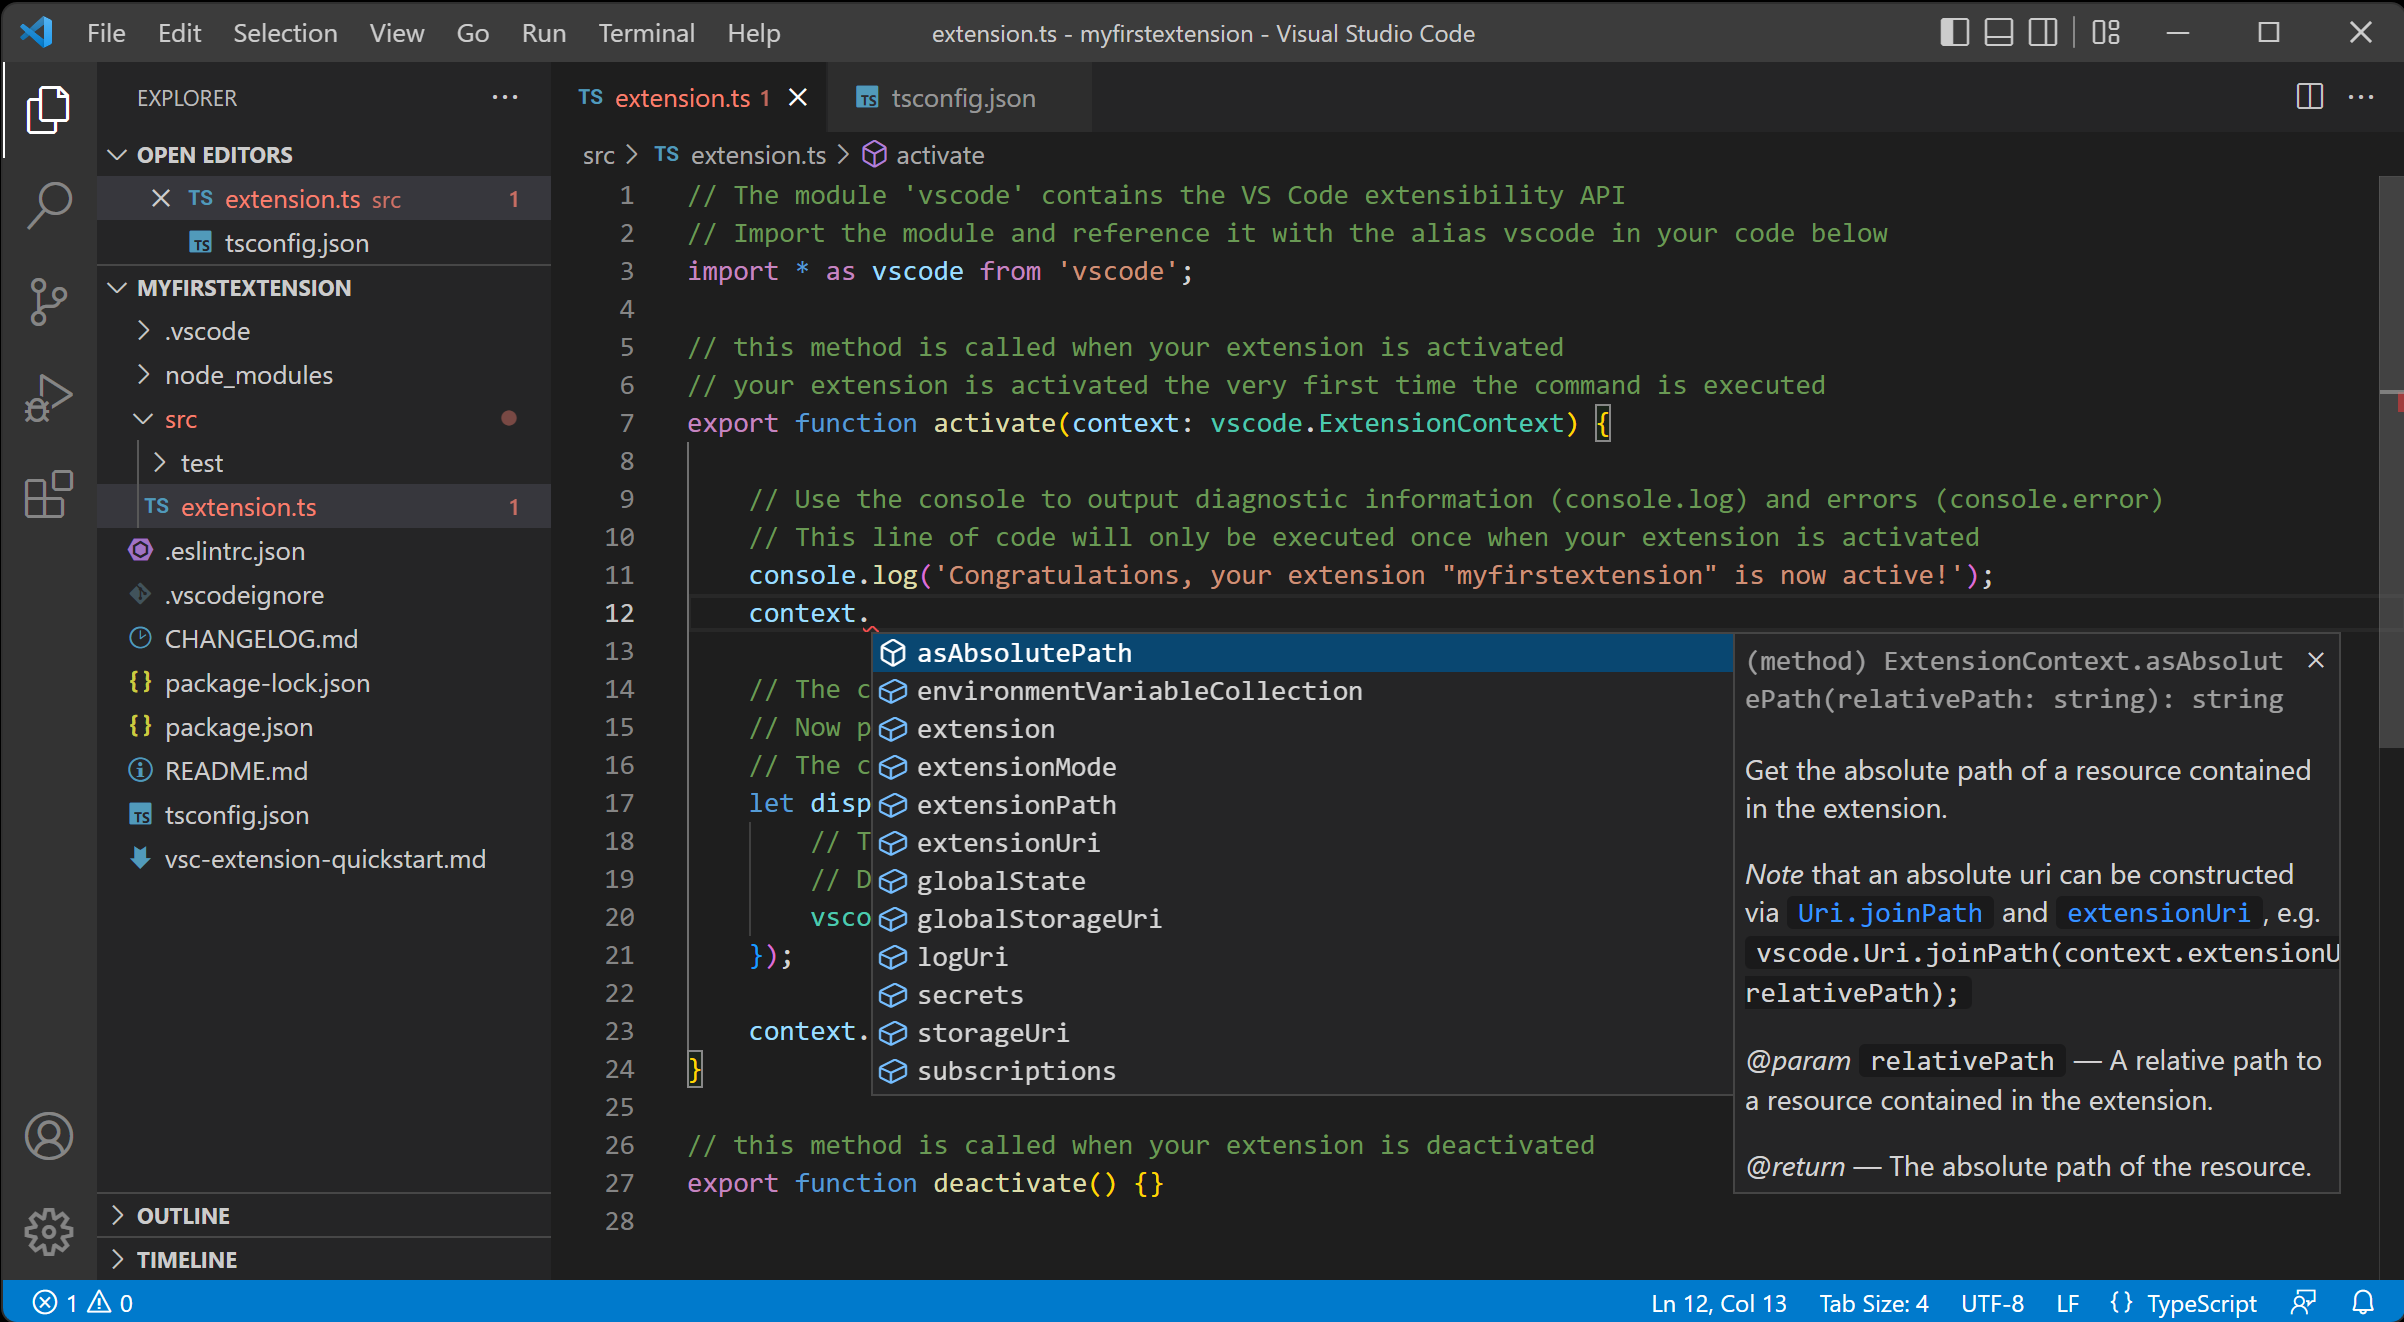
\includegraphics[scale=0.48]{pics/visualStudioCode.png}
\caption{Ansicht Visual Studio Code}
\label{fig:impl:vsCode}
\end{figure}


\subsection{Github [T]} \setauthor{Teresa Holzer}
% < https://github.com/features
GitHub ist ein Online-Tool, welches es ermöglicht, zusammen mit Teammitgliedern an Projekten zusammenzuarbeiten. Projekte können dabei mühelos neu heruntergeladen werden, es kann auf neue Versionen aktualisiert werden und es können Versionen mit verschiedenen Versionsnummern zusammengefügt werden. GitHub kann über das Terminal oder den GitHub Desktop verwendet werden, siehe Abb. \ref{fig:impl:gitHubTerminalVSGUI}.


\begin{figure}[h t]
\centering
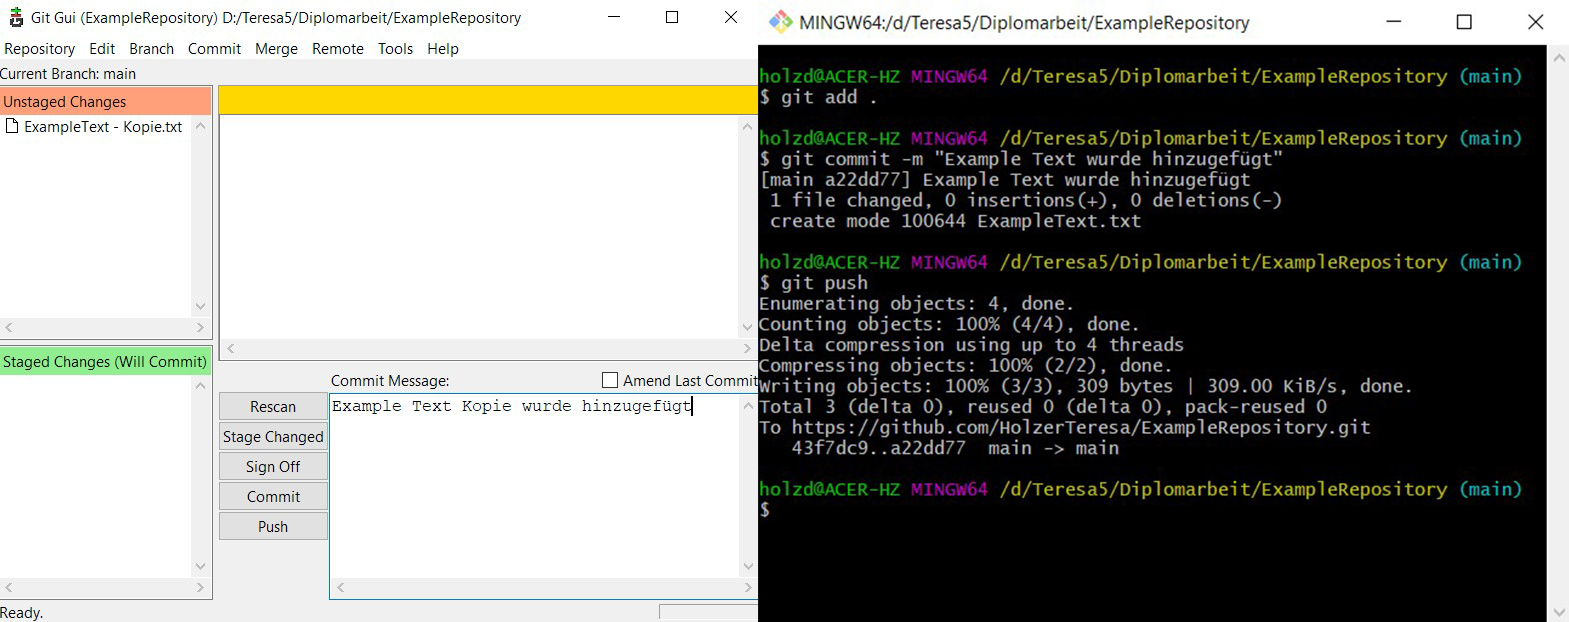
\includegraphics[scale=0.45]{pics/githubTerminalGUI.png}
\caption{GitHub Desktop vs. Terminal}
\label{fig:impl:gitHubTerminalVSGUI}
\end{figure}


Bei der Verwendung von GitHub können sogenannte Repositories, siehe Abb. \ref{fig:impl:githubRepository}, erstellt werden. In diese können neue Dokumente bzw. Dateien hinzugefügt werden. Ein Repository besitzt zusätzlich eine Beschreibung sowie eine Übersicht der Historie der hinzugefügten Dateien. Mithilfe dieser können vorherige Versionen wiederhergestellt bzw. gesichtet werden. Wenn also zum Beispiel die aktuelle Version eines Programms auf Discord einen Fehler enthält, kann ohne Probleme zu der vorherigen Version gewechselt werden.




\begin{figure}[h t]
\centering
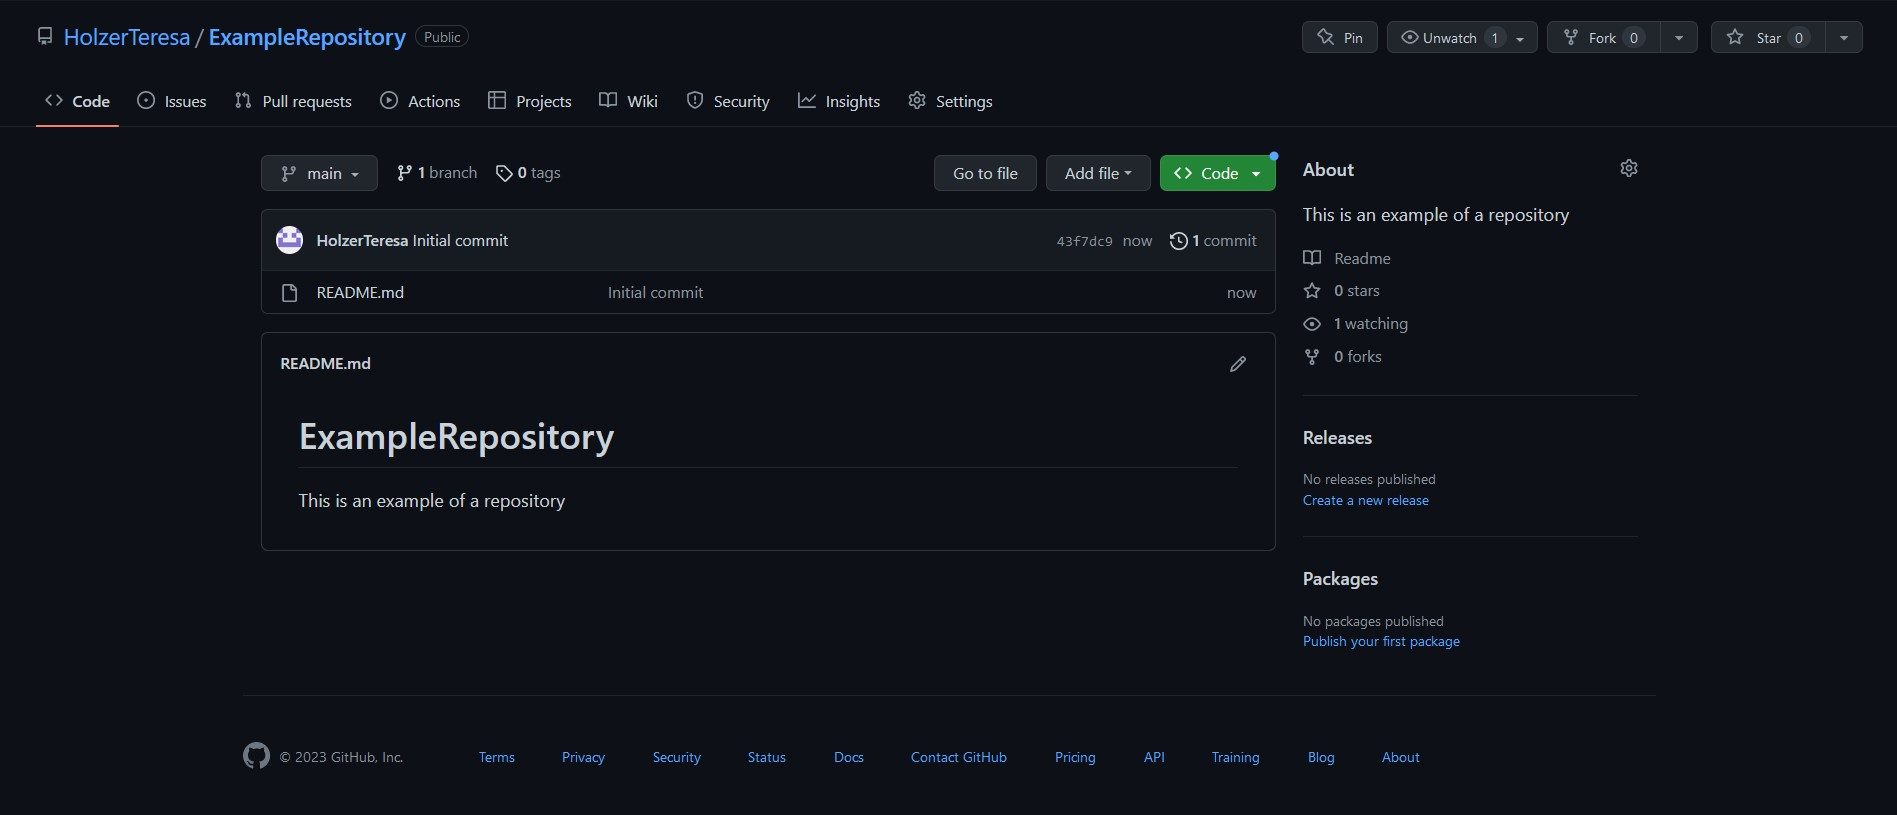
\includegraphics[scale=0.38]{pics/exampleRepository.jpg}
\caption{Beispiel eines GitHub-Repo}
\label{fig:impl:githubRepository}
\end{figure}



\begin{spacing}{1}
\chapter{Allgemeiner Technologie-Part}
\end{spacing}


\begin{spacing}{1}
    \setauthor{Pouget Marcel}
    \section{Java [M]}\label{section:allTechJava}
    \end{spacing}
Java ist eine kostenlose objektorientierte Programmiersprache, welche im Jahr 1995 von dem Unternehmen Sun Microsystems veröffentlicht wurde. Das Unternehmen Oracle kaufte im Jahr 2010 das Unternehmen und entwickelt seitdem die Sprache kontinuierlich weiter. Die Sprache ist neben C eine der bekanntesten Programmiersprachen weltweit. Sie kann auf allen bekannten Systemen installiert werden und garantiert durch den Aufbau, dass es auf jedem System lauffähig ist. Um das zu ermöglichen, setzt Java auf eine virtuelle Laufzeitumgebung (Java VM), auf welcher der Code ausgeführt wird. Das Java Development Kit (JDK) ist dabei ein wichtiger Bestandteil, denn der integrierte Compiler übersetzt den menschlichen Code in Maschinencode. 

Doch was ist der Vorteil einer sogenannten objektorientierten Sprache? Ganz einfach, es ermöglicht bei der Entwicklung, große Teile des Codes wieder zu verwenden. Das Ganze ist in Klassen und Objekte eingeteilt. Vergleichbar ist es mit einer Bauanleitung. So kann eine Klasse z.B. eine Anleitung für ein Auto sein mit Attributen wie Rädern, PS, Farbe und einem Baujahr. Sollten nun mehrere Autos gebraucht werden, können Objekte vom Typ Auto erstellt werden. Dabei hat jedes Auto dieselben Variablen, aber unterschiedliche Werte. Es können auch Funktionen aus der Klasse benutzt werden.  

Dies bietet die Möglichkeit, eine Vielzahl von Code zu recyclen. Ein weiterer wichtiger Punkt in Java sind die sogenannten Build Tools, die es erlauben, Librarys und Dependencies zu dem Code hinzuzufügen. Ein Beispiel dafür wäre das Framework Quarkus, welches den Einsatz mit Rest-Endpunkten sehr erleichtert.   

Eine Typische erste Java-Anwendung ist Hello World,

\begin{lstlisting}[language=HTML,caption=Hello World,label=lst:impl:HelloWorld]
    public class TheMain {
    public static void main(String[] args) {
        System.out.println("Hello World!");
    }
}
  \end{lstlisting}

\begin{spacing}{1}
    \setauthor{Teresa Holzer}
    \section{CSV [T]}\label{section:allTechCSV}
    \end{spacing}
CSV-Files werden dazu verwendet, eine große Menge von Daten in einem File abzuspeichern. Diese Daten werden mithilfe von Semikolons, Beistrichen oder anderen Trennzeichen geteilt, siehe Abb. \ref{fig:impl:csvDateiEditor}. Durch diese Trennzeichen kann eine CSV-Datei jederzeit übersichtlich in Excel geöffnet werden. Mithilfe von CSV-Files können Daten ohne Probleme von einer Anwendung zu einer anderen Anwendung transferiert werden. \cite{csvOrJson}

\begin{figure}[h t]
    \centering
    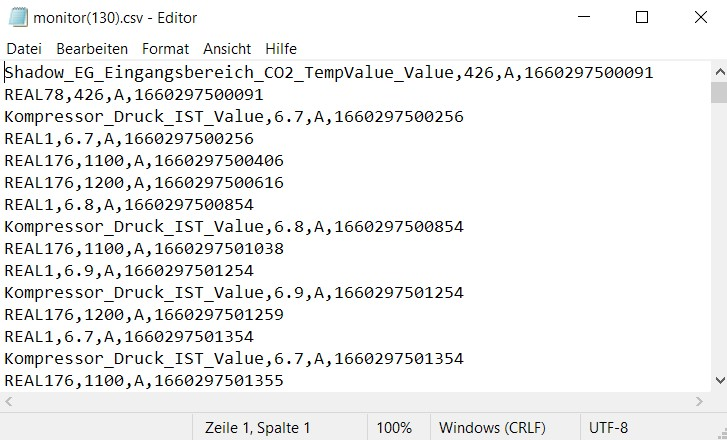
\includegraphics[scale=0.5]{pics/csvFileEditor.jpg}
    \caption{Beispiel einer CSV-Datei}
    \label{fig:impl:csvDateiEditor}
  \end{figure}
  

\begin{spacing}{1}
    \setauthor{Teresa Holzer}
    \section{HTML, CSS und Javascript [T]}\label{section:allTechHTMLCSS}
    \end{spacing}
HTML, CSS und JavaScript sind allesamt Komponenten, um eine WebSeite zu bauen. JavaScript ist dabei für die Funktionalität zuständig, CSS für das Design und HTML für den Grundaufbau.

Diese Sprachen wurden verwendet, um den zweiten Teil der Diplomarbeit, die visuelle Darstellung der Daten auf einer Website, zu realisieren.

\subsection{HTML}
% < Durchstarten mit HTML5 Autor: von: Mark Pilgrim, 2011 S. 18-23
HTML gilt als Grundgerüst einer Website. HTML besitzt sogenannte Tags, welche je über einen eigenen Nutzen verfügen. Durch diese Tags kann der Titel einer Website festgelegt werden, verschiedenste Bilder, Texte und anderer Content hinzugefügt werden. Außerdem bietet HTML die Möglichkeit, einer Webseite die passende Struktur zu verleihen. \cite{durchstartenHTML}

Um das Strukturieren einer Website zu vereinfachen, gibt es fest zugewiesene Tags. Um die wichtigsten kurz aufzulisten:
 
\begin{compactitem}
    \item [<title></title>]
    \item Definiert den Titel eines HTML Dokuments
    \item [<div></div>, <nav></nav>]
    \item Kennzeichnen eines Abschnitts bzw. einer Navigationsleiste in einem HTML Dokument
    \item [<p></p> <h1></h1>]
    \item Verantwortlich, dem HTML Dokument Text (p) und Überschriften (h) hinzuzufügen
    \item [<img> <video> <audio>]
    \item Mithilfe dieser Tags kann ein Bild/Video/Audio eingefügt werden
\end{compactitem}\cite{durchstartenHTML}

Ein Beispiel für ein HTML-File kann im nächsten Abschnitt gefunden werden, siehe Abb. \ref{lst:impl:htmlJavaScript}.
 
\subsection{CSS}
Mithilfe von CSS können Farben, Formen, Abstände und andere Designmittel einer Webseite geändert werden. CSS geht Hand in Hand mit HTML und kann jede Klasse oder auch jeden Tag, der in einem HTML-File vorkommt, ansprechen. Ein paar der wichtigsten Attribute, welche man mit CSS ansprechen und folglich verändern kann, sind: color (Farbe), width und height (Breite und Höhe eines Elements), sowie margin und padding (Abstand eines Elements zu anderen Elementen).
 
CSS kann wie JavaScript entweder direkt im HTML eingebettet \ref{lst:impl:cssEinbettung}, oder als externes File angegeben werden. Dies dient wiederum der Übersichtlichkeit und sollte je nach Größe des Projekts entschieden werden.
\cite{durchstartenHTML}

\begin{lstlisting}[language=java,caption=CSS Einbettung,label=lst:impl:cssEinbettung]
    <link rel="stylesheet" href="style.css" type="type/css" />
\end{lstlisting}
 
\subsection{JavaScript}
% < https://www.typescriptlang.org/docs/handbook/typescript-from-scratch.html
% < JavaScript für Java-Entwickler Autor: Oliver Zeigermann 2015 S9-12
JavaScript wurde ursprünglich dafür entwickelt, um als einfache Skriptsprache für kurze Code-Snippets im Browser eingesetzt zu werden. Nach einiger Zeit wurde es allerdings populärer und wurde immer öfters und für längere Codestellen eingesetzt. Webbrowser reagierten darauf positiv und optimierten die Ausführung von JavaScript. Nach dem Erfolg, den JavaScript bei Browsern feierte, wurde es unter anderem auch für node.js und JS-Server verwendet.
\cite{typeJavaScript}
JavaScript kann verwendet werden, indem es in ein HTML-Dokument eingebettet wird \ref{lst:impl:htmlJavaScript}, allerdings ist es ab einer bestimmten Größe des Programms empfehlenswert, HTML und JavaScript in verschiedene Files zu verlagern, um die Lesbarkeit zu unterstützen.
\cite{JavaScriptJavaEntwickler} 

\begin{lstlisting}[language=java,caption=HTML mit eingebettetem JavaScript,label=lst:impl:htmlJavaScript]
    <!DOCTYPE html>
    <html>
        <head>
            <title>Hello World!</title>
        </head>
        <script>
            alert('Hello World!'); // wenn die Seite aufgerufen wird, wird mithilfe von JavaScript ein Alert-Fenster mit 'Hello World!' ausgegeben
        </script>
        <body>
        </body>
    </html>
\end{lstlisting}
 
\begin{spacing}{1}
    \setauthor{Teresa Holzer}
    \section{TypeScript [T]}\label{section:allTechTypescript}
    \end{spacing}
% < https://www.typescriptlang.org/
% < JavaScript für Java-Entwickler Autor: Oliver Zeigermann 2015 S117-132
TypeScript ist eine Weiterentwicklung von Javascript, welche einige Vorteile mit sich bringt. TypeScript fügt zum Beispiel zusätzliche Syntax zu JavaScript hinzu, um eine engere Integration mit dem Editor der Wahl zu ermöglichen. Somit können Errors früher erkannt werden. TypeScript Code wird zu JavaScript Code umgewandelt und als dieser ausgeführt. Somit läuft es überall, wo auch JavaScript läuft: Dies beinhaltet einen beliebigen Browser, Node.js oder in einer App. Zusätzlich kann JavaScript auch in TypeScript verwendet werden. Ein weiterer großer Vorteil von TypeScript ist, dass es eine automatische Typendeklaration besitzt. Das heißt, dass bei der Erstellung einer Variable kein Typ mitangegeben werden muss, sondern dieser beim Kompilieren des Programms (aufgrund des Inhalts der Variable) selbst zugewiesen wird. \ref{lst:impl:automatischeZuweisung}

\cite{JavaScriptJavaEntwickler} 
\cite{TypeScriptOverview} 

\begin{lstlisting}[language=java,caption=TypeScript automatische Zuweisung,label=lst:impl:automatischeZuweisung]
    // Der Type String wird hier bei der Kompilation automatisch zugewiesen
    let helloWorld = "Hello World";
\end{lstlisting}
 
\begin{spacing}{1}
    \setauthor{Teresa Holzer}
    \section{Datenbanken [T]}\label{section:database}
    \end{spacing}

% < 1 Java ist auch eine Insel - Einführung, Ausbildung, Praxis ; von: Christian Ullenboom
Eine Datenbank ist gemeingültig dafür zuständig, viele Daten übersichtlich abzuspeichern, um diese später weiterzuverwenden. Daten gewinnen an Wichtigkeit in unserer Gesellschaft und diese verlässlich und zugänglich abspeichern zu können ist nicht mehr wegzudenken.
 
Der Grundaufbau einer relationalen Datenbank besteht aus Zeilen und Spalten, welche zusammen eine Sammlung an Daten halten. Dabei erfüllen die Zeilen die Rolle der einzelnen Elemente und die Spalten teilen die Elemente in seine Unterelemente ein. \cite{javaInselBuch}
 
 Verschiedene Arten von Datenbanken werden in den folgenden Unterkapiteln behandelt.

\subsection{H2}
% < 1 http://www.h2database.com/html/performance.html
% TODO Huemer fragen ob noch mehr zu H2 und Co
\begin{compactitem} 
    \item[Hauptmerkmale]
    \item Sehr schnell, open source, JDBC API
    \item Embedded und Server Modus, in-memory databases        
    \item Konsolen Anwendung für den Browser
    \item Das Jar-File hat nur eine Größe von 2.5 MB
\end{compactitem} 
\cite{databaseComparison}


\subsubsection{Performance (Version 2.0.202)}
Die Datenbank ist langsamer bei größeren ResultSets, da sie ab einer bestimmten Anzahl von zurückgegebenen Records zwischengespeichert werden. \cite{databaseComparison}


 
\subsection{SQLite}
% < 1 https://www.sqlite.org/index.html
% < 1 http://www.h2database.com/html/performance.html

\begin{compactitem}
    \item [Hauptmerkmale]
    \item Klein
    \item Schnell        
    \item Sehr verlässlich
    \item Stand-allone
    \item Full-featured SQL-Implementierung
\end{compactitem} 
\cite{sqlliteOfficialSite}

\subsubsection{Performance (SQLite 3.36.0.3)}
Performt etwa 2-5x schlechter bei einfachen Arbeiten auf der Datenbank. Dies führt zu einem niedrigen Arbeit-pro-Transaktion Ratio. Allerdings kann SQLite, wenn die Datenbankzugriffe komplexer werden, eine bessere Leistung erbringen. Ein wichtiger Zusatz ist allerdings, dass die Ergebnisse je nach Maschine sehr variieren. \cite{databaseComparison}

SQLite ist die meistgenutzte Datenbank der Welt und benötigt keine Administration. Die Datenbank eignet sich dadurch sehr gut für Mobiltelefone, Kameras, TV-Geräte etc., da diese ohne fachlichen Support funktionieren müssen. Auch für Websites, auf denen wenig bis mittelviele Datenbankzugriffe stattfinden, ist die SQLite Datenbank eine gute Wahl. Bei einer sehr großen Anzahl an Datenbankzugriffen, ist allerdings von einer SQLite Datenbank eher abzuraten. \cite{databaseComparison}

\subsection{PostgreSQL}
% < 1 https://www.postgresql.org/about/
% < 1 http://www.h2database.com/html/performance.html
 
\begin{compactitem}
    \item[Hauptmerkmale]
    \item Open source
    \item Objektrelationale Datenbank        
    \item Sehr mächtig
    \item Verlässlich
    \item Datenintegrität
    \item Viele Features/Add-Ons
\end{compactitem}
\cite{PostgreSQLOfficialSite}

\subsubsection{Performance (Version 13.4)}
Die Schnelligkeit der Datenbank liegt ziemlich mittig zwischen der Derby- und der H2-Datenbank, wobei sie teilweise etwas schneller als H2 abschneiden kann. \cite{databaseComparison}

 
\subsection{Apache Derby}
% < 1 http://www.h2database.com/html/performance.html
% < 1 https://db.apache.org/derby/#What+is+Apache+Derby%3F

\begin{compactitem}
    \item [Hauptmerkmale]
    \item Open source
    \item Nur 3.5 MB Größe für die Basis Engine sowie den JDBC-Driver        
    \item Basiert auf JAVA, JDBS sowie SQL Standards
    \item Derby stellt einen embedded JDBS Driver zur Verfügung, mithilfe dessen die Derby Datenbank in jede JAVA-Applikation eingebunden werden kann
    \item Supportet den Client/Server Modus
    \item Einfach zu installieren, einzurichten, sowie zu benutzen
\end{compactitem}
\cite{ApacheDerbyOfficialSite}
 

\subsubsection{Performance (Version 10.14.2.0)}
Von all den angeführten Datenbanken die Langsamste. Die Operationen auf der Datenbank werden dabei sehr schleppend ausgeführt. Ein besseres Ergebnis für Derby kann allerdings erzielt werden, wenn Autocommit ausgeschaltet wird. Die Performance wird dabei um 20\texttt{\%} besser. Um einen besseren Vergleich der Schnelligkeit heranzuziehen: Die Datenbank ist nicht einmal halb so schnell wie das erste Beispiel dieser Auflistung, die H2 Datenbank. \cite{databaseComparison}

\subsection{Wahl der Datenbank für das Projekt}
Aufgrund der großen Datenmenge, welche in dem Programm verarbeitet werden müssen, fiel die Entscheidung im Rahmen von Flexlogger auf eine PostgreSQL-Datenbank. Die Entscheidung basiert darauf, dass PostgreSQL sehr verlässlich ist und als Datenbank dafür ausgelegt ist, viele Daten speichern zu können.

\begin{spacing}{1}
    \setauthor{Teresa Holzer}
    \section{Visuelle Darstellung [T]}\label{section:gui}
    \end{spacing}
Um davor aufbereitete Daten sinnvoll visuell darzustellen, ist es wichtig, die richtigen Plattformen beziehungsweise Frameworks zu verwenden. In folgendem Kapitel werden verwendete Plattformen und Frameworks, wie Angular, BootsTrap und CanvasJS erklärt. 
% Huemer fragen 3 Zeilen zu kurz?
\subsection{Angular}
% < 1 https://angular.io/
 
Angular ist eine Plattform, um Web-Applikationen zu erstellen, welche für die Desktop- sowie für die mobile Anwendung gleichfalls funktionieren sollen. Gebaut wurde Angular in der Programmiersprache TypeScript und es inkludiert folgende Fähigkeiten:
 
\begin{compactitem}
    \item Ein Komponenten-basiertes Framework, um eine skalierbare Web-Applikation zu erstellen.
    \item Eine Sammlung von Bibliotheken, welche eine große Varietät von Features beinhaltet, Beispiele dafür sind Routing, das Management von Formularen sowie eine Client-Server-Kommunikation. Diese Bibliotheken sind laut Angular gut in die Plattform eingebunden.
    \item Eine Auswahl von Entwickler-Tools, welche hilfreich sind, um den Code zu entwickeln, zu testen, zu bauen und upzudaten.
\end{compactitem}
 
\subsubsection{Komponenten}
Komponenten sind die Baublöcke, um eine Applikation zusammenzustellen. In einer Komponente sind folgende Segmente:
 
\begin{compactitem}
    \item Ein HTML-Template
    \item Ein CSS-Style Template
    \item Einem @Component-Part, in welchem folgende Informationen geklärt werden:
    \subitem • Ein CSS-Selektor, welcher definiert, wie die Komponente in einem Template verwendet wird. Dieser Selektor kann anschließend in ein HTML-File eingebunden werden. Passiert dies, wird dieser Selektor eine Instanz der Komponente des HTML-Files.
    \subitem • Ein HTML-Template, welches Angular anleitet, wie es diese Komponente zu rendern hat.
    \subitem • Ein optionales Set von CSS-Styles, welche das Aussehen des HTML-Elements definieren.
\end{compactitem}
\cite{angularOfficialSite}
 
\begin{lstlisting}[language=java,caption=Beispiel für eine minimierte Angular Komponente,label=lst:impl:angularBsp]
    import { Component } from '@angular/core';
 
    @Component({
      selector: 'hello-world',
      template: `
        <h2>Hello World</h2>
        <p>This is my first component!</p>
      `
    })
    export class HelloWorldComponent {

    }
\end{lstlisting}
\cite{angularOfficialSite}
 
\subsubsection{Anbindung einer Angular-Applikation an einen Webserver}
% < Angular - Das umfassende Handbuch von: Christoph Höller
Um eine Anbindung an einen Webserver zu ermöglichen, stellt Angular ein Modul, welches den Namen HttpClientModule trägt, zur Verfügung. Nachdem dieses in die Klasse AppModule importiert wurde, kann es verwendet werden.
 
Wenn nun zum Beispiel die Daten eines GET-Requests aus dem Backend ausgelesen werden sollen, muss zuerst der HttpClient aufgerufen und definiert werden, ob ein GET, POST oder ein anderer Request benutzt werden soll. Diesem muss anschließend eine passende URL übergeben werden. \ref{lst:impl:angularHTTPBsp}
 
\begin{lstlisting}[language=java,caption=Beispiel für einen GET-Request,label=lst:impl:angularHTTPBsp]
  this.http.get<Animal[]>(`http://localhost:8080/api/animals`)
    .subscribe(animals => {
      this.animalArray = animals;
    });
\end{lstlisting}
 
Mit den spitzen Klammern wird dabei der Typ der übergebenen Daten definiert, in diesem Fall wäre es eine Liste des Typs Animal. Die erhaltenen Daten werden dann auf die Variable this.animalArray gesetzt. \cite{angularHandbuchBuch}
 
\subsubsection{Angular Forms}
% <  Angular - Das umfassende Handbuch von: Christoph Höller
Um in einem Angular-Projekt ein Formular verwenden zu können, muss zuerst die Forms-API hinzugefügt werden. Dies kann mit dem Befehl \texttt{npm install @angular/forms --save} umgesetzt werden. Nachdem die Module in der gewünschten Komponente eingebaut wurden, kann ein reaktives Formular (reactiveForm) erstellt werden.
 
Um auf die Eingabewerte eines Formulars zugreifen zu können, kann eine FormGroup verwendet werden. Bei dieser muss lediglich ein FormGroup-Element angelegt werden, welches die Namen der Eingabefelder trägt. \ref{lst:impl:angularFormGroup} Der linke Parameter ist dabei dazu da, einen Default-Wert festzulegen, der rechte dient dazu, eine Überprüfung der Eingabewerte zu aktivieren.
 
\begin{lstlisting}[language=java,caption=Beispiel für FormGroup eines Angular Formulars,label=lst:impl:angularFormGroup]
  this.animalForm = this.fb.group({
    animalName: [null, [Validators.required]],
    animalAge: [0, [Validators.required]],
  });
\end{lstlisting}
 
Das zugehörige HTML-Form hat in der Praxis diese Form:  \ref{lst:impl:angularFormHTML}
 
 
\begin{lstlisting}[language=java,caption=Beispiel für ein reaktives Formular,label=lst:impl:angularFormHTML]
  <form [formGroup]="animalForm">
        <label>Tier Name</label>
        <input formControlName="animalName" type="text">
        <label>Tier Alter</label>
        <input formControlName="animalAge" type="number">
      </form>
\end{lstlisting}
\cite{angularHandbuchBuch}
 
 
\subsection{Bootstrap}
% https://getbootstrap.com/
Mithilfe von Bootstrap können schnelle und responsive Seiten gebaut werden. Bootstrap ist leistungsstark, erweiterbar und mit vielen Features versehen. Bootstrap stellt vielzählige Variablen für Farben, Schriftstile und mehr auf :root-Ebene zur Verfügung, welche überall verwendet werden können. Bei Komponenten sind CSS-Variablen auf die jeweilige Klasse beschränkt, können aber leicht geändert werden. Bootstrap kann im Allgemeinen großflächig individuell angepasst werden.
\cite{bootstrap}

Bootstrap wurde gemeinsam mit CSS verwendet, um das Aussehen der Flexlogger-Website anzupassen.


\subsection{CanvasJS}
\label{subsection:canvasJS}
% < 1 https://canvasjs.com/
 
CanvasJS ist ein Framework, mit welchem sich Diagramme erstellen lassen. Es besitzt eine Integration in Angular. Auf der CanvaJS Website auf der Unterseite für Angular können unterschiedlichste Diagramme mit dem passenden Komponenten-, Modul- sowie HTML-Code gefunden werden.
\cite{canvasJsOfficialSite}

Um CanvasChart in Angular zu verwenden, müssen verschiedene Codeteile eingefügt werden. Diese beinhalten einen HTML-Teil, welcher das Chart anzeigt. \ref{lst:impl:canvasJSHTML}
 
\begin{lstlisting}[language=html,caption=CanvasJS HTML,label=lst:impl:canvasJSHTML]
  <canvasjs-chart [options]="chartOptions" [styles]="{width: '100%', height: '360px'}"></canvasjs-chart>
\end{lstlisting}
 
Anschließend müssen Dateien, welche auf der canvasJS-Seite heruntergeladen werden können, in die Dateiordner des gewünschten Angular-Projekts kopiert werden. Diese tragen die Namen \texttt{canvasjs.min.js} und \texttt{canvasjs.angular.component.ts}.
 
Der vorletzte Schritt beinhaltet das Importieren des CanvasJSChart-Moduls.
Im letzten Schritt werden im TypeScript-File der Komponente, in der das Diagramm angezeigt werden soll, die Diagrammoptionen für das Diagramm festgelegt. Diese beinhalten in der einfachsten Form den Titel und die Daten, kann aber erweitert werden. \ref{lst:impl:canvasJSchartOptions}
 
\begin{lstlisting}[language=html,caption=CanvasJS chartOptiones,label=lst:impl:canvasJSchartOptions]
  chartOptions = {
    title: {
      text: "Basic Column Chart in Angular"
    },
    data: [{
      type: "line",
      dataPoints: [
        { label: "Apple",  y: 10  },
        { label: "Orange", y: 15  }
      ]}]};
\end{lstlisting}
 
\cite{canvasJsOfficialSite}

\begin{spacing}{1}
    \setauthor{Teresa Holzer}
    \section{Quarkus [T]}\label{section:quarkus}
    \end{spacing}
% < 1 https://quarkus.io
% < 1 https://books.google.at/books?hl=de&lr=&id=AH_EDwAAQBAJ&oi=fnd&pg=PP1&dq=quarkus&ots=ZJfLHasMm9&sig=K7__BsdmoksvoLfJSrqqGOPac1Y&redir_esc=y#v=onepage&q=quarkus&f=false
 
Quarkus wurde kreiert, um Applikationen zu erstellen, welche in einer modernen, cloud-nativen Welt funktionieren sollen. Quarkus ist ein kubernetes-natives Java-Framework, auf GraalVM und HotSpot zugeschnitten. Das Ziel von Quarkus ist es, Java zur führenden Plattform für Kubernetes und serverlose Umgebungen zu machen und Mikroservicearchitekturen-Komponenten zusammenzufügen. Quarkus ist open-source. \cite{quarkusOfficialSite}
 
Die größte Challenge von Mikroservicearchitekturen ist, dass die Vermehrung von Services die Komplexität des Systems erhöht. Diese kann mithilfe von Kubernetes-basierenden orchestrierenden Systemen gelöst werden, da somit die Effizienz sowie die Ressourcenverwertung erweitert werden können. Die Systeme regeln die zeitliche Planung und das Management der Mikroservices in einer dynamischen Weise. Dadurch kann man auch je nach Bedarf an dem System arbeiten, ohne dass die Gefahr besteht, dass ein Container ausfällt. Um nun die gesamten Komponenten zusammenzufügen, wurde das Framework Quarkus entwickelt.
 
Quarkus wird vor allem dann verwendet, wenn es darum geht, cloud-native Applikationen von Unternehmen zu managen. Es ist in der Lage, kurzen nativen Code aus Java Klassen zu bauen, sowie Container-Images daraus zu erstellen. Diese Container können darauffolgend auf Kubernetes laufen. Außerdem unterstützt Quarkus die bekanntesten Java Libraries wie etwa RESTEasy, Hibernate, Apache Kafka, Vert.x, usw.
 
Wie bereits erwähnt, ist eines der Features von Quarkus die Fähigkeit aus Applikationen automatisch Container-Images zu generieren. Durch das Generieren von Container-Images aus nativen Applikationen wird außerdem eine Gefahr zunichte gemacht: Konfliktfehler von Errors, wenn der Build auf einem anderen Operating System stattfand und das Programm nativ ausgeführt wird.
Quarkus sorgt außerdem dafür, imperative und reaktive Modelle zu verbinden. Reaktives Programmieren wird immer beliebter aus dem Grund, dass es in der Lage ist, asynchrones programmieren mit Daten-Streams und der Veränderung von Daten zu verbinden. \cite{QuarkusBuch}
 
\subsection{Architektur}
Im Zentrum von Quarkus liegt die Kern-Komponente, welche die Aufgabe hat, die Applikation in der Build-Phase umzuschreiben, um sie zu optimieren \ref{fig:impl:QuarkusArchitektur}. Daraus entsteht eine native ausführbare und Java-runnable Applikation. Damit der Quarkus-Kern diese Arbeit erledigen kann, müssen einige verschiedene Komponenten zusammenarbeiten:
 
\begin{compactitem}
    \item Jandex: Ein platzsparender Java-Annotation-Indexer, sowie eine offline Reflexions-Library. Diese Bibliothek ist in der Lage, alle runtime-sichtbaren Java Annotationen und Klassenhierarchien für ein Set von Klassen in einer speichereffizienten Repräsentation zu indexen.    
    \item Gizmo: Gizmo ist eine Bytecode-Generations-Library, welche von Quarkus verwendet wird, um Java Bytecode zu produzieren.             
    \item GraalVM: Ein Set von Komponenten, in welchem jede eine bestimmte Funktion hat. Beispiele dafür sind: ein Compiler, ein SDK API für die Integration von Graal Sprachen und der Konfiguration von native images, runtime Umgebung für JVM-basierte Sprachen
    \item SubstrateVM: SubstrateVM ist eine Unterkomponente von GraalVM, welche die ahead-of-time (AOT) Kompilation von Java Applikationen von Java Programmen zu eigenständigen ausführbaren Programmen erlaubt.
\end{compactitem}
 
Des Weiteren gibt es noch einige Quarkus Extensions. Dazu gehören die MicroProfile Spezifikationen, sowie ein Set von Extensions für Hibernate ORM, ein Transaktionsmanager (Narayana), ein Verbindungs-Pool-Manager und viele mehr. \cite{QuarkusBuch}
 
\begin{figure}
    \centering
    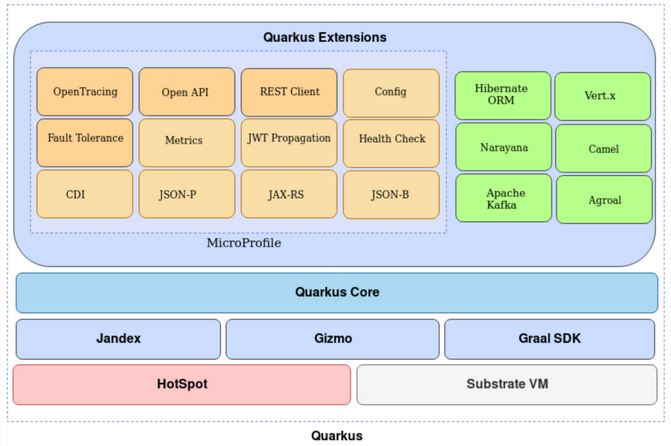
\includegraphics[scale=0.9]{pics/quarkusArchitektur.JPG}
    \caption{Quarkus Architektur \cite{QuarkusBuch}}
    \label{fig:impl:QuarkusArchitektur}
\end{figure}
 
% \subsection{Funktionen}
\subsection{Vergleich zu anderen Tools}
% < https://devm.io/java/micronaut-speed-test-170870-001
% < https://micronaut.io/2020/04/07/micronaut-vs-quarkus-vs-spring-boot-performance-on-jdk-14/
Drei sehr vergleichbare Frameworks sind Quarkus, Micronout und Spring Boot. Sie besitzen alle ähnliche Features und Fähigkeiten.
Am wichtigsten ist dabei, welches Framework  am schnellsten ist, welches am performantesten und welches  den wenigsten Speicher benötigt.
\cite{Micr/QuarBenchmark}
 
\begin{compactitem}
    \item[Quarkus]
    \item Kubernetes-native, für Java designed, für GraalVM und OpenJDK Hotspot, besitzt die besten Java-Bibliotheken und Standards, schnell beim Starten
    \item[Micronout]
    \item Cloud-native, JVM-basiert, full-stack Framework für Mikro-Services und serverlose Anwendungen, geringer Speicherverbrauch
    \item[Spring Boot]
    \item Open-Source Java Framework, einfach um stand-alone Anwendungen und Mikroservices zu kreieren, benötigt sehr wenig Konfiguration, um starten zu können
\end{compactitem}
\cite{Micr/QuarBenchmark}
 
Für einen näheren Vergleich zwischen den Frameworks, siehe \ref{fig:impl:Quarkusbenchmark}. Dabei kann erkannt werden, dass Quarkus Response Zeit die bestbewertete ist, Spring trotzt dabei mit einer Compilation Zeit von nur 1.33s, wenn der Befehl \texttt{./mnv clean compile} verwendet wird. Insgesamt kann allerdings aus dem Benchmark Vergleich gezogen werden, dass Micronout in den meisten Kategorien als Sieger hervorgeht. Vor allem, wenn ein kleiner Speicherverbrauch wichtig ist, sollte zu Micronout gegriffen werden. \cite{MicrVSQuarVSSprin}
 
\begin{figure}
    \centering
    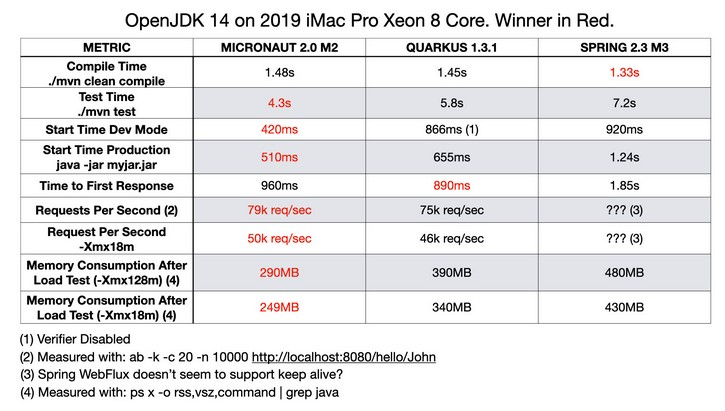
\includegraphics[scale=0.8]{pics/quarkus_benchmark.jpg}
    \caption{Quarkus Benchmark Test \cite{MicrVSQuarVSSprin}}
    \label{fig:impl:Quarkusbenchmark}
\end{figure}
 
%\subsection{NodeJS im Vergleich}

\subsection{http GET/POST/PUT Funktionen}
% < 1 https://quarkus.io/guides/rest-json
Mithilfe von GET/POST/PUT können Daten von einem Webserver geholt, oder an diesen geschickt werden, um diese später z.B. in einer Webapplikation nutzen zu können.
%Was macht jeweils GET POST PUT?
 
Um diese Annotations verwenden zu können, muss eine REST Ressource erstellt werden.
Bei dieser Ressource muss als erstes ein Pfad definiert werden. Dieser gilt für alle darauffolgenden Funktionen in der Ressource Klasse.
 
Die Funktionen in der Klasse sind alle für verschiedene GET- bzw. POST-Requests mit verschiedenen Pfaden verantwortlich. Bei jedem von ihnen wird definiert, ob ein GET, POST oder PUT Request abgesetzt werden soll. In der darauffolgenden Zeile wird ein Pfad angegeben, welcher zusätzlich nach dem über der Klasse angegebenen Pfad verwendet wird. Als letztes Attribut wird definiert, je nachdem ob der Request etwas auslesen soll oder etwas anzeigen lassen soll, ein @Produces bzw. ein @Consumes. In diesen wird jeweils der Typ von dem auszulesenden bzw. anzuzeigenden angeführt. In dem Beispiel unterhalb ist es ein JSON-Format. \cite{quarkusRest}
\begin{lstlisting}[language=java,caption=Quarkus POST-Request,label=lst:impl:canvasJSchartOptions]
    @GET
    @Produces(MediaType.APPLICATION_JSON)
    @Path("/all/animal")
    public Set<Animal> getAll() {
        return animalRepository.getAll();
    }
  \end{lstlisting}


 
\subsection{JPA und JDBC}
% < 1 https://quarkus.io/guides/hibernate-orm
% < Java ist auch eine Insel, Christian Ullenboom, 2018 S1111-1121 

%  < https://books.google.at/books?hl=de&lr=&id=UHobxmgB714C&oi=fnd&pg=PR1&dq=jpa&ots=ijY_GdSJ5U&sig=IlRJxhMjrF4xF2-NXQ-OdM6f48Q&redir_esc=y#v=onepage&q=jpa&f=false, von  Mike Keith S5-16


\begin{compactitem}
    \item [JPA]
    \item JPA ist die Abkürzung für Jakarta Persistance API. Es ist ein POJO-basiertes Framework für Java Persistance. Die Hauptaufgabe von JPA ist dabei das objekt-relationale Mapping, allerdings bietet JPA auch Lösungen für die architektonische Herausforderung der Integrierung von Persistance an.
    \item [JDBC]
    \item Um in Java auf eine relationale Tabelle Zugriff zu erhalten, wird JDBC benötigt. JDBC ist dabei eine Abkürzung für Java Database Connectivity. JDBC fasst einen Satz von Schnittstellen zusammen, welcher nötig ist, damit sich Java an relationale Datenbanken anbinden kann. Durch JDBC kann somit eine Verbindung zu einer Datenbank aufgebaut, auf Tabellen zugegriffen und Daten ausgelesen oder verändert werden.  
\end{compactitem}
\cite{quarkusHibernate}

\subsection{Quarkus und JDBC}
Um Quarkus in Verbindung mit Datenbanken verwenden zu können, muss ein passender JDBC-Driver verwendet werden. Dabei gibt es für jede Datenbank einen eigenen passenden Driver. Bei einer PostgreSQL-Datenbank, welche in diesem Projekt verwendet wurde, lautet die artifactID (welche verwendet wird, um den JDBC-Driver als Dependency einzubinden), \texttt{quarkus-jdbc-postgresql}. \ref{lst:impl:JDBCDependency} Diese Dependency muss in die pom.xml Datei des Programms kopiert werden. Beim Starten des Projekts wird der JDBC-Driver anschließend automatisch hinzugefügt. \cite{quarkusHibernate}


\begin{lstlisting}[language=html,caption=JDBC Dependency,label=lst:impl:JDBCDependency]
    <dependency>
        <groupId>io.quarkus</groupId>
        <artifactId>quarkus-jdbc-postgresql</artifactId>
    </dependency>
  \end{lstlisting}



\begin{spacing}{1}
    \setauthor{Teresa Holzer}
    \section{SQL [T]}\label{section:sql}
    \end{spacing}
\subsection{Allgemein}

\subsection{Wie SQL funktioniert}

\subsection{Kommunikation mit Datenbanken}



\begin{spacing}{1}
    \setauthor{Pouget Marcel}
    \section{Beckhoff [M]}\label{section:allTechBeckhoff}
    \end{spacing}
 

Beckhoff ist ein internationales Unternehmen, welches 1980 von Hans Beckhoff gegründet wurde. Das Unternehmen realisiert offene Automatisierungssysteme. Bekannt wurde das Unternehmen vor allem in dem Bereich Industrie-PC und das zugehörige Softwaresystem Twincat. Die Produkte, welche von Industrie-PCs, Steuerungssystemen und Softwaretools reichen, werden vor allem in der Gebäude-Automatisierung und für die Steuerung von Maschinen verwendet. Konkret geht es um automatisierte Prozesse, die vor allem in der Fertigung eine große Rolle spielen. Auch die Effizienz und die Energiebilanz des Anwenders können gesteigert werden. In der Firma Flexsolution kann mit den Systemen von Beckhoff vom Licht, über Schalosien und Fertigungsmaschinen alles gesteuert werden.   

Entwickelt werden solche Anwendungen in der Software Twincat mit einer von Beckhoff entwickelten Programmiersprache.   

  

Twincat bietet den Vorteil, dass die Codeänderungen schnell und unkompliziert angepasst werden. So können, ohne dass etwas kompiliert werden muss, Anpassungen getätigt werden. Außerdem sieht man, während das Programm läuft, direkt die Werte der Variablen. Dies erlaubt es, schnell einzugreifen und alles zu überwachen.

\begin{figure}[h t]
    \centering
    \includegraphics[scale=0.2]{pics/twincat übersicht.png}
    \caption{So sieht die Twincat Übersicht aus}
    \label{fig:impl:TwincatÜbersicht}
  \end{figure}

  Eine weitere Besonderheit ist die Art, wie der Code ausgeführt wird. Denn in einer Beckhoff-Steuerung wird nach einem festgelegten Zyklus der Programmcode von oben nach unten ausgeführt. Es werden dabei nur Operationen wie "if, iflse“, mathematische Operationen, Zuweisungen und timer unterstützt.   

Um das Warten der Software für die Mitarbeiter der Firma einfach zu gestalten, wurde nach Abschluss des Projektes die Funktion des Chargecontrollers mit der Hilfe eines Mitarbeiters für Beckhof optimiert. Dies gibt den Mitarbeitern die Möglichkeit, die Software zu erweitern, auf mögliche Bugs zu reagieren oder Änderungen durchzuführen. Durch die Anpassung für Twincat werden dem zuständigen Mitarbeiter die Deployments auf dem Raspberry Pi erspart.   

\begin{figure}[h t]
    \centering
    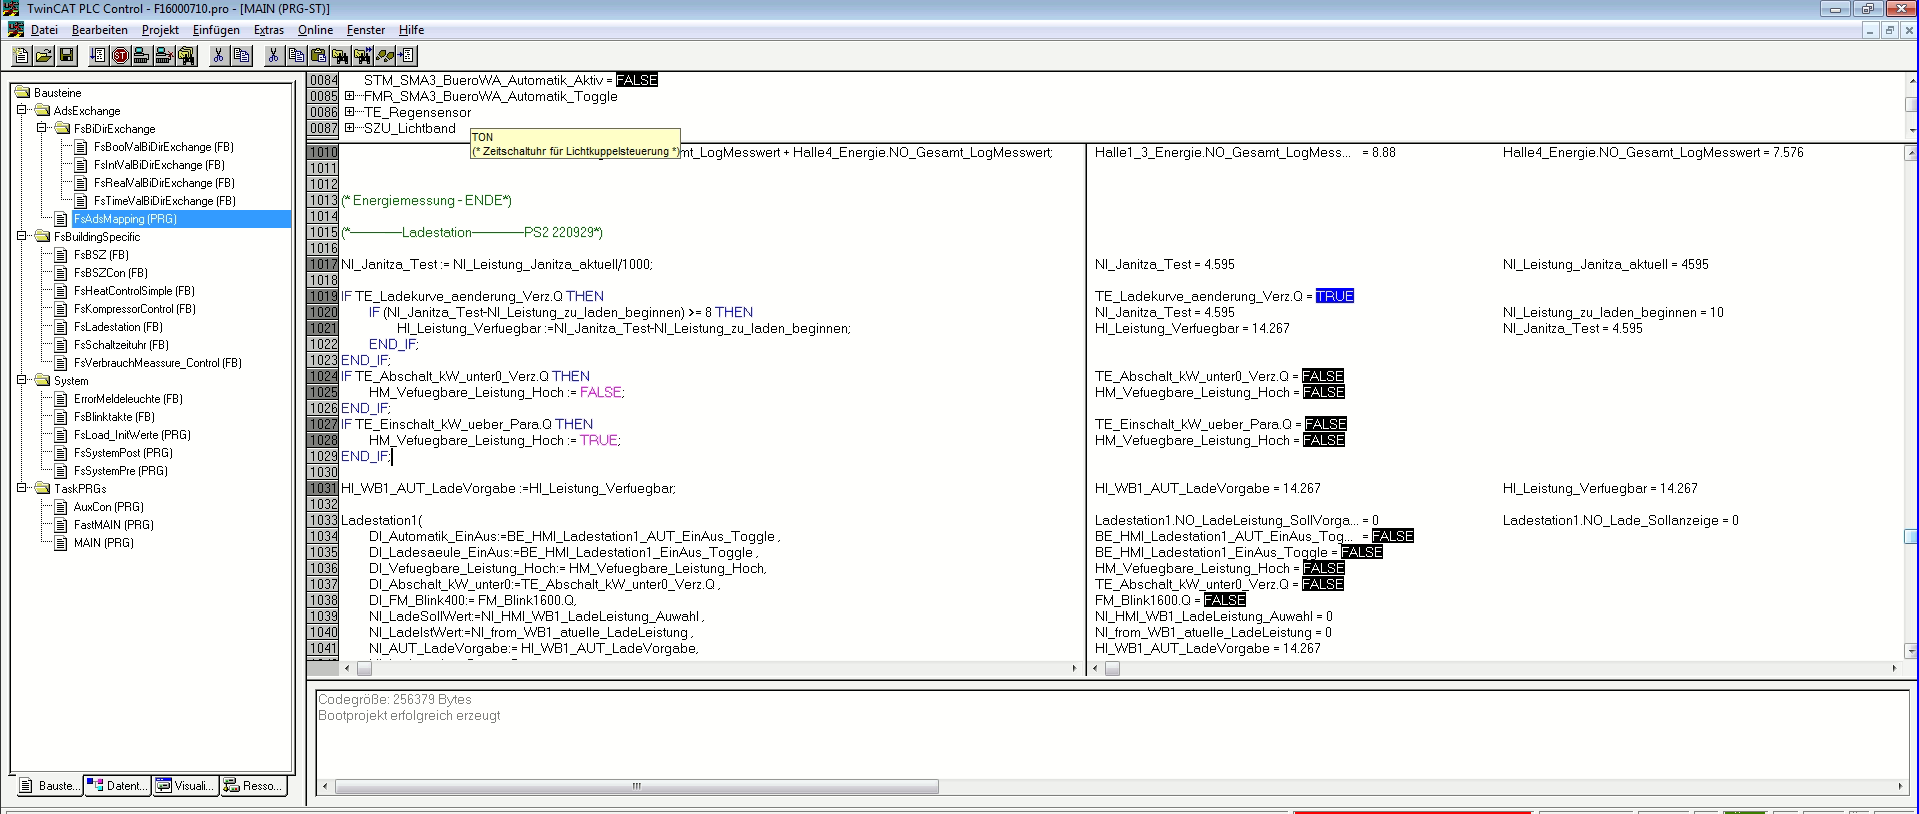
\includegraphics[scale=0.2]{pics/LadestationTwincat.png}
    \caption{Abschnitt der Wallboxen in Twincat}
    \label{fig:impl:TwincatWallbox}
  \end{figure}
 
\begin{spacing}{1}
    \section{Raspberry [M]}\label{section:allTechRaspberry}
    \end{spacing}
Ein Raspberry Pi, oft auch nur 'PI' genannt, ist ein vollwertiger Einplatinen-Computer. Das bedeutet, dass alle Komponenten, die in jedem Computer zu finden sind, auf einer einzigen Platine zu finden sind. Ausnahme dafür ist das Netzteil, welches meist aus einem 5 Volt USB C Kabel besteht. Als Betriebssystem wird das Linux-basierte System Raspberry Pi OS angeboten. Dieses besteht aus einem Desktop, einem Webbrowser, Einstellungen und Editoren für verschiedene Programmiersprachen. Der Mini-PC unterstützt jedoch auch andere Systeme, wie Raspberry Pi OS Lite, welches fast reines Linux ist. Dort findet gibt es weder eine graphische Oberfläche noch vorinstallierte Apps.

\begin{figure}[h t]
  \centering
  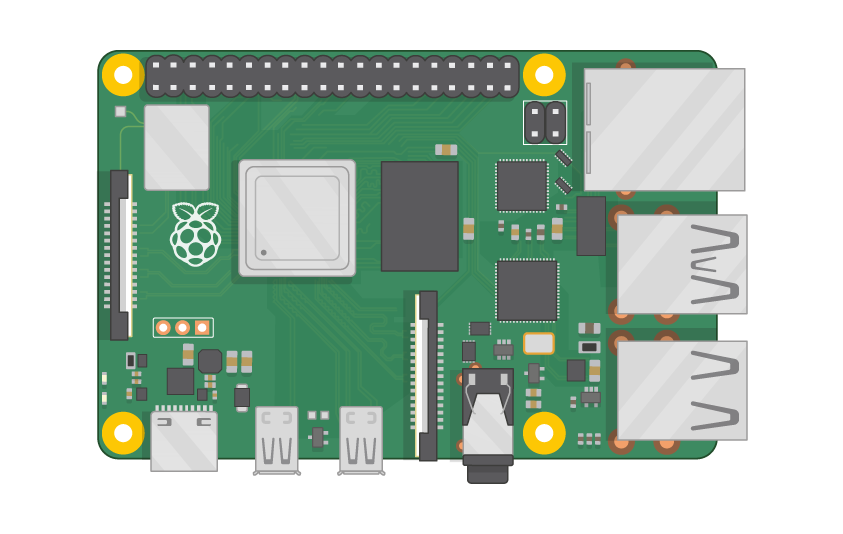
\includegraphics[scale=0.5]{pics/raspberry-pi.png}
  \caption{Aufbau eines Raspberry Pis}
  \label{fig:impl:RaspiAufbau}
  \cite{raspyimage}
\end{figure}



Da diese Mini-PCs in vielen Ausführungen und noch dazu relativ günstig zu haben sind, wurde für das Projekt ein Raspberry PI 4 ausgewählt. Dieser hat 4 GB RAM, eine Micro-SD-Karte mit einem vorkonfigurierten Image, einem Netzwerkanschluss und 4 USB-Steckplätze. Um die Zuverlässigkeit des Systems gewährleisten zu können, wurde ein Gehäuse von der Firma Flexsolution entwickelt, welches mit einem eingebauten Lüfter die Platinen kühlt. Des Weiteren wurde ein Modul installiert, welches einen Akku beinhaltet und den PI über eine 12 Volt-Leitung mit Strom versorgt. Dies ermöglicht eine Absicherung für Stromausfälle. Der Raspberry wurde in einem Schaltschrank montiert und an das Netzwerk angeschlossen.



Solche Raspberrys werden in der Firma oft verwendet, da sie sich perfekt für die Flextask eignen. Sie sind günstig, leise, klein und verbrauchen kaum Strom. Sie können mit sogenannten GPIO-Pins mit Hardware interagieren und bieten eine Vielzahl an Möglichkeiten, Module anzuschließen.

\cite{aboutRaspberry}
\cite{raspberryChip}
 



\begin{spacing}{1}
\chapter{Wallbox [M]}\label{chapter:wallbox}
\end{spacing}
Dieses Kapitel beschäftigt sich mit dem Aufbau der Wallboxen, der Struktur der Firma und den Funktionen der Applikation zur Steuerung der Ladestationen. Für das Projekt werden Librarys verwendet, welche von der Firma intern entwickelt wurden. Diese werden dazu genutzt, um Daten zwischen den Wallboxen und dem Webinterface auszutauschen. Untersucht wird in diesem Teil der Arbeit, wie die Daten über die verschiedenen Netzwerkschichten transportiert werden können. 


\begin{spacing}{1}
    \section{Untersuchungsanliegen}\label{section:untersuchungsanliegen}
    \end{spacing}
Das ist ein Test, um zu schaun, ob es so funktioniert, wie ich mir das vorstelle

\begin{spacing}{1}
    \section{Ist-Stand}\label{section:ist-standWallbox}
    \end{spacing}
Zu der Zeit vor dem Projekt ist es der Firma nicht möglich, 
Elektro-Fahrzeuge aufzuladen. Um das erreichen zu können, 
soll auf dem Dach des Firmengeländes eine Photovoltaik Anlage 
installiert werden, welche mit bis zu 170 kWh die Firma und die 
neuen E-Autos mit Strom versorgen kann. Die eigens dafür angeschafften 
Elektroautos sollen mit 5 Wallboxen der Marke "I-CHARGE CION" beladen 
werden. Da es bis zu dem Zeitpunkt des Startes des Projekts keine 
Möglichkeit gab, jene Wallboxen anzusteuern und überwachen zu können, 
beschäftigt sich dieser Teil der Diplomarbeit mit diesen Themen. 


\begin{spacing}{1}
    \section{Aufbau des Projektes}\label{section:aufbaudesProjektesWallbox}
    \end{spacing}
\subsection{Beschreibung der Funktionen}
%% sehr einfache Beschreibung der Website mit vielen Screenshots von de einzelnen Komponenten (Button/ EinagbeFeld / was wird wann angezeigt etc.)


\subsection{Logger}
Das sogenannte FS-Logger-Programm setzt sich aus mehreren Klassen zusammen, wie etwa einen DataJDBCAdapter, einer Hauptklasse namens FlexTaskFsLogger. Weiteres befindet sich in dem Programm eine Modelklasse namens LogEntry, welche die Attribute der eingetragenen LogEntries definiert. Um die einen reibungslosen Ablauf zu garantieren, wird eine Blocking-Queue verwendet, welche Multithreading unterstützt. Das ganze Programm baut auf dem Producer Consumer Pattern auf.	

\subsubsection{DataJDBCAdapter}
Der DataJDBCAdapter ist dafür verantwortlich, eine Verbindung zu der PostgreSQL-Datenbank aufzubauen und somit die benötigten Objekte in einer Datenbank abzuspeichern (insert). Um diese Verbindung herzustellen, verwendet der JDBCAdapter eine URL, welche in einem String abgespeichert ist, sowie einen Usernamen und ein Passwort. Innerhalb der connect-Methode werden diese Daten verwendet, sie gibt ein Connection Objekt zurück, welches angibt, ob die Verbindung zur Datenbank erfolgreich war. Die connect-Methode wird innerhalb der darunterliegenden insertLogEntry-Methode aufgerufen. Wenn die Anbindung erfolgreich war, wird ein PreparedStatement mithilfe des vorher übergebenen SQL-String erstellt und darauffolgend ausgeführt. Somit wird erfolgreich ein neuer Datenbankeintrag in der Datenbank gespeichert. Falls während des ganzen Ablaufes ein unerwarteter Fehler auftauchen sollte, wird dieser mittels einer Java-Exception in die Konsole geschrieben.

\subsubsection{Main Klasse FlexTaskFsLogger}
Die Klasse FlexTaskFsLogger ist die Main-Klasse des Programms. Sie führt das Programm aus. Dieser Klasse werden auch folgende Methoden vererbt, da sie eine Subklasse der Klasse FlexTask ist: 
\begin{compactitem}
    \item getNeededTaskParameters
    \item getNeededDeviceParameters
    \item isSingleDeviceTask
    \item closing
    \item initTask
\end{compactitem}

Zusätzlich befindet sich noch in der Klasse eine Getter- und Setter-Methode, diese sind allerdings lediglich für eine Zählvariable zuständig, um bestimmte Daten weniger oft in die Datenbank einzuspeichern.

Das Haupmethode des FlexTaskFsLogger ist die initTask-Methode. In ihr wird eine BlockingQueue mit dem generic Type LogEntry erstellt. Mithilfe dieser Blocking-Queue wird darauffolgend ein Producer und ein Consumer erstellt, welche die Blocking-Queue als Parameter übergeben bekommen. Nachfolgend werden jeweils zwei Producer-Threads und zwei Consumer-Threads erstellt und gestartet. Um eine zeitliche Einteilung zu haben, wird ein sogenannter TimerTask erstellt, welcher wiederum auch ein neuer, unabhängiger Thread ist. Er wird dazu genutzt, um in einem gewissen Intervall Methoden oder Code-Blöcke aufzurufen. In diesem Fall wird der Task dazu verwendet, über den DataJDBCAdapter einen neuen Eintrag in die Datenbank zu speichern. Dazu wird zuallererst überprüft, ob eine Variable, welche für das Starten und Stoppen des Tasks zuständig ist, auf true gesetzt wurde. Anschließend wird ein sogenannter StringBuilder, welcher aus einer Kette von Strings besteht, aus dem vorher erstellten Consumer geholt. Dieser StringBuilder besteht aus einem aneinandergeketteten Insert-Statement. Um die Ausführbarkeit des Stringbuilders zu gewährleisten, muss die letzte Stelle (an welcher sich ein Beistrich befindet) gelöscht werden und durch einen Strichpunkt ersetzt werden. 

Um das korrekt erstellte SQL-Statement nun ausführen zu können, wird in einem try and catch Statement die insertLogEntry-Methode des DataJDBCAdapter ausgeführt. Dabei wird der StringBuilder mit dem SQL-Statement, welche mithilfe der toString-Methode in einen String umgewandelt wird, übergeben. 

Anschließend wird der eben verwendetet StringBuilder geleert, indem die delete-Methode aufgerufen wird. Um einen neuen Insert-Aufruf zu ermöglichen, wird ein insert-Header (siehe Abb.1) über die setStringBuilder-Methode aus dem Consumer gesetzt. 

Nun wird der vorher beschriebene TimerTask in einem eine Zeile davor erstellten Timer als Parameter übergeben.

Der nächste Abschnitt sorgt dafür, dass man das Programm, also den Consumer und Producer aus- und einschalten kann. Dazu werden zuerst zwei Datenpunkte initialisiert. Diese werden durch das Setzen einer spezifischen Adresse und dem Namen eines Datenpunkts erstellt. Dabei ist der Datenpunkt \texttt{logger\_nav\_status\_icon\_Click} dazu verantwortlich, darauf zu hören, ob sich ein Wert, welcher in diesen Datenpunkt gespeichert ist, geändert hat. Das heißt, wenn auf der eigens dafür erstellten Website der Ein- und Ausschaltknopf gedrückt wird, wird der Timer pausiert und das Programm schreibt keine Werte mehr in die Datenbank. Im Gegensatz dazu ist der \texttt{logger\_nav\_status\_icon\_State} dafür da, einen Wert für die Website zu übergeben. Damit wird die Farbe des Icons verändert, um dem User ein Feedback zu seiner Aktion zu geben.
Nachdem die Methode setDatapointChangedCommand mit dem \texttt{logger\_nav\_status\_icon\_Click} verbunden wird, wird aktiv auf den Datenpunkt gehört. Ein neuer DatapointCommand wird dabei übergeben, in ihm wird die execute-Methode überschrieben. In dieser Methode wird zuallererst eine temporäre Variable erhöht, sie ist dafür da jeden zweiten Dateneintrag zu überspringen, da die HMI jedes Mal zwei Werte schickt, allerdings nur einer benötigt wird. In Folge darauf wird in einem If-Statement der Wert des \texttt{logger\_nav\_status\_icon\_State} Datenpunkts geändert, um die Farbe des Einschalt Icons zu verändern. Zusätzlich wird die startOrStop Variable auf false gesetzt und der Producer und der Consumer werden mithilfe der Übergabe von ‚false‘ in der setRun-Methode gestoppt. Im else-Zweig des If-Statement wird genau das gegenteilige bewirkt, d.h. Producer und Consumer werden gestartet und die \texttt{logger\_nav\_status\_icon\_State} wird wieder auf den ursprünglichen Wert geändert. 

\subsubsection{LogEntry Klasse}
Dies ist die Model-Klasse des Programms. In ihr werden die Attribute des LogEntries festgelegt. Diese beinhalten die dp-id, d.h. die Id des Datenpunktes, welcher gespeichert werden soll. Außerdem wird der Wert des Datenpunktes, die Einheit und der Timestamp, also den genauen Zeitpunkt, an welchem der LogEntry erstellt wurde, angelegt. In der Klasse befinden sich zusätzlich Getter und Setter für die Attribute und ein Konstruktor. 

\subsubsection{Blocking Queue - Producer }
Diese Klasse ist der Producer der Blocking Queue, d.h. in dieser Klasse werden die Objekte in die Blocking Queue hinzugefügt. 

Es lassen sich zwei Attribute im Producer finden, die Blocking Queue, in welche die Objekte später hinzugefügt werden und eine Boolean Variable, welche den Namen “run” trägt. Sie ist dafür verantwortlich, den Producer zu deaktivieren bzw. zu aktivieren. Unterhalb der Attribute befinden sich ein Konstruktor, um die Blocking-Queue zu übergeben und ein Getter und ein Setter für die run-Variable. 

Die Hauptmethode der Klasse ist die run-Methode. Hier wird ein neuer DatapointCommand erstellt, in welchem die execute-Methode überschrieben wird. Innerhalb der execute-Methode wird ganz oben eine Counter Variable initialisiert, sie ist dafür verantwortlich, bestimmte Daten von Datenpunkte nur jedes zweite Mal in die Blocking Queue hinzuzufügen. Danach befindet sich ein if-Statement, welches überprüft, ob der Code im Consumer ausgeführt werden soll oder nicht. In diesem if-Statement befindet sich ein Switch für den specificDataType, welcher je nach DataType einen bestimmten Codeteil ausführt. In dem einen Codeteil wird die counter-Variable auf true oder false überprüft (bei einem false wird der Datenteil nicht in die Blocking-Queue hinzugefügt), in dem anderen wird dies ignoriert.

Allerdings kümmern sich beide Codeteile darum, die jeweiligen Daten als LogEntry zu erstellen und diesen anschließend in die Blocking Queue zu pushen.

Mithilfe des Codes, welcher sich unterhalb des erstellten DataPointCommands befindet, wird über die Datenpunkte des jeweiligen Geräts iteriert und sorgt dafür, dass der oben liegende Codeteil bei einer Änderung ausgeführt wird.  

\subsubsection{Blocking Queue - Consumer }
In dieser Klasse geht es um den Consumer der Blocking Queue, d.h. vom Consumer werden Objekte aus der Blocking Queue genommen und diese weiterverarbeitet. Die Attribute in dieser Klasse sind so wie in der Producer Klasse eine Blocking-Queue, sowie die run-Variable, um den Consumer zu aktivieren bzw. zu deaktivieren. Im Konstruktor wird wiederum die Blocking-Queue übergeben.

In der run-Methode der Klasse wird in einem while-True ein if-Statement ausgeführt, in welchem sich ein try- and catch-Statement befindet. In diesem wird das benötigte Objekt aus der Blocking-Queue geholt und anschließend in einen StringBuilder als gültiges SQL-Statement hinzugefügt.

Unterhalb befindet sich noch eine Getter- und Setter-Methode für den StringBuilder sowie die run-Variable.

\subsection{Quarkus Backend (Beschreibend)}
Das Backend besteht aus JAVA und dem Java-Framework Quarkus. 

\subsubsection{LogEntry Klasse}
Hier werden die Attribute des LogEntries festgelegt. Diese beinhalten wie auch im Programm FlexTaskFsLogger die dp-id, den Wert, die Einheit und einen aktuellen timestamp des Eintrags. 
Auch beinhaltet ist ein Konstruktor, Getter- und Setter-Methoden für die Attribute sowie eine toString-Methode, um die Attribute formatiert zurückgeben zu können. 

\subsubsection{LogEntry Ressource}
Mithilfe dieser Klasse werden bestimmte Daten an bestimmte vorher definierte Adressen geschickt. 
Der vorher definierte Path ‚/logEntry‘ wird dabei bei jeder Anfrage am Anfang der Adresse verwendet. 
Um das davor erstellte LogEntry Repository zu verwenden, wird es am Anfang der Methode mit dem Schlüsselwort new initialisiert.

In der Ressource befinden sich verschiedenste GET-Methoden, welche alle einen anderen Nutzen haben: 

\begin{compactitem}
    \item getAll(): Hier wird durch die Übergabe der Parameter definiert, in welchem Zeitraum die benötigten Daten zurückgegeben werden. Diese Parameter werden mithilfe von PathParam übergeben, d.h. die Daten werden über die URL übergeben. Zusätzlich steht über der Methode ein \texttt{@Produces(MediaType.APPLICATION\_JSON)}, um festzulegen in welchem Format der Rückgabewert zurückgeben wird. In diesem Fall ist es das JSON-Format.
    \item getByName(): Diese Methode ist sehr ähnlich zur getAll()-Methode. Lediglich wird ein zusätzlicher Name übergeben und somit die getByName-Methode des Repositories verwendet. 
    \item getCSV(): In dieser Methode wird im Pfad neben den Daten ein filePath angegeben, in welchem die CSV-Datei gespeichert werden soll. Mithilfe der getCSVAll-Methode aus dem Repository wird die CSV-Datei anschließend im richtigen Pfad gespeichert. 
    \item getCSVByName(): Die Methode hat eine ähnliche Funktion wie die getCSV()-Methode. Der entscheidende Punkt dabei ist, dass ein Name übergeben werden kann, welcher die Rückgabedaten beeinflusst, da so nur die Daten mit dem richtigen Namen als CSV-Datei erstellt wird.  
    \item insert(): Mithilfe dieser Methode kann ein neuer LogEntry in die Datenbank eingefügt werden. Als Parameter in der insertLogEntry-Methode des Repositories wird dabei ein neu erstellter LogEntry übergeben.
    \item downloadFile(): Um das vorher erstellte CSV-File zu downloaden, wird diese Methode genutzt. In diesem Fall ist der Rückgabewert der Methode mit einem \texttt{@Produces(\{"text/csv"\})}definiert, da es sich dabei um eine CSV-Datei handelt. Zuallererst wird in der Methode ein File-Name, ein Pfad, sowie ein File erstellt. Der Pfad und der File-Name ist dabei jeweils vom Datentyp String, das File ist vom Datentyp File und wird mithilfe des Pfads als Parameter erstellt. Um zu überprüfen, dass der Pfad existiert, wird mithilfe eines IF-Statements die Methode exists() beim vorher erstellten File als Übeprüfung herangezogen. Wenn dieses IF-Statement feststellt, dass das File nicht existiert, wird eine RuntimeExcpetiion geworfen. Diese enthält die Nachricht "File not found: " und den zugehörigen File-Namen. Bei einem erfolgreichen erstellen des Files wird ein ResponseBuilder namens res erstellt. Dieser enthält die Resonse OK sowie das File. Zusätzlich wird bei dem ResponseBuilder ein Header gesetzt, in welchem sich unter anderem der FileName befindet. Schlussendlich wird der ResponseBuilder mit einem Build-Statement zurückgegeben.  Somit wurde das vorher erstellte File erfolgreich heruntergeladen und kann nun mithilfe von einem passenden Programm geöffnet und gesichtet werden.
\end{compactitem}

\subsubsection{LogEntry Repository}
Das Repository des Backends ist dafür verantwortlich, eine Verbindung zur Datenbank herzustellen und die richtigen Daten an die Ressource weiterzugeben. Zuallererst werden drei verschiedene Strings definiert, um Zugriff auf die Datenbank zu erlangen. Der erste ist dabei die URL, um sich zur Postgres-Datenbank zu verbinden. Der zweite und dritte String definiert den User sowie das Passwort, um Zugriff zur Datenbank zu erlangen. 

Die erste Methode in der Klasse trägt den Namen connect. Wie der Name schon sagt, wird in der Methode mithilfe eines DriverManagers wird eine Verbindung zur Datenbank aufgebaut und zurückgegeben, welche in den folgenden Methoden verwendet werden kann. 

\begin{lstlisting}[language=java,caption=Connect to SQL Database,label=lst:impl:connect]
    /**
    * Connect to the PostgreSQL database
    *
    * @return a Connection object
    */
   public Connection connect() throws SQLException {
       return DriverManager.getConnection(url, user, password);
   }   
\end{lstlisting}

Jede der nachfolgenden Methoden ist für eine bestimmte Aktion auf der Datenbank zuständig. 
Um alle vorhandenen LogEntrys in einem bestimmten Datums-Bereich zu erlangen, kann die getAll-Methode verwendet werden. Die übergebenen Parameter sind dabei das Anfangs- und das Enddatum, sowie die Anfangs- und die Endzeit. Anfangs wird nun ein Set von logEntries erstellt, in welchem nachfolgend die Daten hinzugefügt werden. Um das Datum und die Zeit in Millisekunden umwandeln zu können, da nur diese später in einem SQL-Statement verwendet werden können, wird eine convertToMillis-Methode verwendet. So wird eine Start- und Endzeit in Millisekunden erstellt. 
Um die Daten, welche zwischen dem Start- und dem Enddatum liegen, zu bekommen wird in einem SQL-Statement definiert, dass der timestamp des jeweiligen LogEntries größer als die Startmillisekunden, und kleiner als die Endmillisekunden ist. Außerdem werden die Daten nach dem timestamp geordnet. Anschließend wird eine Verbindung zur Datenbank aufgebaut. Um das vorher erstellte SQL-Statement nutzen zu können, wird ein PreparedStatement genutzt. In diesem werden die beiden Parameter startMilllis und endMillis gesetzt. Aus diesem PreparedStatement wird nun ein ResultSet gewonnen, durch die Methode executeQuery. Um vollständige LogEntries zu erhalten, werden alle ResultSets mithilfe einer while-Schleife durchgegangen. Jeder der LogEntries wird zu dem Set namens logEntries hinzugefügt. Um die richtigen Spalten der logEntries zu bekommen, wird der Name der Spalte verwendet. 

Bei einem Fehler in der Verbindung zur Datenbank wird eine Fehlermeldung ausgegeben. Bei einem Erflog wird das Set von LogEntries zurückgegeben und kann somit in der Ressource verwendet werden. 

Die getByName-Methode ist sehr ähnlich zur getAll-Methode. Der einzige Unterschied ist, dass als Parameter zusätzlich ein Name mitübergeben wird. Dieser wird zusätzlich im SQL-Statement gesetzt und somit werden alle LogEntries, welche einen anderen Namen tragen aussortiert. Zurückgegeben wird erneut ein Set aus LogEntries.

Die bereits verwendete convertToMillis-Methode befindet sich direkt unter der vorigen Methode. In ihr wird das Datum und die Zeit als gemeinsamer String erstellt. Dieser String wird nun verwendet, um eine Variable des Typs LocalDateTime zu erstellen. Dieses wird nach dem richtigen Formatieren bzw. Umwandeln zurückgegeben.

Der nächste Abschnitt des Repositories ist für alle Methoden rund um das Erstellen von CSV-Dateien zuständig. Die ersten beiden Methoden unterteilen jeweils, ob ein Name mitübergeben wurde, oder nicht. Die Parameter sind dabei das Anfangs- und Enddatum, sowie die Anfangs- und Endzeit. Bei der zweiten Methode wird nun ein Name zusätzlich übergeben. Der meiste Teil der Methoden ist relativ ähnlich, zuerst wird ein Set von LogEntries erstellt. Je nach Methode werden mithilfe der Parameter die richtigen logEntries mit der getByName-Methode bzw. der getAll-Methode  in dem Set gespeichert. Nachfolgend wird aus dem Set ein Stream erstellt, dabei wird jedes logEntry-Objekt zu einem String umgewandelt. Anschließend wird jeweils die Methode writeToCSVFile aufgerufen, welche sich direkt unter den anderen zwei Methoden befindet. Übergeben wird dabei beide Mal der zuvor erstellte Stream mit den Strings, sowie ein neu erstelltes File mit einem vorher erstellen FilePath. 

Die erste Zeile in der writeToCSVFile-Methode konvertiert das eben übergebene Set zu einer Liste. In diesem Prozess wird eine weitere Methode angewendet, welche den Namen convertToCSVFormat trägt. Mithilfe eines map-Befehls wird die Methode auf jeder Zeile des Sets angewendet. Die convertToCSVFormat-Methode gibt dabei die übergebene Zeile als Stream zurück, wobei zwischen den einzelnen Werten in einer Zeile ein Semikolon eingefügt wird. Als nächstes wird ein BufferedWriter verwendet. Dieser wird als neue Instanz erstellt, mit dem Übergabeparameter eines neuen FileWriters, in welchem das am Kopf der Methode übergebene File übergeben wird. Der BufferedWriter ist von einem Try- and Catch umgeben. Dies ist erforderlich, um bei einem eventuell auftretenden Fehler, wie etwa einem falschen Filepath oder fehlenden Berechtigungen, mit einer Fehlermeldung richtig reagieren zu können. In diesem Try- and Catch wird nun jede Zeile der vorher erstellten Liste mithilfe einer For-Schleife durchgegangen. Mit den Methoden write() und newLine() wird somit die CSV-Datei Zeile für Zeile erstellt. 

Die letzte Methode im Repository ist die insertLogEntry-Methode. Wie der Name bereits verrät, ist sie dafür zuständig, neue LogEntries in der Datenbank zu speichern. Um einen neuen LogEntry zu speichern, wird zuallererst ein String erstellt, welcher ein Insert-Statement enthält, erstellt. 
Danach wird eine Verbindung zur Datenbank mithilfe der connect-Methode hergestellt. Durch ein PreparedStatement, welches aus SQL-String geformt wird, könne alle Parameter gesetzt werden. Diese beinhalten die dpId (der Name des Datenpunkts), die value (den Wert des Datenpunkts), die unit (die Einheit des Datenpunkts), sowie den timestamp (wann der Datenpunkt erstellt wurde). Nachdem alle Parameter gesetzt wurden, wird ein executeUpdate durchgeführt, mithilfe dessen der neue LogEntry in die Datenbank geschrieben wird. 

\subsection{Angular Frontend (Beschreibend)}
\subsubsection{Website Ansicht}
Die erste Seite, welche man betritt, wenn man das Programm startet, ist die Hauptseite \ref{fig:impl:FlexLoggerHauptseitenAnsicht}. Auf ihr findet man 3 verschiedene Formulare. Jedes dieser Formulare hat eine andere Funktion. Das erste ist dafür zuständig, alle Diagramme in einem bestimmten Zeitraum anzuzeigen. Wenn man den Button dieses Formulars betätigt, wird man auf eine Seite weitergeleitet. Auf dieser kann nun zwischen allen Diagrammen mithilfe von Buttons wechseln \ref{fig:impl:FlexLoggerDiagrammAnsicht}. Das zweite Formular hat eine ähnliche Funktion. Lediglich kann man hier das Diagramm, welches man angezeigt bekommen will, im Formular mitübergeben. Durch den Button wird man nun direkt zum gewünschten Diagramm weitergeleitet. 

Eine ganz andere Funktion hat das letzte Formular. In ihm wird zwar genauso der Wunschzeitraum angegeben, allerdings wird nach Betätigen des Buttons ein CSV-File generiert und anschließend gedownloadet. In diesem werden alle Daten übersichtlich angezeigt. 



\begin{figure}
    \centering
    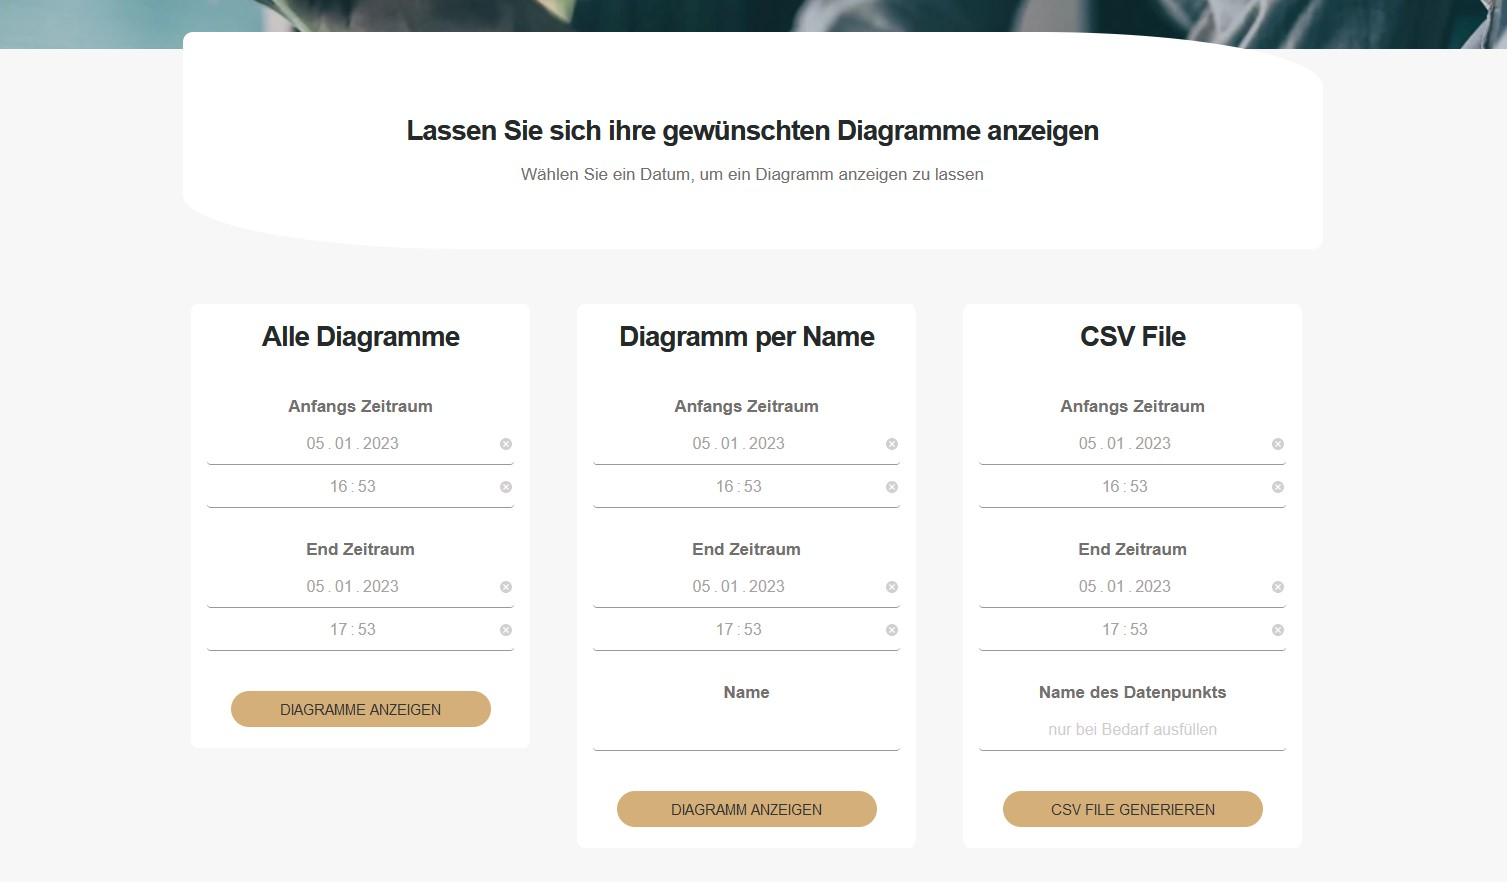
\includegraphics[scale=0.45]{pics/FlexLoggerWebsiteFormulare.jpg}
    \caption{Website Hauptseitenansicht}
    \label{fig:impl:FlexLoggerHauptseitenAnsicht}
\end{figure}

\begin{figure}
    \centering
    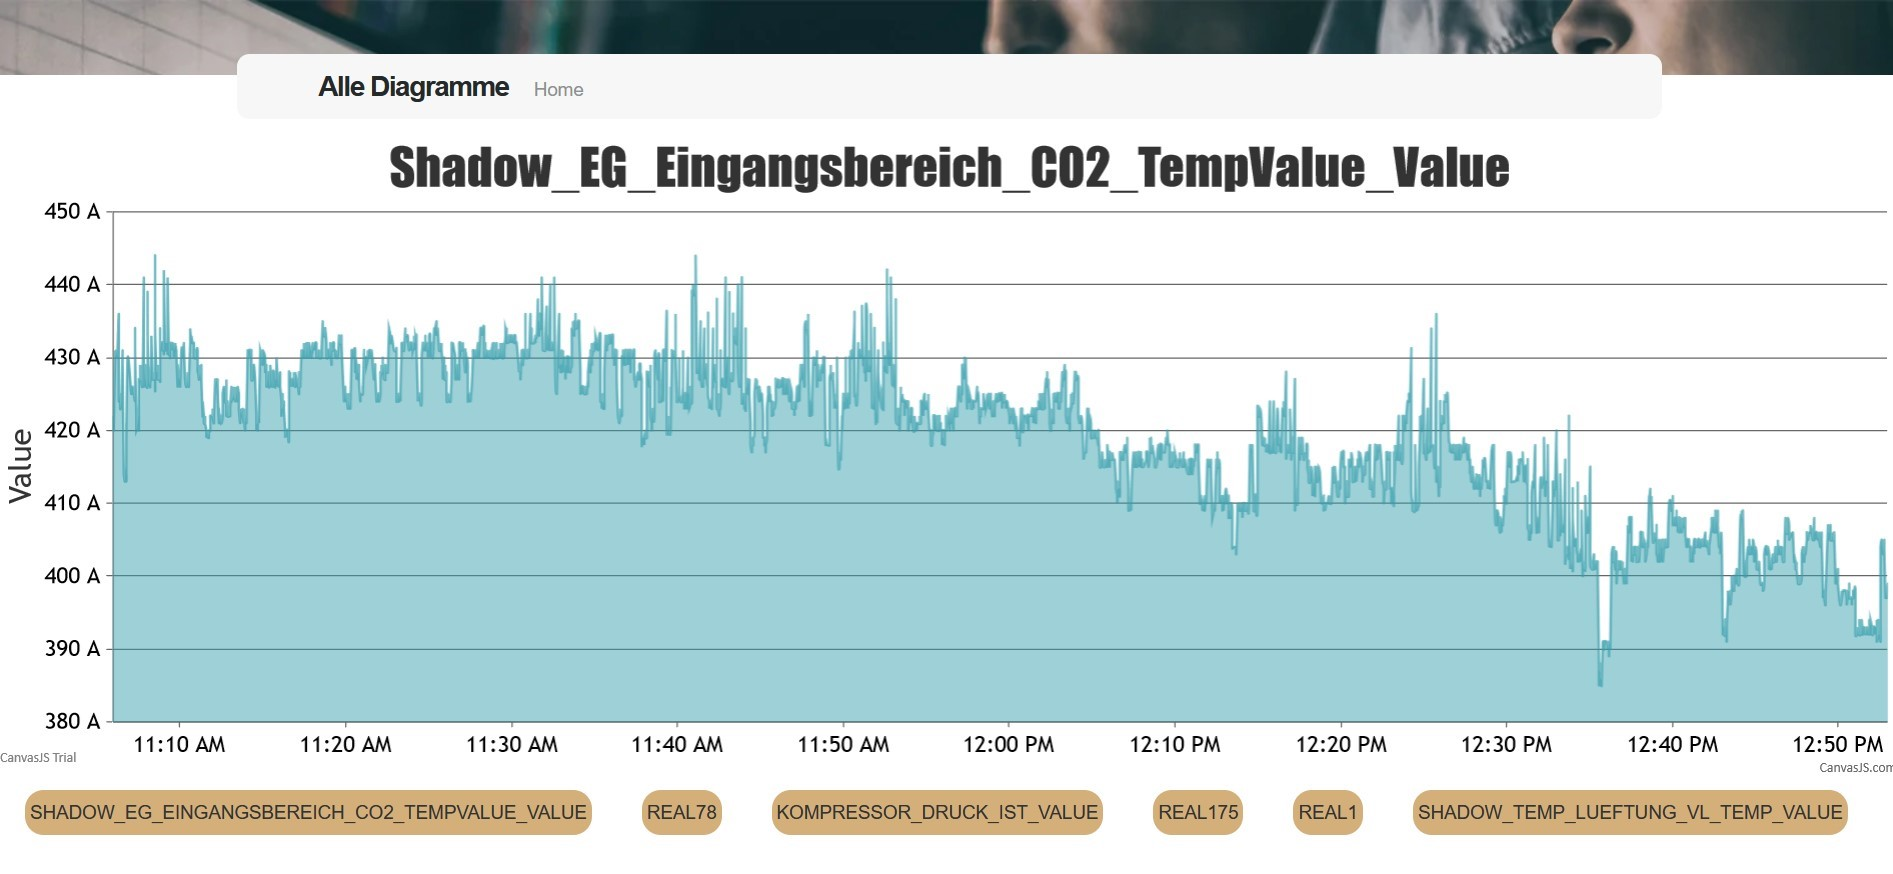
\includegraphics[scale=0.35]{pics/FlexLoggerWebsiteDiagramm.jpg}
    \caption{Website Diagrammansicht}
    \label{fig:impl:FlexLoggerDiagrammAnsicht}
\end{figure}

\subsubsection{App-Component}
In der TypeScript Klasse der App-Komponente wird ansich ein Titel definiert, dieser trägt in diesem Fall den Namen „flexloggerFE2“. Im HTML-File ist dabei ein Router-Outlet definiert. Durch dieses wird das Routing im Projekt ermöglicht. Das heißt jede Komponente wird praktisch in der App-Komponente angezeigt. In der app-routing-module Klasse werden alle Pfade des Projekts definiert. Dabei wird jeweils ein String als Pfad angeben, sowie eine Komponente definiert, zu welcher der Pfad führen soll. Zusätzlich wird bei den Modulen des Projekts ein RouterModule hinzugefügt, welches zusätzlich die Methode forRoot verwendet, in welchem die vorher definierten Routen als Parameter übergeben werden. In der app-module Klasse werden noch weitere Module hinzugefügt: 

\begin{compactitem}
    \item BrowserModule: Stellt einen Service zur Verfügung, mit welchem man eine Browser-app starten, sowie laufen lassen kann.    
    \item AppRoutingModule: Ermöglicht das Navigieren zwischen verschiedenen Komponenten.     
    \item HttpClientModule: Mithilfe dieses Moduls können Netzwerk Requests abgesetzt werden. Diese inkludieren GET, POST, PUT, PATCH und DELETE.    
    \item FormsModule: Durch dieses Modul können template-driven Forms erstellt werden.    
    \item ReactiveFormsModule: Mithilfe dieses Moduls kann ein reactiveForm verwenden. 
\end{compactitem}

\subsubsection{Home-Component}
Die ist die Haupt Komponente des Programms. In ihr werden 3 Formulare definiert, jedes davon hat eine andere Funktion. Im Konstruktor der Komponente werden verschiedenste Parameter übergeben:

\begin{compactitem}
    \item HttpService: Dies ist der Service, mithilfe dessen eine Server-Verbindung zum Backend aufgebaut werden kann.    
    \item Router: Mithilfe dieses in Angular eingebauten Features kann auf der Website zwischen den Komponenten gewechselt werden.        
    \item ActivatedRoute: Mithilfe dieses Parameters können Daten über Komponenten hinweg übergeben werden.    
    \item FormBuilder: Durch diesen Parameter können Reactive Formulare erstellt werden??
    \item ValidatorService: Wird später verwendet, um die Richtigkeit der Eingabe bei den Formularen zu garantieren.
\end{compactitem}

Im Konstruktor selbst, wird das heutige Datum sowie das heutige Datum plus einer Stunde gesetzt.
Um die Komponente zu initialisieren, wird in der ngOnInit()-Methode die initForms-Methode aufgerufen. Diese initialisiert alle 3 Formulare, indem sie die Variablen in den Formularen, sowie Validatoren setzt. Dabei werden bei den Variablen jeweils ein Standard-Wert gesetzt. Die gesetzten Validatoren überprüfen dabei, ob die Daten korrekte Eingaben in den Formularen sind. 

Weiteres findet man in der Komponente zwei Methoden, welche sich um das Routing kümmern. Diese kommen beim Klicken der Buttons der Formulare zum Einsatz, um die Komponente, welche angezeigt wird, zu wechseln. Die benötigten Daten werden dabei in der URL übergeben.

Die nachfolgende Methode ist für das Generieren sowie das Downloaden einer CSV-Datei zuständig. Zuallererst wird die checkCSV-Methode aufgerufen, in welcher überprüft wird, ob in dem ausgewählten Zeitraum Daten verfügbar sind.

Wenn die checkCSV-Variable als true gesetzt wurde, wird überprüft, ob der Namenparameter im Formular nicht leer ist. Trifft dies ein, wird mithilfe eines Timers und des Http-Service eine CSV-Datei generiert, welche alle Datenpunkte in dem richtigen Datumsbereich generiert. Nachdem das Generieren erfolgreich abgeschlossen wurde, wird der Download der Datei gestartet. Dieser Download wird mithilfe der window.open() Methode verwirklicht. Wenn der Namenparameter in dem Formular einen Namen enthält, so wird ein CSV-File generiert, welches nur die Daten eines Datenpunkts beinhält.

Wenn der Fall eintrifft, dass die checkCSV-Variable auf false gesetzt wurde, dann werden die Errors des Namenparameters auf true gesetzt. Dadurch wird unter dem Formular eine Fehlermeldung ausgegeben, um dem User eine Rückmeldung der Formulareingabe zu geben.

\subsubsection{Canvas-Chart-Component}

In dieser Komponente wird ein Diagramm erstellt, in welchem anschließend mithilfe von verschiedenen Buttons die gewünschten Daten angezeigt werden.  

Der erste wichtige Teil der Komponente ist das Erstellen der Diagramm Optionen. In diesen kann man verschiedenste Attribute eines Diagramms definieren: 

\begin{compactitem}
    \item animationEnabled: Stellt ein, ob beim ersten Anzeigen eines Diagramms jeder Punkt des Diagramms flüssig geladen wird, um ein dynamischeres Ergebnis zu erhalten.    
    \item title: Setzt den Titel fest, welcher als Überschrift über dem Diagramm stehen soll.          
    \item axisY: Legt den Titel der Y-Achse fest, diese Einstellung kann genauso auf der X-Achse getätigt werden.    
    \item data: Dies ist die wichtigste Einstellung der Diagramm Optionen. Sie legt den Typ des Diagramms fest (in diesem Fall ist es ein Liniendiagramm), die Farbe des Diagramms und setzt die Datenpunkte fest. Beim ersten Laden der Seite werden die Datenpunkte der X- und Y- Achse auf 0 bzw. den 01.01.1970 gesetzt. 
\end{compactitem}

Beim Laden der Seite wird zuerst im Konstruktor der Komponente eine Funktion namens onload() ausgeführt. Diese ist dafür zuständig, die erforderlichen Daten mithilfe des http-Service aus dem Backend zu bekommen. Zuerst werden hierfür die übergebenen Werte aus dem Formular mithilfe von Route Snapshots übergeben. Anschließend wird durch den http-Service eine getLogEntries-Methode aufgerufen, diese gibt die Werte zurück, welche das erforderliche Datum besitzen. Diese werden nun in einem Array gespeichert, um weiter verwendet zu werden.

Ion der nächsten Zeile des Konstruktors befindet sich ein Timer, welcher nach 1? Sekunde den darauffolgenden Code durchführt. In diesem Code wird zuallererst eine getFiles-Methode ausgeführt, diese gibt das vorher erstellte Array zurück. Das IF-Statement eine Zeile darunter garantiert, dass die Länge des Arrays nicht 0 beträgt, ansonsten wird die Fehlermeldung "Zu Ihrem ausgewählten Zeitpunkt wurden keine Daten gefunden." ausgegeben. Bei einem positiven Ergebnis des IF-Statements werden nachfolgend vier Methoden aufgerufen: 

\begin{compactitem}
    \item getListOfDatapointNames(): Diese Methode kümmert sich darum, eine Liste der Namen für die Buttons zu erstellen. Diese Buttons sind später dafür zuständig, zwischen den angezeigten Daten zu wechseln. 
    Um zu verhindern, dass der Name eines Datenpunkts öfters in der Liste vorkommt, wird am Beginn eine Boolean-Variable namens nameInList erstellt. Diese wird vorerst auf False gesetzt.
    Anschließend wird ein vorher initialisiertes Array auf ein leeres Array gesetzt, in welches danach die Namen hinzugefügt werden. Um alle Namen aus den Daten zu erlangen, wird eine for-Schleife verwendet, welche alle vorher erhaltenen Daten durchgeht. Der erste Name wird immer hinzugefügt, daher wenn die Länge des leeren Arrays 0 ist, wird der erste name hinzugefügt. Sonst wird eine weitere for-Schleife betreten, welche alle Elemente der List der Namen durchgeht. Wenn ein Element bereits vorhanden ist, wird die nameInList Variable auf true gesetzt. Später wird in einem weiteren If-Statement überprüft, ob diese Variable auf True oder False gesetzt ist. Bei einem False wird dabei der Name in die Liste hinzugefügt. Durch dieses Verfahren wird sichergestellt, dass kein Name doppelt in der Liste vorkommt und somit Buttons nicht doppelt angezeigt werden.    
    \item changeData()
    Hier werden die geänderten Daten in die Diagramm Optionen gespeichert. Um dies umzusetzen, wird als Parameter ein String namens filterString übergeben. Mithilfe diesem und einer For-Schleife werden alle Datenpunkte herausgefiltert, welche nicht den gewünschten Namen besitzen. Die richtigen Daten werden nun im Array dynamicLogLines gespeichert. Nach dem Aussortieren der Daten wird mit einem IF-Statement überprüft, ob die erste Stelle des dynamicLogLines nicht undefiniert ist. Wenn dies der Fall ist, wird der erste Datenpunkt, sowie der Titel in den Diagramm Optionen gesetzt. Danach werden die restlichen Datenpunkte mithilfe einer For-Schleife in den Diagramm Optionen gespeichert.               
    \item setChartOptions()
    Beim Aufrufen dieser Methode werden die Diagramm Optionen neu gesetzt. In diesem Fall wird der Titel, die Einheit und die Datenpunkte des Diagramms erneuert.        
\end{compactitem}

Anschließend wird eine Boolean-Variable namens showChart auf True gesetzt, wenn dieser Fall eintritt, wird auf der Website ein Diagramm angezeigt. 

\subsubsection{Canvas-Chart-Single-Component}
Die Komponente ist vom Aufbau her sehr ähnlich wie die Canvas-Chart-Komponente. Genau wie in der anderen Komponente werden zuerst einige Methoden im Konstruktor aufgerufen. Der größte Unterschied dabei ist, dass keine Buttonnamen erstellt werden, bzw. auch keine Buttons angezeigt werden. 

\subsubsection{HttpService}
Der Service ist dafür zuständig, die jeweiligen Daten aus dem Backend zu beschaffen. Zuerst wird ein String definiert in welchem die URL des Backend gespeichert ist. Im Konstruktor wird der sogenannte HttpClient als Parameter übergeben, er ist der Hauptakteur in der Klasse. Mithilfe von ihm kann eine Verbindung zum Server hergestellt werden. 

In dem Service befinden sich mehrere Methoden. Allgemein kann man sagen, dass man mit dem HttpClient jeweils einen GET-Request absetzt, welcher jeweils ein anderes Ergebnis liefert, je nachdem welche URL man als Parameter übergibt.

Die ersten beiden haben jeweils als Rückgabe-Paramater ein LogEntry Array. Beide geben die gesuchten Daten in einem bestimmten Zeitraum zurück, lediglich kann man bei der zweiten Methode noch einen Namen hinzufügen. Die Daten, welche die Zeiträume definieren, werden als Parameter in den Methoden übergeben. Die nächsten Methoden sind allesamt für das Downloaden eines CSV-Files verantwortlich. Dabei kümmern sich die ersten beiden um das Erstellen der CSV-Datei, die dritte ist für den eigentlichen Download verantwortlich. Um die CSV-Datei zu erstellen, werden wiederum die gewünschten Daten übergeben und anschließend wird daraus eine URL gebaut und ein GET-Request abgesetzt. Der einzige Unterschied zwischen den Methoden ist abermals ein zusätzlicher Name-Parameter. Die downloadCSV-Methode verwendet wie die anderen Methoden einen GET-Request, allerdings hat sie den weiteren Parameter responseType. Dieser ist notwendig, da innerhalb des Requests eine CSV-Datei gedownloadet wird und somit der Response-Type Array-Buffer definiert werden muss. 

\subsubsection{ValidatorService}
Der ValidatorService ist dafür zuständig, die Richtigkeit der Eingabe im Formular zu überprüfen. Wenn diese als nicht akzeptabel erkannt wurden, werden die Errors der Parameter auf true gesetzt, und somit eine Fehlermeldung ausgegeben.

Die match-Methode überprüft ob jedes eingegebene Datum als valide Eingabe akzeptiert werden kann. Dabei werden zuerst alle Controls des Formulars übergeben. Bei der ersten Überprüfung handelt es sich darum, ob das Startdatum hinter dem Enddatum liegt. Bei Bestätigung dieser Überprüfung werden die Errors mit dem Namen dateMustBeBigger aktiviert. Anschließend wird der Fall überprüft, wenn die beiden Daten gleich sind, die Zeiten sich allerdings unterscheiden, d.h. der Zeitraum am gleichen Tag stattfindet. Dies ist grundsätzlich erlaubt allerdings nur, wenn die Startzeit kleiner ist als die Endzeit. Wenn dies nicht der Fall ist, wird der Error timeMustBeBigger aktiviert.

\subsubsection{LogEntry Model}
Hier wird ein Model erstellt, welches den Namen LogEntry trägt, in diesem werden die Parameter dpId, value, unit und timeStamp definiert. Das Model wird dazu verwendet, um die vorher geloggten Daten aus der Datenbank weiterzuverwenden. 

\subsection{CanvasJS}
Mithilfe von CanvasJS, welche eine HTML5 und Javascript Charting library ist, wird das Anzeigen der Daten in Diagrammen ermöglicht. 

\begin{spacing}{1}
    \section{FlexTasks in der Flexcloud}\label{section:FlexTasks}
    \end{spacing}
\subsection{Was ist die Flexcloud?} \setauthor{Pouget Marcel}

Siehe Aufbau der Flexcloud: \ref{fig:impl:FlexcloudAnsicht}.

  \begin{figure}[h t]
    \centering
    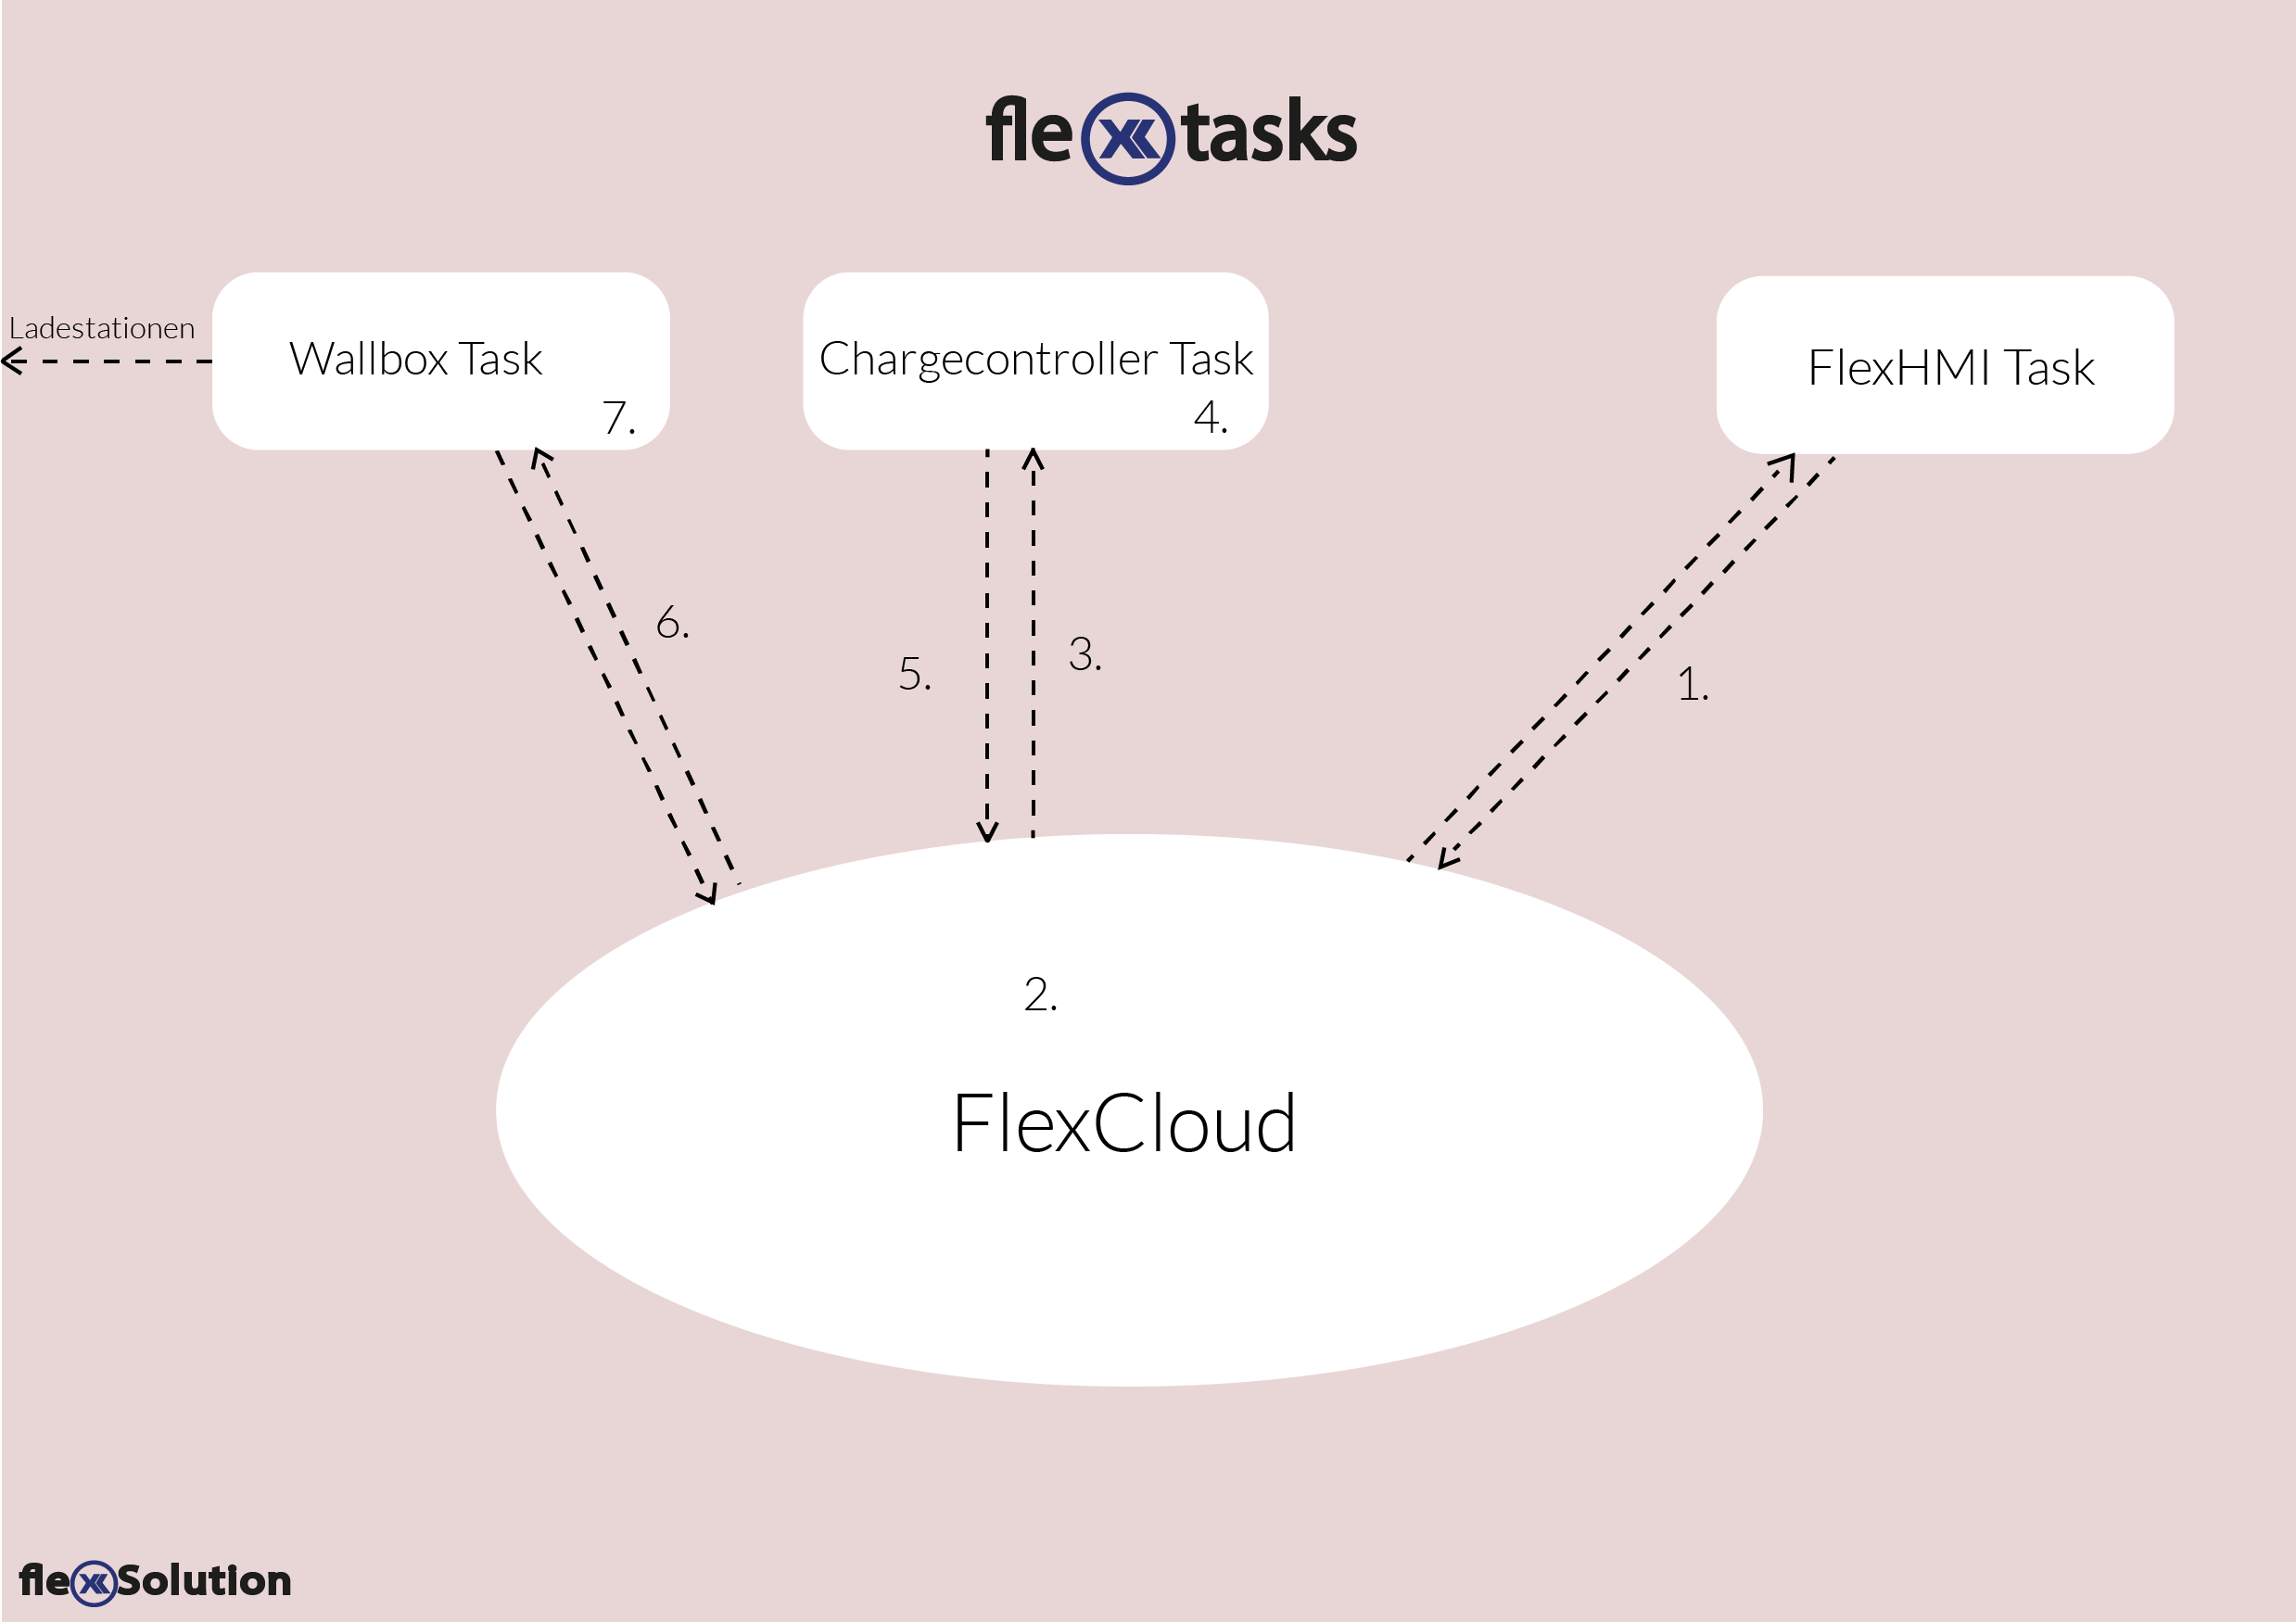
\includegraphics[scale=0.5]{pics/flexTasks2.png}
    \caption{Darstellung des Aufbaues}
    \label{fig:impl:FlexcloudAnsicht}
\end{figure}

Die Flexcloud, auch FlexcommunicationCloud genannt, ist eine Erfindung der Firma FlexSolution. Die Anwendung findet im Firmeneigenen Netzwerk statt, und ermöglicht es, viele kleine Microservices miteinander kommunizieren zu lassen. Die Hauptkomponente, der sogenannte FlexCore, wurde von den Mitarbeitern in der Sprache Java entwickelt. Mit der sogenannten Flexlib lassen sich die Anwendungen mit vielen weiteren kleinen Dependencies erweitern. Das wird vor allem dann benötigt, wenn z.B. eine Datenbankanbindung notwendig ist. Die Flexcloud besteht also aus lauter sogenannten Flextasks, welche verschiedene Aufgaben ausführen. Es zum Beispiel einen Task, der für die Ansteuerung der Lampen und Rollos zuständig ist. 
Ein weiterer Task, der für die HMI zuständig ist, verbindet die Flexcloud mit dem Browser. Die FlexcommunicationCloud ist auch für viele kleinere Anwendungen nützlich, da sich solche Microservices sehr schnell aufsetzen lassen. Man kann einzelne Tasks aufsetzen oder mehrere miteinander verbinden und kommunizieren lassen. Das hat den Vorteil, dass man wiederverwendbare Anwendungen entwickeln kann, welche nur grundlegende Funktionen erfüllen, aber von vielen Tasks gebraucht werden. So ist es z.B. in Planung, einen eigenen Modbus-Task zu implementieren, welcher nur dafür da ist, Befehle von anderen Tasks zu übernehmen und an eine USB-Schnittstelle weiterzuleiten. 
Damit die Tasks untereinander kommunizieren können, hat die Firma die sogenannten Datenpunkte (Datapoints) entwickelt. Sie dienen dazu, um zwischen einem oder mehreren Tasks Informationen oder Werte auszutauschen. Auch Funktionen-Aufrufe können durch solche Datapoints ermöglicht werden. Um durch Datenpunkte miteinander zu kommunizieren, müssen besagte FlexTasks mit den Project\_ID's verbunden werden. 
Wie man die Datenpunkte anlegen kann, was dabei wichtig ist und wie die Daten gemapped werden, wird im Kapitel \ref{Datenpunkte} beschrieben.
\subsection{Grundaufbau der Tasks}

\begin{compactenum}
    
    \item Pom.xml des Tasks editieren: Als erstes sollte die MainClass gesetzt werden. Dies folgt immer einem gewissen Schema. Die Klasse sollte im Package "eu.flexsolution.task." zu finden sein. Die GroupID ist dieselbe wie das Package der MainClass. In dem Fall ist es wieder "eu.flexsolution.task".  In der "artifactId" steht der Name des Tasks. Bei den Dependencies wird der "Flexsolution core", "log4j", "org.json". Eine weiter wichtige Sache ist das Einbinden des "Internal Snapshot Repository". Das ist der Ort, an dem der Flexsolution core und die Flexlib gepublished werden. Maven lädt dann beim Starten der Applikation die Dependencies von dem von der Firma bereitgestellten Server herunter, und fügt sie zur Applikation hinzu.   
    \item Das Anlegen der Main Klasse. Der erste Schritt ist, die Klasse "FlexTask" zu erweitern.  
    \begin{lstlisting}[language=java,caption=Example Element,label=lst:impl:foo]
        public class FlexTaskModbuswallbox extends FlexTask 
    \end{lstlisting}
    Dadurch werden einige Funktionen überschrieben, bei denen die meisten jedoch nicht verwendet werden. In der "public static void main" wird ein neues Objekt der Main Klasse erstellt.   
    \begin{lstlisting}[language=java,caption=Example Element,label=lst:impl:foo]
        new FlexTaskModbuswallbox();  
    \end{lstlisting}
    In der "initTask(){}" Methode kann dann die Hauptfunktion des Tasks implementiert werden. In den meisten Fällen werden hierfür Datenpunkte und andere Kommunikations-Methoden eingebunden. Mit Fertigstellung der App muss der Code mithilfe von Maven zu einem JAR-File kompiliert werden. 
    
    \item Linux-Maschine vorbereiten: Als erster Schritt ist es wichtig, ein Verzeichnis für den Task zu erstellen. In diese wird dann das .jar File kopiert. Da in der Firma mit "log4j" gearbeitet wird, muss hierfür noch ein Konfigurations-File angelegt werden. (siehe log4j File)  
   Da jeder Flextask eine Datenbank mit den für ihn zugehörigen Datenpunkten besitzt, muss dieses File auch erst angelegt und konfiguriert werden: im Verzeichnis ‘/var/flex/tasks/’ wird ein neuer Ordner mit dem Namen des Tasks angelegt. In diesem wird die Datei conf.db erstellt und folgende Tabellen hinzugefügt: 
    \begin{lstlisting}[language=java,caption=Example Element,label=lst:impl:foo]
        [Service]
        Type=simple
        ExecStart=/usr/bin/java -Xmx32m -Dlog4j.configurationFile=./log4j2.xml -jar /srv/tasks/CURRENT/modbuswallbox/modbuswallbox.jar
        Environment="TASKNAME=modbuswallbox"
        WorkingDirectory=/srv/tasks/CURRENT/modbuswallbox
        TimeoutStopSec=3
        Restart=always
        RestartSec=10
        Slice=flexTasks.slice
        [Install]
        WantedBy=default.target
    \end{lstlisting}
    \item Da jeder Flextask eine Datenbank mit den für ihn zugehörigen Datenpunkten besitzt, muss dieses File auch erst angelegt und konfiguriert werden: im Verzeichnis ‘/var/flex/tasks/’ wird ein neuer Ordner mit dem Namen des Tasks angelegt. In diesem wird die Datei conf.db erstellt und folgende Tabellen hinzugefügt: 
    \begin{compactenum}
        \item Device: besteht aus einer "ID" und einem Label. Im Falle des Gateways sind es 5 Geräte, für jede Wallbox eines. Das ist dafür gut, um Datenpunkte mit denselben Namen nutzen zu können, da man sie mithilfe der Deviceid unterschieden kann  
        \item DeviceParameter: Hier können wichtige Parameter gesetzt werden, die dann beim Starten eines Tasks mit der Methode "getNeededDeviceParameters(Map<String, ValueCheck> map)" ausgelesen werden können. Die Tabelle besteht aus einer ID, einer DeviceID, einem Wert und einem Label.  
        \item taskParameter: hier können wichtige Parameter für das System gesetzt werden. Meistens wird hier nur der Standard-Port 8150 gesetzt. Die Tabelle besteht aus einer Spalte für die ID, für Values und einer für Labels. Auch hier können beim Starten eines Tasks die Werte der DB ausgelesen werden. Hierfür verwendet man die Funktion "getNeededTaskParameters(Map<String, ValueCheck> map)".  
        \item datapoint\_valueMapping: Besteht aus einer Datapoint1\_id und Datapoint2\_id, einem Wert und einer Spalte für neue Werte (new\_Value). Dies ist dafür da, um zwischen zwei Datenpunkten die Werte zu synchronisieren oder gegebenenfalls mit new\_Value zu überschreiben  
        \item Datapoint: Herzstück der Datenbank. Hier werden die Datenpunkte angelegt \ref{Datenpunkte}. Die Tabelle besteht aus einer ID, einer device\_id, einem Label, einer "specificAddress", einem "specificDatatype", einem "specificStruct", einem Datentyp (datatype), Flags, einem Intervall, einem Threshold und einer Value. Für das Starten des Tasks ist diese Tabelle zu befüllen, jedoch ist sie unumgänglich, wenn man die Hauptfunktionen der Flexlib verwenden möchte  
        \item datapoint\_map: Diese Tabelle besteht aus einer datapoint1\_id, einer datapoint2\_id und einer Funktion. Diese Tabelle wird dazu verwendet, um Zwei Datenpunkte zu mappen (verknüpfen). 
        \item SystemParameter: Hier werden die wichtigsten Einstellungen für den Task selbst getroffen. Es gibt Einstellungen für den Namen des Tasks, den Port und man kann das keep\_Alive Signal einstellen. Außerdem gibt es die PROJECT\_ID, welche für das Verbinden mehrerer Tasks notwendig ist. Denn es können sich nur FlexTasks finden, welche dieselbe Project\_ID besitzen. Im Falle des Gateways werden die Tasks mit der ID "AUT, HMI, chargecontroller" verbunden. Das ist wichtig, um den einzelnen Tasks die benötigten Parameter zu übergeben. AUT ist in dem Fall die Haussteuerung, HMI ist der oben kurz beschriebene Flextask zur Veranschaulichung der Elemente und chargecontroller ist der auch schon beschriebene Controller für dieses Projekt.	 
    \end{compactenum}
    \item Wenn alle Pfade richtig benannt wurden, kann man im Verzeichnis einen symbolischen Link zu dem .jar-File machen. Das hilft bei der Entwicklung, da man bei einer Namensänderung nur den Link anpassen muss und nicht die angegebenen Pfade in den Konfigurations-Dateien.   
    \item Starten, stoppen bzw. überwachen kann man den Task mit "systemctl --user start / stop / restart / status FlextasName.service  
    \item Mit dem Command "tail -f /tmp/log/ FlextaskName.log" kann man in Echtzeit mitansehen, was Log4j in das File schreibt. Die Files werden alle in dem Verzeichnis "/tmp/log/" gespeichert, wenn sie nach einiger Zeit nicht mehr benötigt werden, werden sie komprimiert und in ein anderes Verzeichnis verschoben, um Platz zu sparen.   
\end{compactenum}


\begin{spacing}{1}
    \section{Datenpunkte}\label{section:datapoints}
    \end{spacing}
\subsection{Struktur eines Datenpunktes}\label{Datenpunkte}

Die Datenpunkte sind im Grunde alle gleich aufgebaut. Ein Datenpunkt (dp) besteht immer aus einer: 

\begin{compactitem}
    \item ID: kann nach Belieben benannt werden. Meist ein String, um den Nutzen zu veranschaulichen und die DP´s voneinander unterscheiden zu können. Die ID muss für jedes Device eindeutig sein.
    \item device\_id: gibt an, zu welchem Device der Datenpunt gehört. Ein Device kann in dem config.db-File hinzugefügt werden. Das dient dazu, um mehrere Datenpunkte mit derselben ID für mehrere Devices verwenden zu können. Die device\_id besteht immer aus einem INT. Um Datenpunkte nutzen zu können, muss mindestens ein Device angelegt werden. Die ID wird automatisch immer um eins erhöht. Im Normalfall ist schon ein Device mit der ID 1 und dem Label dev1 angelegt.
    \item Label: Hier kann man den Datenpunkt kurz beschreiben, um seine Funktion zu dokumentieren. Das wird dafür verwendet, um den Entwicklern das Verwalten der Datenpunkte zu vereinfachen.
    \item SpecificAddress: Ist meistens derselbe String wie die ID, kann jedoch auch etwas anderes sein. Wird dazu benötigt, um den Datenpunkt im Task anzulegen.
    \item SpecificDatatype: Hier kann ein String mitgegeben werden, um in einem Task einen Datentyp für den Datenpunkt festzulegen, bzw. zwischen Gruppen von Dp zu unterscheiden. Im Task für das Gateway wird der specificDatatype dafür genutzt, um zwischen Datenpunkten, die nur für Modbus zuständig sind, und den anderen Datenpunkten zu unterscheiden.
    \item Datatype: hier kann man angeben, welchen Datentyp die Value haben soll. Man kann hier zwischen "INT", "REAL", "BOOL" und "CMD" wählen.
    \item Intervall: Hier kann man ein Intervall angeben, mit welchem der Datenpunkt in die Flexcloud gepusht werden soll. Standardmäßig ist –1 eingestellt, was bedeutet, dass der Datenpunkt nur nach Anfrage des Tasks bzw. bei Änderung der Value gepublished wird.
    \item Value: Hier werden die Werte eines Datenpunktes gespeichert. Man kann in der conf.db Datei einen Standardwert angeben, doch meistens werden diese Werte in einem Task gesetzt bzw. ausgelesen. 
\end{compactitem}

\subsection{Anlegen eines Datenpunktes}


Um einen neuen Datenpunk in einem Task anzulegen, muss man sich zuerst auf die VM (Virtual machine),  auf welcher der Flextask sich befindet, verbinden. In dem Verzeichnis mit der conf.db Datei muss man mit SQLITE3 die Datei öffnen. Dort kann man dann mit einem insert bzw. Update Statement einen neuen Datenpunkt hinzufügen, aktualisieren oder löschen. 

\begin{lstlisting}[language=sql,caption=Example Element,label=lst:impl:foo]
    INSERT INTO datapoint VALUES ('Wallbox\textunderscore 1\textunderscore startCharching\textunderscore icon\textunderscore state',1,'','state\textunderscore [Wallbox\textunderscore 1\textunderscore startCharching\textunderscore icon]','','','INT',-1,-1,0.0,'');
\end{lstlisting}

\subsection{Nutzung eines Datenpunktes:}

Somit ist der Datenpunkt in der Datenbank angelegt und ready to use. Um nun in einem Flextask auf so einen Datenpunkt Zugriff zu haben, muss man ihn erstmal anlegen und die “SPECIFIC\_ADDRESS” angeben: 

\begin{lstlisting}[language=java,caption=Example Datapoint,label=lst:impl:foo]
    Datapoint datapoint = StaticData.datapoints.getDatapoint(Datapoints.DatapointField.SPECIFIC\textunderscore ADDRESS, "SPECIFIC\textunderscore ADDRESS\textunderscore DES\textunderscore DATENPUNKTES"); 
\end{lstlisting}

Nun hat man mehrere Möglichkeiten, wie man Daten aus dem Datenpunkt lesen kann: 
\begin{compactenum}
    \item Man ruft die Methode “setDatapointChangedCommand()” auf. Diese Methode überschreibt eine in der Klasse Flextask, und ist dafür da, um auf Änderungen des Datenpunktes zu hören.
    \begin{lstlisting}[language=java,caption=Example catapoint usage,label=lst:impl:foo]
        datapoint.setDatapointChangedCommand(new DatapointCommand() { 
            @Override 
            public DatapointResponse execute(DatapointResult result) { 
         
               System.out.println(datapoint.getValue()); 
                return new DatapointResponse(DatapointResponse.ResponseCode.OK); 
            } 
        }); 
    \end{lstlisting}
    Diese Methode gibt bei jeder Änderung des Wertes den neuen Wert in der Konsole aus. Hier kann man den Wert speichern, andere Methoden ausführen, oder sonst alles machen, was man in einer Methode machen könnte. 

    \item Man kann jederzeit im Code "datapoint.getValue()" aufrufen. Mit dieser Methode bekommt man immer den jetzigen Wert des Datenpunkts zurück.   
    \item Wie schon in den vorhergegangenen Kapiteln erwähnt, kann man über alle Datenpunkte jedes Device iterieren, und je nach Bedingung ein DatapointCahngedCommand anhängen. Dies bewirkt, dass eine Methode immer dann aufgerufen wird, wenn sich einer der Datenpunkte ändert. Mit der ID der einzelnen Devices kann man dann auf die SpecificAddress zugreifen, und die einzelnen Fälle mit einem switch Statement abdecken. 
    \begin{lstlisting}[language=java,caption=Example multible datapoint usage,label=lst:impl:foo]
        for (Device dev : StaticData.devices.getDevices()) { 
    for (Datapoint dp : StaticData.datapoints.getDatapoints(dev.getId())) { 
        if (!dp.getSpecificDataType().isEmpty()) { 
            dp.setDatapointChangedCommand(dpCmd);                 //!!! 
        } 
    } 
} 

 

DatapointCommand dpCmd = new DatapointCommand() { 
      @Override 
    public DatapointResponse execute(DatapointResult datapointResult) { 
 
        int deviceID= datapointResult.getDeviceId();  
        switch (datapointResult.getDpId()) { 
            case "datapoint\textunderscore example\textunderscore id": 
                System.out.println(datapointResult.getValue() + " " + deviceID ); 
                 break; 
                    } 
        return new DatapointResponse(DatapointResponse.ResponseCode.OK); 
    } 
}; 

    \end{lstlisting}
    In diesem Beispiel werden die DeviceID und der aktuelle Wert des Datenpunktes, welcher sich geändert hat, ausgegeben.
\end{compactenum}

Mit “datapoint.setValue(value)” kann man einem Datenpunkt einen neuen Wert zuweisen. Dieser wird dann automatisch in die FLexcloud gepublished, und kann von einem anderen Task abgefangen werden.  


\subsection{Datapoint mapping}

Um zwei Datenpunkte von zwei verschiedenen Tasks zu mappen, und somit Daten zu übertragen, muss man einen Eintrag in der “datapoint\_map” hinzufügen. Um die Daten zu empfangen, muss man die conf.db des zweiten Tasks aktualisieren. Zu beachten ist, dass das Mapping nur bei dem Task gemacht werden muss, welcher die Daten bekommen soll. Man verbindet also den Datenpunkt eines anderen Tasks auf einen eigenen Datenpunkt. Wichtig dabei ist, dass man bei der “datapoint1\_id” zuerst das Label des Devices, zu welchem der Datenpunkt gehört, und anschließend die ID des ersten Datenpunkt angibt. “datapoint2\_id” wird zuerst der Name des anderen Tasks angegeben, dann das Label des Devices, und anschließend die ID des Datenpunktes. 

 

Beispiel: Ich möchte von dem Flextask “modbuswallbox”, welcher in dem Projekt als das Gateway bezeichnet wurde, den Wert der Ladedauer der ersten Wallbox zum “chargecontroller” schicken. In dem Task “modbuswallbox” muss dafür ein Device mit dem Label “wb1” und ein Datenpunkt mit der ID “ladedauer\_wb1” angelegt werden. Wird nun im Code auf diesen Datenpunkt was gepublished, sieht man “modbuswallbox.wb1.ladedauer\_wb1”. Damit die Daten jetzt auch ankommen, muss im Task für den Charge-controller ein Datenpunkt mit der ID “ladedauer\_wb” angelegt werden. In die “datapoint\_map” Tabelle muss dann bei der “datapoint1\_id” das Device und der Datenpunkt angegeben werden, und bei der “datapoint2\_id” zuerst der Task Name, das Device und dann der Datenpunkt, der die Daten pulished. 

\begin{lstlisting}[language=sql,caption=Example Element,label=lst:impl:foo]
    dev1.ladedauer_wb                       modbuswallbox.wb1.ladedauer_wb1
\end{lstlisting}

\begin{spacing}{1}
    \section{Modbus}\label{section:modbus}
    \end{spacing}
\label{ModbusErklärung} \setauthor{Pouget Marcel}
Um die Art der Kommunikation zwischen den Wallboxen, der PV-Anlagen, den Janitza Klemmen und dem Raspberry PI zu verstehen, muss man sich erstmals mit der Übertragung an sich beschäftigen.
\subsection{7 Schichten OSI-Modell} \label{OsiModell}

Mit dem Open System Interconnection Reference Model (kurz OSI-Referenzmodell) lässt sich am besten beschreiben, wie und auf welchen Ebenen die Daten übertragen werden.  Kurz zusammengefasst ist es ein Modell, das die Kommunikation in einem Netzwerk in sieben Schichten unterteilt. Die Entwicklung, welche seit 1983 als Standard veröffentlicht wird, begann bereits 1977.  Der Fokus der Entwicklung war es, ein Modell zu erschaffen, mit welchem sich die Kommunikation zwischen Systemen, auch innerhalb eines Netzwerkes, beschreiben lassen. Es gibt dabei sieben Schichten, auf welche sich unterschiedliche Übertragungsarten abspielen. 

Die sieben Schichten des OSI-Modells sind:  

\begin{compactenum} 
    \item Die Bitübertragungsschicht ist die unterste Schicht. Die physische Schicht umfasst die Hardware, die zur Übertragung von Daten über das Netzwerk verwendet wird, wie zum Beispiel verschiedene Kabel (wie Netzwerkkabel, Serielle Verbindungen), Hubs, Switches und Router. Außerhalb eines Netzwerkes könnte die physische Schicht auch der Rauch sein, mit dem Rauchzeichen übermittelt werden, oder die Luft, wenn es um Morsezeichen geht. Im Grunde alles, durch was sich verschlüsselte Nachrichten übermitteln lassen.  
    \item Ein wichtiger Bestandteil eines Netzwerkes ist die Datenübertragungsschicht. Diese ist verantwortlich für die Übertragung von Datenpaketen von einem Gerät zu einem anderen. Hierbei spielt die MAC-Adresse eine wichtige Rolle, da sie dazu verwendet wird, um einzelne Geräte in einem Netzwerk zu identifizieren. Im Gegensatz zur IP-Adresse besteht die MAC-Adresse aus 48 Bit. Die MAC-Adresse wird in hexadezimaler Form dargestellt, ein Beispiel dafür wäre 00-1D-60-4A-8C-CB. Dabei werden stets zwei Bytes zusammengefasst und durch einen Bindestrich oder durch einen Doppelpunkt getrennt. Die ersten drei Bytes der MAC-Adresse sind die Kennung des Herstellers, welche auch als “OUI” bekannt ist. Die restlichen drei Bytes werden von dem jeweiligen Hersteller vergeben und dienen dazu, einzelne Geräte voneinander zu unterscheiden. Das ermöglicht eine eindeutige Identifizierung im Netzwerk und verhindert, dass doppelt MAC-Adressen im Netzwerk vorkommen. Jeder Hersteller muss hierfür ein entsprechendes Schema überlegen, um die letzten drei Bytes einer MAC-Adresse eindeutig zu vergeben.     \cite{wieisteineMacaufgebaut}
    \item Die Netzwerkschicht ist für die Vermittlung von Datenpaketen zwischen Netzwerken verantwortlich und verwendet IP-Adressen, um Geräte im Internet zu identifizieren. \cite{ipAddress} Die klassischen IP4 Adressen bestehen, wie der Name vermuten lässt, aus 4 Bytes und einer Subnetmask. Diese ist dafür da, um die Adresse in zwei Teile zu unterteilen. Der vordere Teil repräsentiert dabei immer den Netzwerkteil und der hintere die Computer ID. Für private Netzwerke gibt es reservierte Bereiche. 10.0.0.0/8, was vor allem in großen Firmen benötigt wird, da es 16.777.216 mögliche Adressen gibt. Im Heimnetz sieht man vor allem 172.16.0.0/12 und 192.168.0.0/16. Bei diesen IPS kann man in einem Netzwerk viel weniger Geräte benutzen. Bei der 172.16.0.0/12 sind es immerhin noch 1.048.576 mögliche Geräte, und bei der letzten Möglichkeit nur noch 65.536. Deswegen findet man in privaten Haushalten diese am häufigsten. Ein klassisches Beispiel wäre: 192.168.0.100/16.   
    \item Die Transportschicht ist für die Übertragung von Daten zwischen Endgeräten verantwortlich und sorgt dafür, dass die Übertragung fehlerfrei erfolgt. Auf dieser Schicht kommen vor allem die Protokolle TCP und UDP zum Einsatz. TCP ist dafür da, um mit Hilfe einer Prüfsumme zu gewährleisten, dass alle Daten richtig bei dem Empfänger ankommen. UDP hingegen ist ein auf Geschwindigkeit angelegtes Protokoll, bei dem es auch vorkommen darf, wenn ein paar Bits verloren gehen,   
    \item Die Sitzungsschicht ist für die Verbindungsaufnahme und -beendigung zwischen Endgeräten verantwortlich und sorgt dafür, dass die Übertragung ordnungsgemäß abläuft.  
    \item Die Darstellungsschicht ist für die Umwandlung von Daten zuständig. Die Daten werden in ein für die Übertragung geeignetes Format umgewandelt, und sorgt dafür, dass die Daten in der richtigen Form, also richtig formatiert, an ihr Ziel gelangen. Auch Kompression und Verschlüsslungen gehören zu dieser Schicht.   
    \item Die Anwendungsschicht ist die oberste Schicht und ist dafür verantwortlich, um mit den Anwendungen kommunizieren zu können. Diese werden auf den Endgeräten ausgeführt. Über diese Schicht wird die Verbindung zu den unteren Schichten hergestellt. Hier werden vor allem Applikationen verwendet, mit denen man Daten austauschen kann. Typische Beispiele sind Webbrowser, E-Mail-Programme oder Nachrichtendienste.  
\end{compactenum}\cite{ISO/OSI-Referenzmodell}


Das OSI-Referenzmodell hilft, die Kommunikation in einem Netzwerk zu beschreiben und zu verstehen, indem es die verschiedenen Aspekte der Netzwerkkommunikation in logische Schichten unterteilt. Dies ermöglicht es, Netzwerkprotokolle zu standardisieren und die Kompatibilität von Geräten und Software in verschiedenen Netzwerken zu gewährleisten. 

\begin{figure}[h t] \cite{7schichtenModell}
    \centering
    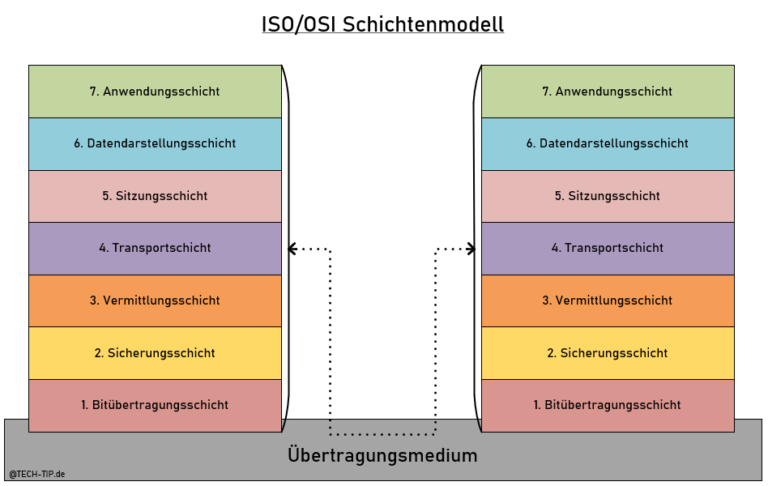
\includegraphics[scale=0.5]{pics/ISO-OSI-Modell-768x486.png}
    \caption{Das 7 Schichten OSI/ISO Modell}
    \label{fig:impl:Wallbox7schichtenmodell}
\end{figure}


\subsection{Modbus}\label{modbusprotokoll} \setauthor{Pouget Marcel}

Modbus ist ein Protokoll, welches 1979 entwickelt wurde, und vor allem in der Industrie große Bedeutung hat. Es ermöglicht eine Kommunikation zwischen automatisierten Maschinen, und wurde damals als Protokoll auf der Anwendungsebene implementiert, das Daten über die serielle Schicht übertragen soll. Das Protokoll gehört mittlerweile zu den Industriestandards, und wird vor allem in der Automatisierungstechnik gerne benützt. Mittlerweile hat sich Modbus weiterentwickelt, so dass es mehrere Implementierungen gibt. Der Datenaustausch ist mittlerweile über TCP/IP, seriell oder über das 'User-datagram-protocol', kurz UDP, möglich.
\cite{ModbusgrundlagenKubunu} \cite{modbuskubunu}

\subsection{Das Modbus Protokol}
Modbus ist ein sogenanntes request-response Protokoll, welches eine 'Master-slave' Beziehung nutzt. In so einer 'Master-slave' Beziehung funktioniert die Kommunikation immer paarweise – ein Gerät schickt eine Anfrage an einen 'Slave', und wartet auf eine Antwort. Der Master ist dabei für jede Interaktion verantwortlich. Der Master ist normalerweise ein einfaches HMI (human machine interface), oder ein 'Supervisory Control and Data Acquisition (SCADA) system'.  Der Slave ist meistens ein Sensor, eine Messklemme, ein programmable logic controller (PLC) oder ein Interface. Der Inhalt der Anfragen und Antworten sowie die Netzwerkschichten, über die diese Nachrichten gesendet werden, werden von den verschiedenen Schichten des Protokolls definiert. 
\cite{modbusoverserial}
\subsection{Die verschiedenen Layer des Modbus Protokoll }
In der ersten Implementierung war Modbus ein einzelnes Protokoll, welches auf Serielle Protokolle aufbaut, es konnte also nicht in mehreren Schichten aufgeteilt werden. (Modbus RTU) 
Über einen längeren Zeitraum wurden neue Implementierungen vorgestellt, um entweder das serielle Paketformat zu ändern oder die Verwendung von TCP/IP- und UDP-Netzwerken (User Datagram Protocol) zu ermöglichen. TCP, Remote Terminal Unit (RTU) und ASCII sind die drei am häufigsten verwendeten ADU-Formate. RTU- und ASCII-ADUs werden traditionell über eine serielle Verbindung verwendet, während TCP über zeitgenössische TCP/IP- oder UDP-IP-Netzwerke verwendet wird. 

\subsection{Aufbau des Modbus-Protokolls}
Am Anfang ist es wichtig zu erwähnen, dass jeder einzelne Teilnehmer (Slave) eine sogenannte Slave Id besitzt. Diese muss in einem 'Netzwerk' eindeutig identifizierbar sein, und kann je nach Hersteller fest vergeben, automatisch konfiguriert oder frei wählbar sein. Die Adresse 0 ist für den Master reserviert. Die einzelnen Teilnehmer können die Adressen von 1 bis 247 annehmen, da die Adressen von 248 bis 255 reserviert sind. Die Daten von den Slaves sind in sogenannten Registern gespeichert. Diese sind immer 16 Bit groß.  

Das Protokoll Modbus überträgt die Daten in binärer Form. Das führt dazu, dass man die Daten nicht direkt auswerden kann, sondern eine Möglichkeit des Parsens braucht, um auf die ursprünglichen Werte zu kommen. Vorteil ist jedoch, dass dadurch eine großer Datendurchsatz ermöglicht wird. 

 

Soll nun ein Paket über Modbus geschickt werden, muss man zuerst ein paar variablen Einstellungen treffen. So kann die Baudrate (Bitrate) oft frei gewählt werden (solange sie nicht von dem Hersteller festgelegt wurde, wie es bei den Wallboxen der Fall war). Außerdem gibt es sogenannte 'Stopbits', welche bei jedem Hersteller anders konfiguriert sind. Die Defaultwerte sind dafür 1 oder 2 Bits. 

 

Vor und nach jedem gesendeten Paket gibt es eine Sendepause (Wartezeit) von mindestens 3.5 Zeichen. Da ein Zeichen eine Länge von 11 Bit besitzt, hängt die Wartezeit von der Bitrate ab. Dabei ist zu beachten, dass vor allem bei einer niedrigen Übertragungsrate es sehr wichtig ist, diese Zeit genau einzuhalten, da es sonst zu Überschneidungen und zu Datenverlusten kommen würde.  

Nach der Pause fängt das Paket mit der Adresse des jeweiligen Slaves an. So kann jeder Teilnehmer direkt auf sein Packt reagieren. Bei jeder Antwort wird die Adresse zurückgesendet, damit der Master das Paket zuordnen kann. Die Adresse ist immer 8 Bits lange, und kann somit 256 Zustände einnehmen (ausgeschlossen sind die oben beschriebenen vordefinierten Adressen) 

Das nächste Byte enthält die Information über die Funktion. Folgende sind in der Produktion wichtig: \ref{tab:functionsfromModbus}

\begin{table}[h t]  
    \small
    \begin{tabular}{|l|l|}
    \hline
    
    Code & Description                                                         \\ \hline
    1    & \begin{tabular}[c]{@{}l@{}}Read \\ coils\end{tabular}               \\ \hline
    2    & \begin{tabular}[c]{@{}l@{}}Read \\ discrete\\  Inputs\end{tabular}  \\ \hline
    3    & \begin{tabular}[c]{@{}l@{}}Read \\ discrete\\  Inputs\end{tabular}  \\ \hline
    4    & Read Input Registers                                                \\ \hline
    5    & \begin{tabular}[c]{@{}l@{}}Write \\ single\\  Coil\end{tabular}     \\ \hline
    6    & \begin{tabular}[c]{@{}l@{}}Wirte \\ single\\  Register\end{tabular} \\ \hline
    7    & Read Exception Status (nur für serielle Übertragung)                \\ \hline
    \end{tabular}
    \caption{Die verschiedenen Functions von Modbus}
    \label{tab:functionsfromModbus}
\end{table}\cite{modbuswiki}

Bei der Kommunikation mit den Wallboxen wurde nur die Funktion 4 und 6 benutzt, um die Register auszulesen und neu zu beschreiben.   

Nach der Funktion kommen die eigentlichen Daten des Paketes. Diese bestehen immer aus einem Register. Je nach Funktion kommen noch andere Werte hinzu, zum Beispiel der Wert, den man auf ein Register schreiben möchte. Ein Register lässt sich hier sehr gut mit einer Adresse in dem jeweiligen Device vergleichen. Dort stehen nämlich die Daten des Gerätes bzw. dort können Werte gesetzt werden. Die Daten können dabei beliebig groß sein.  

Der CR-Check am Ende ist eine Prüfsumme des Paketes, um die Gültigkeit der Daten zu überprüfen. Diese Überprüfung ist vor allem bei der seriellen Kommunikation sehr wichtig, da es immer wieder zu Differenzen kommen kann, wo Daten verloren gehen und das Paket unvollständig ankommt. 
\ref{tab:modbusprotokollaufbautabelleRTU}

 \begin{table}[h t] 
    
    \small
    \begin{tabular}{|l|l|l|l|l|l|}
    \hline
    Start                        & Adresse & Funktion & Daten  & CR-Check & Ende                        \\ \hline
    Wartezeit  & 1 Byte  & 1 Byte   & n Byte & 2 Byte   & Wartezeit \\ \hline
    \end{tabular}
    
    \caption{Der Aufbau eines Modbus RTU Paketes}
    \label{tab:modbusprotokollaufbautabelleRTU}
 \end{table}

\subsection{Unterschiede zwischen Modbus TCP und RTU}

Die Modbus-Kommunikation über TCP ist der über RTU sehr ähnlich. Der größte Unterschied ist, wie der Name schon erraten lässt, hier wird das Paket über TCP verschickt. Die ganze Datenübertragung läuft über den Port 502, und der Master ist immer über eine IP-Adresse erreichbar. Es gibt noch folgende Unterschiede am Paket selber:  

Jedes Paket hat eine Transaktionsnummer, die immer 16 Bits lang ist. Danach kommt, mit derselben Länge, ein Protokollkennzeichen, welches immer gleich ist (0x0000). Der nächste Abschnitt beschreibt, wie viele Bytes noch folgen werden. Dieser Bereich ist immer um 2 Byte größer als die tatsächliche Anzahl der Bytes.  Die Länge der Adresse, der Funktion und der Daten ist dieselbe wie bei Modbus TCP. \ref{tab:allgemein:modbusprotokollaufbautabelle}

\begin{table}[h t]
    \tiny
    \begin{tabular}{|l|l|l|l|l|l|}
    \hline
    Transaktionsnummer & Protokollkennzeichen  & Zahl der noch folgenden Bytes & Adresse & Funktion & Daten  \\ \hline
    2 Byte             & 2 Byte (immer 0x0000) & 2 Byte (n + 2)                & 1 Byte  & 1 Byte   & n Byte \\ \hline
    \end{tabular}
    \caption{Der Aufbau eines Modbus TCP Paketes }
    \label{tab:allgemein:modbusprotokollaufbautabelle}
   % \cite{modbuserklärunginnovations}
\end{table}




\subsection{Modbus RS485 vs RS232} \setauthor{Pouget Marcel}
Es gibt bei Modbus RTU noch weitere Unterteilungen, welche sich in der physikalischen Ebene unterscheiden. Die größten Unterschiede sind dabei die Länge der Kabel, welche verwendet werden, die Art, wie die Teilnehmer mit dem Master verbunden sind, und der Pegel, welcher in den Leitungen herrscht.   

Bei Modbus 485 ist aufgrund der physischen Bauweise eine viel größere Länge der Kabel möglich. Während bei Modbus 232 meist nur eine Kabellänge von 10-15 Metern wirklich gut funktioniert, kann bei RS485 eine Länge von bis zu 1200 Metern erreicht werden.   

Auch der Signalpegel ist ein großer und wichtiger Unterschied. Während RS485 differentielle Signale nutzt, die zwischen positiven und negativen Spannungen schwanken, nutzt RS232 eine Spannung von 3V.   

Ein weiterer wichtiger Punkt ist die Verkabelung der einzelnen Teilnehmer. Während bei Modbus RS232 eine Punkt zu Punkt Verkabelung verwendet wird, sind die Slaves bei RS484 alle an denselben zwei Kabeln angeschlossen (siehe Abbildung Bild). Ein weiterer, wichtiger Punkt ist der Abschlusswiderstand, den man am Ende jeder Leitung braucht. Dieser dient dazu, um Interferenzen zu verringern, und so Störungen im System zu eliminieren.  
\cite{UnterschiedeinModbus}



\begin{figure}[h t] \cite{modbusaufbauimg}
    \centering
    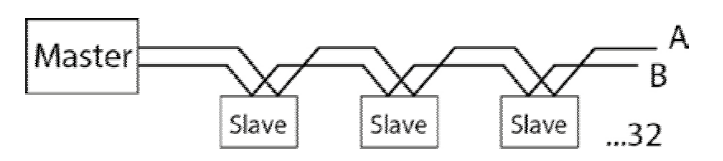
\includegraphics[scale=0.5]{pics/RS485-Schnittstelle-11.png}
    \caption{Aufau eines Modbus-Netzwerkes}
    \label{fig:impl:WallboxModbusnetzwerk}
\end{figure}

\subsection{Modbus tools + libraries} \setauthor{Pouget Marcel}

Es gibt viele tools, mit denen man über einen USB zu Modbus Konvertern Modbus-Register auslesen kann. Für diese Arbeit wurden hauptsächlich die Programme 'QModMaster' und 'Hercules' verwendet. Es handelt sich bei beiden um kostenlose Programme.  \ref{fig:impl:QmodMasterverview}

\begin{figure}[h t] 
    \centering
    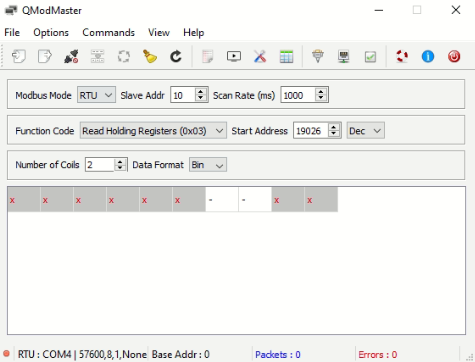
\includegraphics[scale=0.7]{pics/QmodMasterverview.png}
    \caption{Overview von QModMaster }
    \label{fig:impl:QmodMasterverview}
\end{figure}


In QModMaster kann man beim Modbus-Modus zwischen dem Modus RTU und TCP wechseln, da das Programm beides unterstützt. Unter der Slave Adresse kann man den gewünschten Teilnehmer auswählen. Hier ist es in dem Beispiel der Slave mit der ID 10. Mit der Scan-Rate kann man ein Intervall einstellen, mit welchem das Tool den Port abfragt.   

Bei dem Abschnitt 'Function Code' kann man auswählen, welche Funktion \ref{tab:functionsfromModbus} ausgeführt werden soll. Die Start-Adresse ist das Register, welches beschrieben oder ausgelesen werden soll. Hier kann man auch noch angeben, auf welche Art die Daten übermittelt werden sollen. Es gibt die Möglichkeit für Binär-, Dezimal- und Hexadecimal-Zahlen. 

Die 'Number of Coils' sagt an, wie viele Register auf einmal ausgelesen / beschrieben werden sollen, da bei manchen Geräten die Werte für ein Register zu groß sind (über 65536). In solchen Fällen werden die Daten je nach Hersteller in 2 oder mehreren Registern abgespeichert. Sollte dies der Fall sein, ist es aber immer vom Hersteller dokumentiert.   

Der untere Bereich ist das Ergebnis, welches der Slave zurücksendet. Hier kann man auch auswählen, in welcher Form die Daten angezeigt werden sollen. Ganz unten sieht man noch eine Zusammenfassung der Einstellungen, wie viele Packages gesendet wurden und wie viele davon fehlerhaft waren.   

\begin{figure}[h t] 
    \centering
    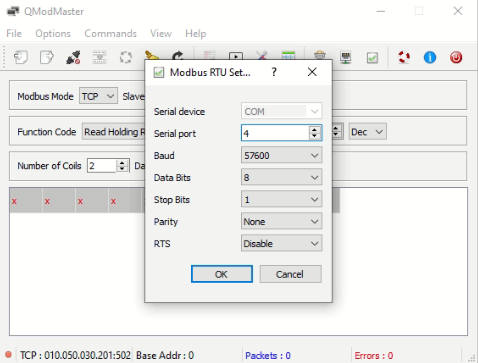
\includegraphics[scale=0.7]{pics/Settingsforqmodmaster.png}
    \caption{Einstellungen für Modbus RTU}
    \label{fig:impl:Settingsforqmodmaster}
\end{figure}


\ref{fig:impl:Settingsforqmodmaster} Hier kann man die Werte der Parameter einstellen. Das 'Serial-device' ist in diesem Fall der USB-Port des Computers, und der 'Serial-port' ist der Steckplatz, in welchem der Modbus-Konverter steckt. Falls man den Port des Adapters nicht kennt, findet man diesen in Windows unter den verbundenen Geräten im Gerätemanager.  

'Baud' ist die Konfiguration für die Baudrate. Diese muss mit den Angaben des Herstellers übereinstimmen.  

Data-Bits beschreibt die Länge des Protokolls. Dieser Wert ist auch im Datenblatt des jeweiligen Gerätes zu finden.  

Die Stop-bits findet man auch in den Angaben des Herstellers. Der Wert beträgt meist 1 oder 2 Bits. Parity und RTS sind meist disabled, können aber bei Bedarf auch konfiguriert werden.  

\begin{figure}[h t] 
    \centering
    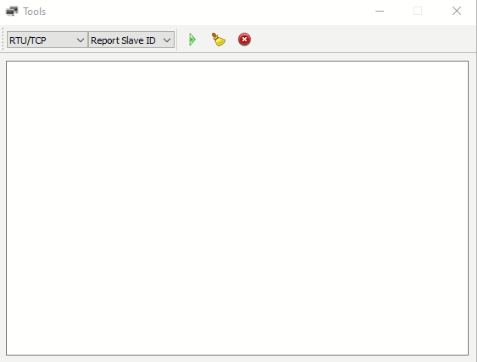
\includegraphics[scale=0.7]{pics/ToolsQModbusMaster.png}
    \caption{Einstellungen für Modbus RTU}
    \label{fig:impl:ToolsQModbusMaster}
\end{figure}

Außerdem gibt es einen Monitor, auf welchem man genau die einzelnen Abfragen des Tools nachvollziehen, und abspeichern kann. Auf der \ref{fig:impl:ToolsQModbusMaster} findet man noch weitere Tools, die man in Verbindung mit Modbus verwenden kann.  


Wenn man mit QModbusMaster eine Modbus TCP Verbindung aufbauen möchte, muss man den Mode auf TCP stellen. Die Einstellmöglichkeiten sind fast identisch zu der Modbus RTU Verbindung, hier muss man lediglich die Unit ID anstatt der SlaveID einstellen, jedoch ist es derselbe Wert. \ref{fig:impl:QmodbusMasterTCP}

\begin{figure}[h t] 
    \centering
    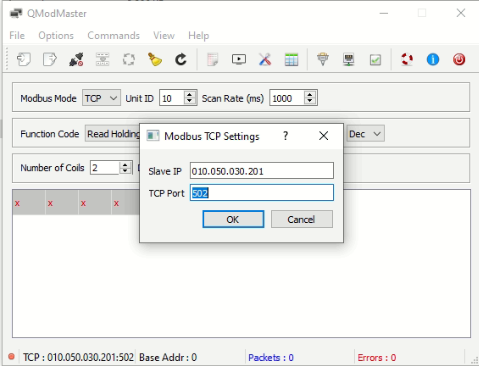
\includegraphics[scale=0.7]{pics/QmodbusMasterTCP setting.png}
    \caption{Einstellungen für Modbus RTU}
    \label{fig:impl:QmodbusMasterTCP}
\end{figure}

Hier ist der größte Unterschied zu der Modbus RTU. Denn anstatt der ganzen Parameter für die serielle Übertragung, wird hier nur der Port und die IP-Adresse des Teilnehmers eingestellt. Der Port ist standartmäßig 502. Sollte ein anderer Port konfiguriert sein, wird dies immer in der Dokumentation des Herstellers angegeben. 

 \subsection{Modbus Librarys für Java }

 Es gibt viele Librarys für Modbus, doch viele von ihnen bauen auf eine Schnittstelle auf, welche in C++ geschrieben wurde. Für das Projekt kam aber aufgrund der Firmenarchitektur nur ein Dependency mit einer nativen Java Anbindung in Frage. Jlibmodbus ist ein Projekt, welches von dem Github-User kochedykov entwickelt und betreut wird. Dabei handelt es sich um ein gut dokumentiertes Projekt, welches sich einfach in jedes Maven-Projekt einbinden lässt 

 \begin{lstlisting}[language=java,caption=Dependency in Pom.xml,label=lst:impl:foo]
    <dependency> 
    <groupId>com.intelligt.modbus</groupId> 
    <artifactId>jlibmodbus</artifactId> 
    <version>1.2.9.7</version> 
  </dependency> 
\end{lstlisting}


Um die Architektur besser zu verstehen, gibt es einige Anwendungsbeispiele. Diese fassen die Bereiche von Modbus RTU, RTU over TCP oder TCP gut zusammen. Dank diesen Beispielen gab es bei der Entwicklung des Projektes keine Probleme. Auf 'sourceforge' gibt es die aktuelle Version der Library, mit welcher man einfach Java-Anwendungen erweitern kann.

\subsection{Kommunikationsaufbau zu den Wallboxen }

Bei dem Aufbau der Kommunikation zu den Wallboxen gab es die ersten Probleme der Arbeit, denn es gab für die Hardware, die genutzt wurde, keine Dokumentation. Zwar wurde von dem Hersteller der Wallboxen erklärt, welche 2 Pins für die Verkabelung von Nöten waren, jedoch gab der Hersteller des Modbus USB Konverters keine Angaben dazu, welcher der neun Pins für die Kommunikation verantwortlich ist. Dadurch wurden in den ersten Tagen der Projektarbeit sehr viel probiert, wie man mithilfe des Adapters und 2 Kabeln eine Verbindung zu den Wallboxen aufbauen kann. In QmodMaster wurden alle Parameter eingestellt und die Signale erfolgreich losgeschickt (dies wurde durch ein Blinken einer LED gekennzeichnet), jedoch bekam die Wallbox  das Paket nie, und so wurde immer ein Fehler in QModbusMaster geworfen. Erst nach dem Versuch, einfach alle neun Kabel anzuschließen und jedes Paar nacheinander zu testen, konnte festgestellt werden, dass nur durch Pin 1 und Pin 2 die Signale gesendet wurden. Doch laut Internetrecherchen hätten es Pin 5 und 6 sein müssen. Dadurch konnte die erste Verbindung mit der Wallbox, welche extra für die Modbus-Tests wieder abmontiert wurde, aufgebaut werden.   

 

Zuerst wurden die vom Hersteller angegebenen Register-Adressen getestet und die zurückgegebenen Werte mit den Erwartungswerten verglichen. Nachdem auch das Setzen der Ladestromvorgabe erfolgreich getestet wurde, war die erste Testphase abgeschlossen. Nach dem Zusammenbau der Wallbox und der erneuten Installation wurden die Wallboxen das erste Mal an den Autos getestet. Nach erfolgreicher erster Kommunikation wurde der Modbus-zu-USB-Adapter endgültig an das Kabel für die Kommunikation angelötet. Um erste, wirklich brauchbare Daten aus den Wallboxen zu bekommen und dynamisch alle 5 Wallboxen testen zu können, wurde ein kleines, eigenes Modbus-Tool entwickelt, welches mit Java und dem JlibModbus für Linux entwickelt wurde. Dieses Tool war nur dafür gedacht, die einzelnen 5 Wallboxen ansprechen zu können und mögliche Fehler direkt zu beheben. Das Tool war ein einfaches Interface, auf welchem man die ID der jeweiligen Wallbox auswählen konnte, die Registeradresse eingeben und zwischen Lesen oder Schreiben entscheiden konnte. Dadurch wurde dann auch der Effekt auf die Autos und somit auch auf die Wallboxen überprüft. Nachdem die von dem Tool vorgegebenen Werte dem entsprachen, was das Auto als Ladegeschwindigkeit anzeigte, waren die Tests erfolgreich abgeschlossen. Der nächste Schritt war es, in einem Schaltschrank, durch den auch die Stromkabel der Wallboxen liefen, einen Raspberry Pi 4 zu montieren und korrekt an das Stromnetz anzuschließen. Dieser bekam von einem Mitarbeiter der Firma die IP 10.50.30.101 zugewiesen, mit welcher er dann via SSH erreichbar war. Durch das Linux-basierte Commandoline-Tool Modpoll wurde überprüft, ob auch außerhalb der Testumgebung die Kommunikation korrekt funktioniert. Nachdem dies der Fall war, konnte es an die Entwicklung der Tasks gehen. 

\subsection{Kommunikationsaufbau zu der Fronius PV Anlage }
Hier gestaltete sich die ganze Angelegenheit etwas schwerer, da es sich um eine Modbus TCP-Schnittstelle handelte. Und da hier die Dokumentation für JLibModbus nicht ganz so gut war wie für Modbus RTU, dauerte der Verbindungsaufbau etwas länger. Der Wechselrichter, welcher die Kommunikation ermöglicht, bekam bei der Installation der Anlage die IP 20.50.30.200.   

Der erste Aufbau zur Anlage folgte über QModbusMaster, welcher sich als reibungslos herausstellte. Der Port 502 war in der Dokumentation des Wechselrichters zu finden. Doch bei der Suche nach der richtigen Register-Adresse fingen die Probleme an. Denn die Liste der Register war unübersichtlich, und es dauerte wirklich lange, um das Register zu finden, in welchem der aktuelle Wert der Stromproduktion gespeichert wird. Und als dann endlich die richtigen Werte zurückgeliefert wurden, trat schon das nächste Problem auf.   

Denn egal, wie viel Strom die PV gerade produzierte (dies konnte immer mit der Onlineanzeige des Wechselrichters überprüft werden, welche man auf der Seite der Anlage aufrufen konnte. Dafür muss die IP des Wechselrichters in den Browser eingegeben werden), der Wert wurde nie größer als 65536. Nach einiger Recherche und einer Anfrage in einem Photovoltaik-Forum (Hier den Link einfügen) wurde das Problem gefunden. Denn in der Dokumentation waren 2 Register angegeben. Das erste wurde standardmäßig gefüllt, doch wenn es seine maximale Größe von 65536 überschritt, wurde das zweite Register um einen Zähler erhöht und das erste Register auf Null gesetzt. Das bewirkt, dass man eine deutlich höhere Zahl speichern konnte und somit immer ein korrekter Wert bei einer Anfrage zurückkommt. 

\subsection{Kommunikationsaufbau zu den Janitza Klemmen: } \label{text:Janitza}

Die Kommunikation zu den Janitza-Klemmen besteht aus denselben Einstellungen wie bei der Fronius Anlage. Die IP-Adresse der Klemmen ist 10.50.30.201. Auch hier gibt es eine Website, auf welcher man die Daten der Klemme überprüfen kann, somit konnte direkt überprüft werden, ob die Daten, welche ausgelesen wurden, stimmen. Auch hier gab es wieder mit den Rückgabewerte Probleme, da der Wert als FLoat angegeben wurde, und es keine Angaben dazu gab, wie man den Wert wieder in einen Integer zurückwandeln konnte. Aber zum Glück gab es in einem Beitrag in dem Forum Stack Overflow eine Anleitung dazu, wie mithilfe einer Umrechnung die richtigen Werte ausgelesen werden können.  

Nach einem Abgleich zwischen den Werten des Modbus-tool und der Webanzeige, konnte eine Richtigkeit der Daten gewährleistet werden. Aus einem Abgleich der verschiedenen Daten aus dem Wechselrichter und den Messklemmen ergibt sich dann der Verbrauch der Firma. Ist der Wert der Janitza-Klemme im negativen Bereich, verbrauchen die Anlagen der Firma mehr, als die Fronius PV generieren kann. Dies ist vor allem dann der Fall, wenn es sehr bewölkt ist, oder die Sonne nicht am Himmel steht. Ansonsten ist der Wert des Janitza-Klemme meist über 50 kWh, was das Automatische Laden der E-Autos ermöglicht.  




\begin{spacing}{1}
	\chapter{Flexlogger}\label{chapter:flexlogger}
	\end{spacing}
	Dieses Kapitel befasst sich mit der Implementierung eines Loggers. Dabei wird untersucht, mit welcher Performance die Daten gespeichert werden können. Für das Projekt wird die Eignung des Java Frameworks Quarkus validiert. Weiters wird untersucht, wie die Daten visuell aufbereitet werden können, um das Ladeverhalten nachzuvollziehen und zu optimieren sowie Maschinendaten überwachen zu können.

\begin{spacing}{1}
    \section{Untersuchungsanliegen}\label{section:untersuchungsanliegenFlexlogger}
    \end{spacing}
Das ist ein Test, um zu schaun, ob es so funktioniert, wie ich mir das vorstelle

\begin{spacing}{1}
    \section{IST-Stand}\label{section:ist-standFlexlogger}
    \end{spacing}
Die Firma FlexSolution befindet sich in der Lage, die benötigten Daten zu loggen (abzuspeichern) mithilfe von Log4J. Allerdings werden dabei die Daten zuerst in einer Datei gespeichert, darauffolgend komprimiert und in einem Ordner abgelegt. Nachdem diese Daten komprimiert wurden, gibt es nur sehr umständliche Möglichkeiten, die Daten auszulesen, da diese nicht zentral abgespeichert werden und ein Zugriff auf die Daten sich somit als sehr umständlich erweist. Das Ziel dieses Teils der Diplomarbeit ist, die Daten in Echtzeit zu loggen und in einer zusätzlichen Datenbank abzuspeichern, um diese anschließend grafisch ansprechend darzustellen.
 
\subsection{Log4J}
Framework, um Anwendungsmeldungen von JAVA zu loggen.


\begin{spacing}{1}
    \section{Aufbau des Projektes}\label{section:aufbaudesProjektesFlexlogger}
    \end{spacing}
\subsection{Beschreibung der Funktionen}
%% sehr einfache Beschreibung der Website mit vielen Screenshots von de einzelnen Komponenten (Button/ EinagbeFeld / was wird wann angezeigt etc.)


\subsection{Logger}
Das sogenannte FS-Logger-Programm setzt sich aus mehreren Klassen zusammen, wie etwa einen DataJDBCAdapter, einer Hauptklasse namens FlexTaskFsLogger. Weiteres befindet sich in dem Programm eine Modelklasse namens LogEntry, welche die Attribute der eingetragenen LogEntries definiert. Um die einen reibungslosen Ablauf zu garantieren, wird eine Blocking-Queue verwendet, welche Multithreading unterstützt. Das ganze Programm baut auf dem Producer Consumer Pattern auf.	

\subsubsection{DataJDBCAdapter}
Der DataJDBCAdapter ist dafür verantwortlich, eine Verbindung zu der PostgreSQL-Datenbank aufzubauen und somit die benötigten Objekte in einer Datenbank abzuspeichern (insert). Um diese Verbindung herzustellen, verwendet der JDBCAdapter eine URL, welche in einem String abgespeichert ist, sowie einen Usernamen und ein Passwort. Innerhalb der connect-Methode werden diese Daten verwendet, sie gibt ein Connection Objekt zurück, welches angibt, ob die Verbindung zur Datenbank erfolgreich war. Die connect-Methode wird innerhalb der darunterliegenden insertLogEntry-Methode aufgerufen. Wenn die Anbindung erfolgreich war, wird ein PreparedStatement mithilfe des vorher übergebenen SQL-String erstellt und darauffolgend ausgeführt. Somit wird erfolgreich ein neuer Datenbankeintrag in der Datenbank gespeichert. Falls während des ganzen Ablaufes ein unerwarteter Fehler auftauchen sollte, wird dieser mittels einer Java-Exception in die Konsole geschrieben.

\subsubsection{Main Klasse FlexTaskFsLogger}
Die Klasse FlexTaskFsLogger ist die Main-Klasse des Programms. Sie führt das Programm aus. Dieser Klasse werden auch folgende Methoden vererbt, da sie eine Subklasse der Klasse FlexTask ist: 
\begin{compactitem}
    \item getNeededTaskParameters
    \item getNeededDeviceParameters
    \item isSingleDeviceTask
    \item closing
    \item initTask
\end{compactitem}

Zusätzlich befindet sich noch in der Klasse eine Getter- und Setter-Methode, diese sind allerdings lediglich für eine Zählvariable zuständig, um bestimmte Daten weniger oft in die Datenbank einzuspeichern.

Das Haupmethode des FlexTaskFsLogger ist die initTask-Methode. In ihr wird eine BlockingQueue mit dem generic Type LogEntry erstellt. Mithilfe dieser Blocking-Queue wird darauffolgend ein Producer und ein Consumer erstellt, welche die Blocking-Queue als Parameter übergeben bekommen. Nachfolgend werden jeweils zwei Producer-Threads und zwei Consumer-Threads erstellt und gestartet. Um eine zeitliche Einteilung zu haben, wird ein sogenannter TimerTask erstellt, welcher wiederum auch ein neuer, unabhängiger Thread ist. Er wird dazu genutzt, um in einem gewissen Intervall Methoden oder Code-Blöcke aufzurufen. In diesem Fall wird der Task dazu verwendet, über den DataJDBCAdapter einen neuen Eintrag in die Datenbank zu speichern. Dazu wird zuallererst überprüft, ob eine Variable, welche für das Starten und Stoppen des Tasks zuständig ist, auf true gesetzt wurde. Anschließend wird ein sogenannter StringBuilder, welcher aus einer Kette von Strings besteht, aus dem vorher erstellten Consumer geholt. Dieser StringBuilder besteht aus einem aneinandergeketteten Insert-Statement. Um die Ausführbarkeit des Stringbuilders zu gewährleisten, muss die letzte Stelle (an welcher sich ein Beistrich befindet) gelöscht werden und durch einen Strichpunkt ersetzt werden. 

Um das korrekt erstellte SQL-Statement nun ausführen zu können, wird in einem try and catch Statement die insertLogEntry-Methode des DataJDBCAdapter ausgeführt. Dabei wird der StringBuilder mit dem SQL-Statement, welche mithilfe der toString-Methode in einen String umgewandelt wird, übergeben. 

Anschließend wird der eben verwendetet StringBuilder geleert, indem die delete-Methode aufgerufen wird. Um einen neuen Insert-Aufruf zu ermöglichen, wird ein insert-Header (siehe Abb.1) über die setStringBuilder-Methode aus dem Consumer gesetzt. 

Nun wird der vorher beschriebene TimerTask in einem eine Zeile davor erstellten Timer als Parameter übergeben.

Der nächste Abschnitt sorgt dafür, dass man das Programm, also den Consumer und Producer aus- und einschalten kann. Dazu werden zuerst zwei Datenpunkte initialisiert. Diese werden durch das Setzen einer spezifischen Adresse und dem Namen eines Datenpunkts erstellt. Dabei ist der Datenpunkt \texttt{logger\_nav\_status\_icon\_Click} dazu verantwortlich, darauf zu hören, ob sich ein Wert, welcher in diesen Datenpunkt gespeichert ist, geändert hat. Das heißt, wenn auf der eigens dafür erstellten Website der Ein- und Ausschaltknopf gedrückt wird, wird der Timer pausiert und das Programm schreibt keine Werte mehr in die Datenbank. Im Gegensatz dazu ist der \texttt{logger\_nav\_status\_icon\_State} dafür da, einen Wert für die Website zu übergeben. Damit wird die Farbe des Icons verändert, um dem User ein Feedback zu seiner Aktion zu geben.
Nachdem die Methode setDatapointChangedCommand mit dem \texttt{logger\_nav\_status\_icon\_Click} verbunden wird, wird aktiv auf den Datenpunkt gehört. Ein neuer DatapointCommand wird dabei übergeben, in ihm wird die execute-Methode überschrieben. In dieser Methode wird zuallererst eine temporäre Variable erhöht, sie ist dafür da jeden zweiten Dateneintrag zu überspringen, da die HMI jedes Mal zwei Werte schickt, allerdings nur einer benötigt wird. In Folge darauf wird in einem If-Statement der Wert des \texttt{logger\_nav\_status\_icon\_State} Datenpunkts geändert, um die Farbe des Einschalt Icons zu verändern. Zusätzlich wird die startOrStop Variable auf false gesetzt und der Producer und der Consumer werden mithilfe der Übergabe von ‚false‘ in der setRun-Methode gestoppt. Im else-Zweig des If-Statement wird genau das gegenteilige bewirkt, d.h. Producer und Consumer werden gestartet und die \texttt{logger\_nav\_status\_icon\_State} wird wieder auf den ursprünglichen Wert geändert. 

\subsubsection{LogEntry Klasse}
Dies ist die Model-Klasse des Programms. In ihr werden die Attribute des LogEntries festgelegt. Diese beinhalten die dp-id, d.h. die Id des Datenpunktes, welcher gespeichert werden soll. Außerdem wird der Wert des Datenpunktes, die Einheit und der Timestamp, also den genauen Zeitpunkt, an welchem der LogEntry erstellt wurde, angelegt. In der Klasse befinden sich zusätzlich Getter und Setter für die Attribute und ein Konstruktor. 

\subsubsection{Blocking Queue - Producer }
Diese Klasse ist der Producer der Blocking Queue, d.h. in dieser Klasse werden die Objekte in die Blocking Queue hinzugefügt. 

Es lassen sich zwei Attribute im Producer finden, die Blocking Queue, in welche die Objekte später hinzugefügt werden und eine Boolean Variable, welche den Namen “run” trägt. Sie ist dafür verantwortlich, den Producer zu deaktivieren bzw. zu aktivieren. Unterhalb der Attribute befinden sich ein Konstruktor, um die Blocking-Queue zu übergeben und ein Getter und ein Setter für die run-Variable. 

Die Hauptmethode der Klasse ist die run-Methode. Hier wird ein neuer DatapointCommand erstellt, in welchem die execute-Methode überschrieben wird. Innerhalb der execute-Methode wird ganz oben eine Counter Variable initialisiert, sie ist dafür verantwortlich, bestimmte Daten von Datenpunkte nur jedes zweite Mal in die Blocking Queue hinzuzufügen. Danach befindet sich ein if-Statement, welches überprüft, ob der Code im Consumer ausgeführt werden soll oder nicht. In diesem if-Statement befindet sich ein Switch für den specificDataType, welcher je nach DataType einen bestimmten Codeteil ausführt. In dem einen Codeteil wird die counter-Variable auf true oder false überprüft (bei einem false wird der Datenteil nicht in die Blocking-Queue hinzugefügt), in dem anderen wird dies ignoriert.

Allerdings kümmern sich beide Codeteile darum, die jeweiligen Daten als LogEntry zu erstellen und diesen anschließend in die Blocking Queue zu pushen.

Mithilfe des Codes, welcher sich unterhalb des erstellten DataPointCommands befindet, wird über die Datenpunkte des jeweiligen Geräts iteriert und sorgt dafür, dass der oben liegende Codeteil bei einer Änderung ausgeführt wird.  

\subsubsection{Blocking Queue - Consumer }
In dieser Klasse geht es um den Consumer der Blocking Queue, d.h. vom Consumer werden Objekte aus der Blocking Queue genommen und diese weiterverarbeitet. Die Attribute in dieser Klasse sind so wie in der Producer Klasse eine Blocking-Queue, sowie die run-Variable, um den Consumer zu aktivieren bzw. zu deaktivieren. Im Konstruktor wird wiederum die Blocking-Queue übergeben.

In der run-Methode der Klasse wird in einem while-True ein if-Statement ausgeführt, in welchem sich ein try- and catch-Statement befindet. In diesem wird das benötigte Objekt aus der Blocking-Queue geholt und anschließend in einen StringBuilder als gültiges SQL-Statement hinzugefügt.

Unterhalb befindet sich noch eine Getter- und Setter-Methode für den StringBuilder sowie die run-Variable.

\subsection{Quarkus Backend (Beschreibend)}
Das Backend besteht aus JAVA und dem Java-Framework Quarkus. 

\subsubsection{LogEntry Klasse}
Hier werden die Attribute des LogEntries festgelegt. Diese beinhalten wie auch im Programm FlexTaskFsLogger die dp-id, den Wert, die Einheit und einen aktuellen timestamp des Eintrags. 
Auch beinhaltet ist ein Konstruktor, Getter- und Setter-Methoden für die Attribute sowie eine toString-Methode, um die Attribute formatiert zurückgeben zu können. 

\subsubsection{LogEntry Ressource}
Mithilfe dieser Klasse werden bestimmte Daten an bestimmte vorher definierte Adressen geschickt. 
Der vorher definierte Path ‚/logEntry‘ wird dabei bei jeder Anfrage am Anfang der Adresse verwendet. 
Um das davor erstellte LogEntry Repository zu verwenden, wird es am Anfang der Methode mit dem Schlüsselwort new initialisiert.

In der Ressource befinden sich verschiedenste GET-Methoden, welche alle einen anderen Nutzen haben: 

\begin{compactitem}
    \item getAll(): Hier wird durch die Übergabe der Parameter definiert, in welchem Zeitraum die benötigten Daten zurückgegeben werden. Diese Parameter werden mithilfe von PathParam übergeben, d.h. die Daten werden über die URL übergeben. Zusätzlich steht über der Methode ein \texttt{@Produces(MediaType.APPLICATION\_JSON)}, um festzulegen in welchem Format der Rückgabewert zurückgeben wird. In diesem Fall ist es das JSON-Format.
    \item getByName(): Diese Methode ist sehr ähnlich zur getAll()-Methode. Lediglich wird ein zusätzlicher Name übergeben und somit die getByName-Methode des Repositories verwendet. 
    \item getCSV(): In dieser Methode wird im Pfad neben den Daten ein filePath angegeben, in welchem die CSV-Datei gespeichert werden soll. Mithilfe der getCSVAll-Methode aus dem Repository wird die CSV-Datei anschließend im richtigen Pfad gespeichert. 
    \item getCSVByName(): Die Methode hat eine ähnliche Funktion wie die getCSV()-Methode. Der entscheidende Punkt dabei ist, dass ein Name übergeben werden kann, welcher die Rückgabedaten beeinflusst, da so nur die Daten mit dem richtigen Namen als CSV-Datei erstellt wird.  
    \item insert(): Mithilfe dieser Methode kann ein neuer LogEntry in die Datenbank eingefügt werden. Als Parameter in der insertLogEntry-Methode des Repositories wird dabei ein neu erstellter LogEntry übergeben.
    \item downloadFile(): Um das vorher erstellte CSV-File zu downloaden, wird diese Methode genutzt. In diesem Fall ist der Rückgabewert der Methode mit einem \texttt{@Produces(\{"text/csv"\})}definiert, da es sich dabei um eine CSV-Datei handelt. Zuallererst wird in der Methode ein File-Name, ein Pfad, sowie ein File erstellt. Der Pfad und der File-Name ist dabei jeweils vom Datentyp String, das File ist vom Datentyp File und wird mithilfe des Pfads als Parameter erstellt. Um zu überprüfen, dass der Pfad existiert, wird mithilfe eines IF-Statements die Methode exists() beim vorher erstellten File als Übeprüfung herangezogen. Wenn dieses IF-Statement feststellt, dass das File nicht existiert, wird eine RuntimeExcpetiion geworfen. Diese enthält die Nachricht "File not found: " und den zugehörigen File-Namen. Bei einem erfolgreichen erstellen des Files wird ein ResponseBuilder namens res erstellt. Dieser enthält die Resonse OK sowie das File. Zusätzlich wird bei dem ResponseBuilder ein Header gesetzt, in welchem sich unter anderem der FileName befindet. Schlussendlich wird der ResponseBuilder mit einem Build-Statement zurückgegeben.  Somit wurde das vorher erstellte File erfolgreich heruntergeladen und kann nun mithilfe von einem passenden Programm geöffnet und gesichtet werden.
\end{compactitem}

\subsubsection{LogEntry Repository}
Das Repository des Backends ist dafür verantwortlich, eine Verbindung zur Datenbank herzustellen und die richtigen Daten an die Ressource weiterzugeben. Zuallererst werden drei verschiedene Strings definiert, um Zugriff auf die Datenbank zu erlangen. Der erste ist dabei die URL, um sich zur Postgres-Datenbank zu verbinden. Der zweite und dritte String definiert den User sowie das Passwort, um Zugriff zur Datenbank zu erlangen. 

Die erste Methode in der Klasse trägt den Namen connect. Wie der Name schon sagt, wird in der Methode mithilfe eines DriverManagers wird eine Verbindung zur Datenbank aufgebaut und zurückgegeben, welche in den folgenden Methoden verwendet werden kann. 

\begin{lstlisting}[language=java,caption=Connect to SQL Database,label=lst:impl:connect]
    /**
    * Connect to the PostgreSQL database
    *
    * @return a Connection object
    */
   public Connection connect() throws SQLException {
       return DriverManager.getConnection(url, user, password);
   }   
\end{lstlisting}

Jede der nachfolgenden Methoden ist für eine bestimmte Aktion auf der Datenbank zuständig. 
Um alle vorhandenen LogEntrys in einem bestimmten Datums-Bereich zu erlangen, kann die getAll-Methode verwendet werden. Die übergebenen Parameter sind dabei das Anfangs- und das Enddatum, sowie die Anfangs- und die Endzeit. Anfangs wird nun ein Set von logEntries erstellt, in welchem nachfolgend die Daten hinzugefügt werden. Um das Datum und die Zeit in Millisekunden umwandeln zu können, da nur diese später in einem SQL-Statement verwendet werden können, wird eine convertToMillis-Methode verwendet. So wird eine Start- und Endzeit in Millisekunden erstellt. 
Um die Daten, welche zwischen dem Start- und dem Enddatum liegen, zu bekommen wird in einem SQL-Statement definiert, dass der timestamp des jeweiligen LogEntries größer als die Startmillisekunden, und kleiner als die Endmillisekunden ist. Außerdem werden die Daten nach dem timestamp geordnet. Anschließend wird eine Verbindung zur Datenbank aufgebaut. Um das vorher erstellte SQL-Statement nutzen zu können, wird ein PreparedStatement genutzt. In diesem werden die beiden Parameter startMilllis und endMillis gesetzt. Aus diesem PreparedStatement wird nun ein ResultSet gewonnen, durch die Methode executeQuery. Um vollständige LogEntries zu erhalten, werden alle ResultSets mithilfe einer while-Schleife durchgegangen. Jeder der LogEntries wird zu dem Set namens logEntries hinzugefügt. Um die richtigen Spalten der logEntries zu bekommen, wird der Name der Spalte verwendet. 

Bei einem Fehler in der Verbindung zur Datenbank wird eine Fehlermeldung ausgegeben. Bei einem Erflog wird das Set von LogEntries zurückgegeben und kann somit in der Ressource verwendet werden. 

Die getByName-Methode ist sehr ähnlich zur getAll-Methode. Der einzige Unterschied ist, dass als Parameter zusätzlich ein Name mitübergeben wird. Dieser wird zusätzlich im SQL-Statement gesetzt und somit werden alle LogEntries, welche einen anderen Namen tragen aussortiert. Zurückgegeben wird erneut ein Set aus LogEntries.

Die bereits verwendete convertToMillis-Methode befindet sich direkt unter der vorigen Methode. In ihr wird das Datum und die Zeit als gemeinsamer String erstellt. Dieser String wird nun verwendet, um eine Variable des Typs LocalDateTime zu erstellen. Dieses wird nach dem richtigen Formatieren bzw. Umwandeln zurückgegeben.

Der nächste Abschnitt des Repositories ist für alle Methoden rund um das Erstellen von CSV-Dateien zuständig. Die ersten beiden Methoden unterteilen jeweils, ob ein Name mitübergeben wurde, oder nicht. Die Parameter sind dabei das Anfangs- und Enddatum, sowie die Anfangs- und Endzeit. Bei der zweiten Methode wird nun ein Name zusätzlich übergeben. Der meiste Teil der Methoden ist relativ ähnlich, zuerst wird ein Set von LogEntries erstellt. Je nach Methode werden mithilfe der Parameter die richtigen logEntries mit der getByName-Methode bzw. der getAll-Methode  in dem Set gespeichert. Nachfolgend wird aus dem Set ein Stream erstellt, dabei wird jedes logEntry-Objekt zu einem String umgewandelt. Anschließend wird jeweils die Methode writeToCSVFile aufgerufen, welche sich direkt unter den anderen zwei Methoden befindet. Übergeben wird dabei beide Mal der zuvor erstellte Stream mit den Strings, sowie ein neu erstelltes File mit einem vorher erstellen FilePath. 

Die erste Zeile in der writeToCSVFile-Methode konvertiert das eben übergebene Set zu einer Liste. In diesem Prozess wird eine weitere Methode angewendet, welche den Namen convertToCSVFormat trägt. Mithilfe eines map-Befehls wird die Methode auf jeder Zeile des Sets angewendet. Die convertToCSVFormat-Methode gibt dabei die übergebene Zeile als Stream zurück, wobei zwischen den einzelnen Werten in einer Zeile ein Semikolon eingefügt wird. Als nächstes wird ein BufferedWriter verwendet. Dieser wird als neue Instanz erstellt, mit dem Übergabeparameter eines neuen FileWriters, in welchem das am Kopf der Methode übergebene File übergeben wird. Der BufferedWriter ist von einem Try- and Catch umgeben. Dies ist erforderlich, um bei einem eventuell auftretenden Fehler, wie etwa einem falschen Filepath oder fehlenden Berechtigungen, mit einer Fehlermeldung richtig reagieren zu können. In diesem Try- and Catch wird nun jede Zeile der vorher erstellten Liste mithilfe einer For-Schleife durchgegangen. Mit den Methoden write() und newLine() wird somit die CSV-Datei Zeile für Zeile erstellt. 

Die letzte Methode im Repository ist die insertLogEntry-Methode. Wie der Name bereits verrät, ist sie dafür zuständig, neue LogEntries in der Datenbank zu speichern. Um einen neuen LogEntry zu speichern, wird zuallererst ein String erstellt, welcher ein Insert-Statement enthält, erstellt. 
Danach wird eine Verbindung zur Datenbank mithilfe der connect-Methode hergestellt. Durch ein PreparedStatement, welches aus SQL-String geformt wird, könne alle Parameter gesetzt werden. Diese beinhalten die dpId (der Name des Datenpunkts), die value (den Wert des Datenpunkts), die unit (die Einheit des Datenpunkts), sowie den timestamp (wann der Datenpunkt erstellt wurde). Nachdem alle Parameter gesetzt wurden, wird ein executeUpdate durchgeführt, mithilfe dessen der neue LogEntry in die Datenbank geschrieben wird. 

\subsection{Angular Frontend (Beschreibend)}
\subsubsection{Website Ansicht}
Die erste Seite, welche man betritt, wenn man das Programm startet, ist die Hauptseite \ref{fig:impl:FlexLoggerHauptseitenAnsicht}. Auf ihr findet man 3 verschiedene Formulare. Jedes dieser Formulare hat eine andere Funktion. Das erste ist dafür zuständig, alle Diagramme in einem bestimmten Zeitraum anzuzeigen. Wenn man den Button dieses Formulars betätigt, wird man auf eine Seite weitergeleitet. Auf dieser kann nun zwischen allen Diagrammen mithilfe von Buttons wechseln \ref{fig:impl:FlexLoggerDiagrammAnsicht}. Das zweite Formular hat eine ähnliche Funktion. Lediglich kann man hier das Diagramm, welches man angezeigt bekommen will, im Formular mitübergeben. Durch den Button wird man nun direkt zum gewünschten Diagramm weitergeleitet. 

Eine ganz andere Funktion hat das letzte Formular. In ihm wird zwar genauso der Wunschzeitraum angegeben, allerdings wird nach Betätigen des Buttons ein CSV-File generiert und anschließend gedownloadet. In diesem werden alle Daten übersichtlich angezeigt. 



\begin{figure}
    \centering
    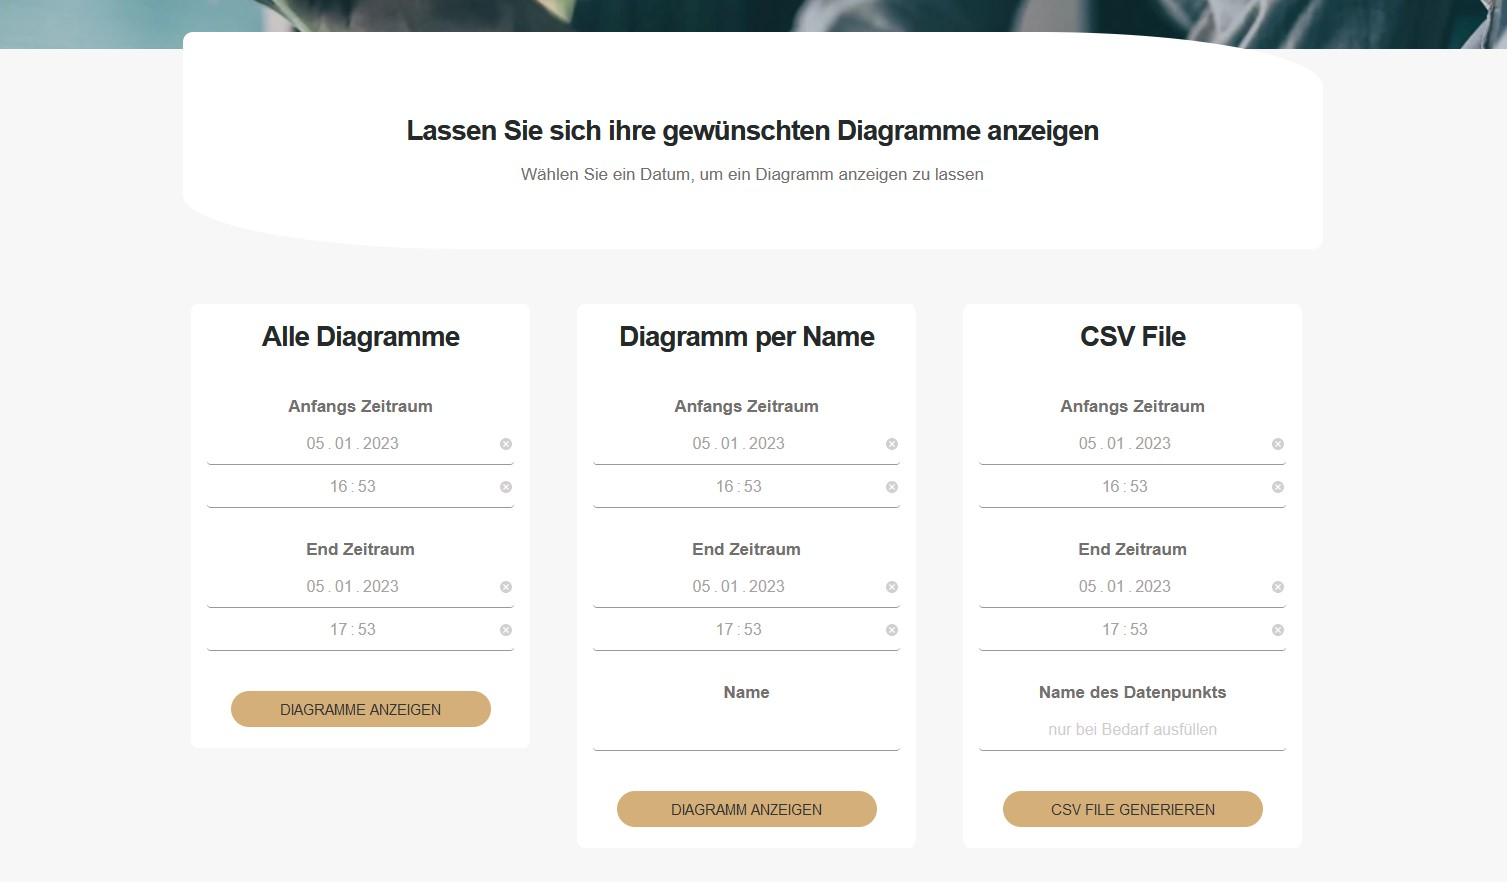
\includegraphics[scale=0.45]{pics/FlexLoggerWebsiteFormulare.jpg}
    \caption{Website Hauptseitenansicht}
    \label{fig:impl:FlexLoggerHauptseitenAnsicht}
\end{figure}

\begin{figure}
    \centering
    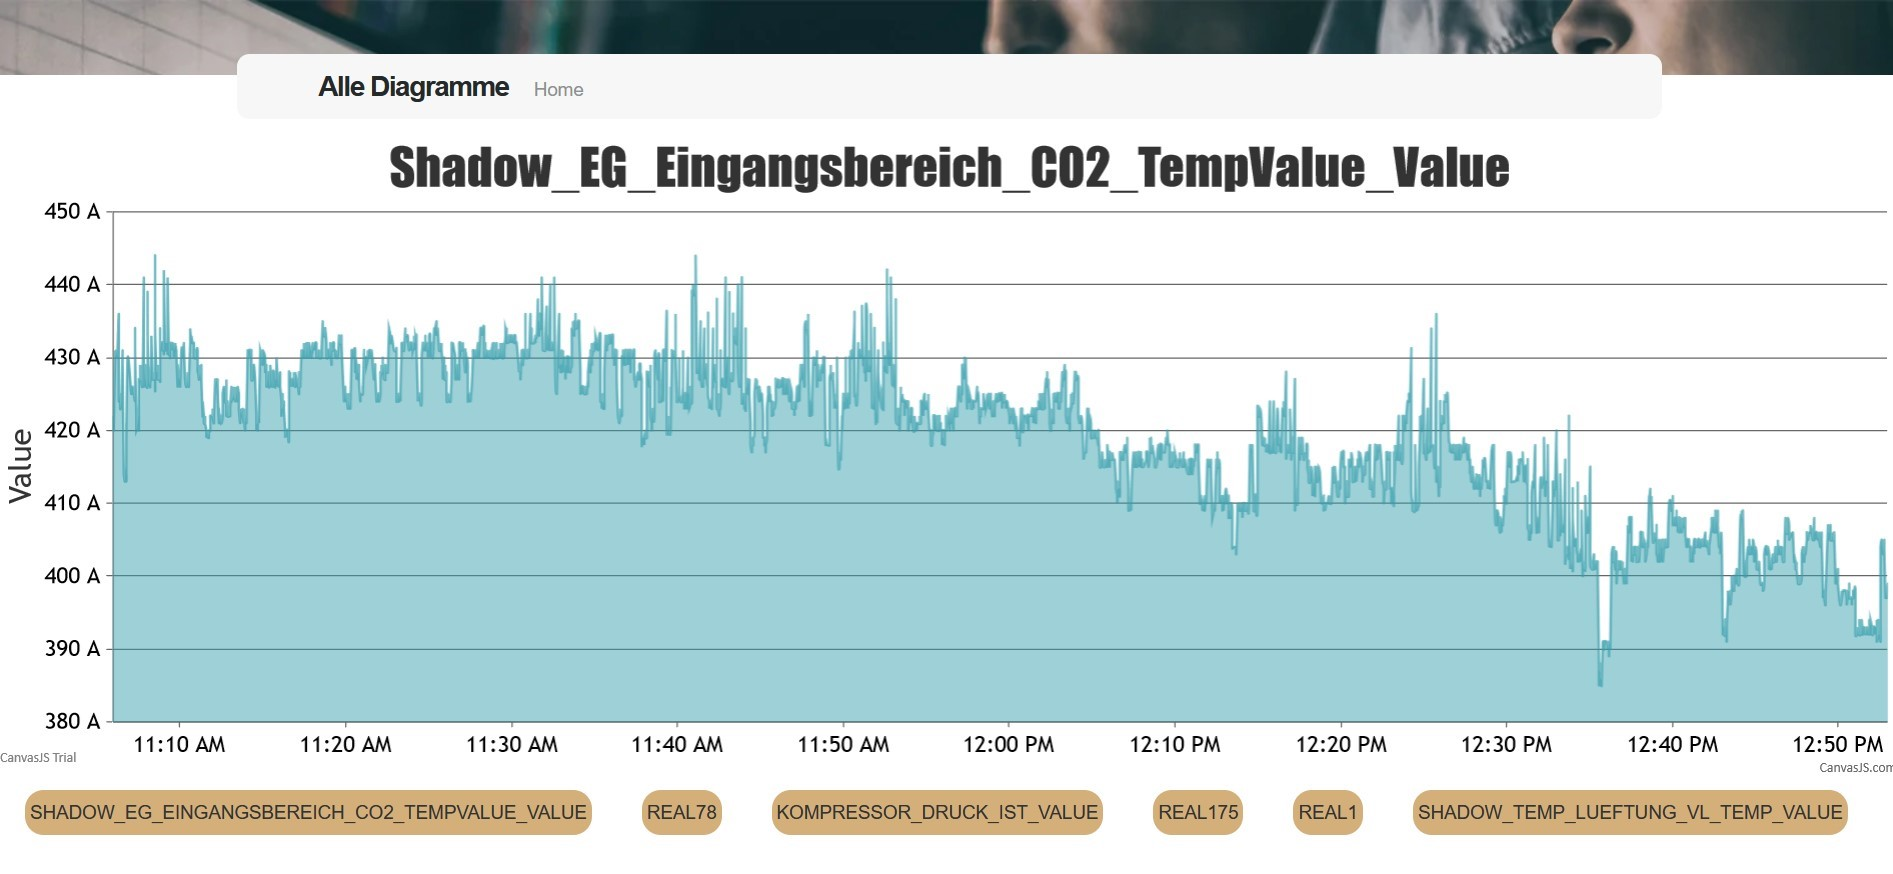
\includegraphics[scale=0.35]{pics/FlexLoggerWebsiteDiagramm.jpg}
    \caption{Website Diagrammansicht}
    \label{fig:impl:FlexLoggerDiagrammAnsicht}
\end{figure}

\subsubsection{App-Component}
In der TypeScript Klasse der App-Komponente wird ansich ein Titel definiert, dieser trägt in diesem Fall den Namen „flexloggerFE2“. Im HTML-File ist dabei ein Router-Outlet definiert. Durch dieses wird das Routing im Projekt ermöglicht. Das heißt jede Komponente wird praktisch in der App-Komponente angezeigt. In der app-routing-module Klasse werden alle Pfade des Projekts definiert. Dabei wird jeweils ein String als Pfad angeben, sowie eine Komponente definiert, zu welcher der Pfad führen soll. Zusätzlich wird bei den Modulen des Projekts ein RouterModule hinzugefügt, welches zusätzlich die Methode forRoot verwendet, in welchem die vorher definierten Routen als Parameter übergeben werden. In der app-module Klasse werden noch weitere Module hinzugefügt: 

\begin{compactitem}
    \item BrowserModule: Stellt einen Service zur Verfügung, mit welchem man eine Browser-app starten, sowie laufen lassen kann.    
    \item AppRoutingModule: Ermöglicht das Navigieren zwischen verschiedenen Komponenten.     
    \item HttpClientModule: Mithilfe dieses Moduls können Netzwerk Requests abgesetzt werden. Diese inkludieren GET, POST, PUT, PATCH und DELETE.    
    \item FormsModule: Durch dieses Modul können template-driven Forms erstellt werden.    
    \item ReactiveFormsModule: Mithilfe dieses Moduls kann ein reactiveForm verwenden. 
\end{compactitem}

\subsubsection{Home-Component}
Die ist die Haupt Komponente des Programms. In ihr werden 3 Formulare definiert, jedes davon hat eine andere Funktion. Im Konstruktor der Komponente werden verschiedenste Parameter übergeben:

\begin{compactitem}
    \item HttpService: Dies ist der Service, mithilfe dessen eine Server-Verbindung zum Backend aufgebaut werden kann.    
    \item Router: Mithilfe dieses in Angular eingebauten Features kann auf der Website zwischen den Komponenten gewechselt werden.        
    \item ActivatedRoute: Mithilfe dieses Parameters können Daten über Komponenten hinweg übergeben werden.    
    \item FormBuilder: Durch diesen Parameter können Reactive Formulare erstellt werden??
    \item ValidatorService: Wird später verwendet, um die Richtigkeit der Eingabe bei den Formularen zu garantieren.
\end{compactitem}

Im Konstruktor selbst, wird das heutige Datum sowie das heutige Datum plus einer Stunde gesetzt.
Um die Komponente zu initialisieren, wird in der ngOnInit()-Methode die initForms-Methode aufgerufen. Diese initialisiert alle 3 Formulare, indem sie die Variablen in den Formularen, sowie Validatoren setzt. Dabei werden bei den Variablen jeweils ein Standard-Wert gesetzt. Die gesetzten Validatoren überprüfen dabei, ob die Daten korrekte Eingaben in den Formularen sind. 

Weiteres findet man in der Komponente zwei Methoden, welche sich um das Routing kümmern. Diese kommen beim Klicken der Buttons der Formulare zum Einsatz, um die Komponente, welche angezeigt wird, zu wechseln. Die benötigten Daten werden dabei in der URL übergeben.

Die nachfolgende Methode ist für das Generieren sowie das Downloaden einer CSV-Datei zuständig. Zuallererst wird die checkCSV-Methode aufgerufen, in welcher überprüft wird, ob in dem ausgewählten Zeitraum Daten verfügbar sind.

Wenn die checkCSV-Variable als true gesetzt wurde, wird überprüft, ob der Namenparameter im Formular nicht leer ist. Trifft dies ein, wird mithilfe eines Timers und des Http-Service eine CSV-Datei generiert, welche alle Datenpunkte in dem richtigen Datumsbereich generiert. Nachdem das Generieren erfolgreich abgeschlossen wurde, wird der Download der Datei gestartet. Dieser Download wird mithilfe der window.open() Methode verwirklicht. Wenn der Namenparameter in dem Formular einen Namen enthält, so wird ein CSV-File generiert, welches nur die Daten eines Datenpunkts beinhält.

Wenn der Fall eintrifft, dass die checkCSV-Variable auf false gesetzt wurde, dann werden die Errors des Namenparameters auf true gesetzt. Dadurch wird unter dem Formular eine Fehlermeldung ausgegeben, um dem User eine Rückmeldung der Formulareingabe zu geben.

\subsubsection{Canvas-Chart-Component}

In dieser Komponente wird ein Diagramm erstellt, in welchem anschließend mithilfe von verschiedenen Buttons die gewünschten Daten angezeigt werden.  

Der erste wichtige Teil der Komponente ist das Erstellen der Diagramm Optionen. In diesen kann man verschiedenste Attribute eines Diagramms definieren: 

\begin{compactitem}
    \item animationEnabled: Stellt ein, ob beim ersten Anzeigen eines Diagramms jeder Punkt des Diagramms flüssig geladen wird, um ein dynamischeres Ergebnis zu erhalten.    
    \item title: Setzt den Titel fest, welcher als Überschrift über dem Diagramm stehen soll.          
    \item axisY: Legt den Titel der Y-Achse fest, diese Einstellung kann genauso auf der X-Achse getätigt werden.    
    \item data: Dies ist die wichtigste Einstellung der Diagramm Optionen. Sie legt den Typ des Diagramms fest (in diesem Fall ist es ein Liniendiagramm), die Farbe des Diagramms und setzt die Datenpunkte fest. Beim ersten Laden der Seite werden die Datenpunkte der X- und Y- Achse auf 0 bzw. den 01.01.1970 gesetzt. 
\end{compactitem}

Beim Laden der Seite wird zuerst im Konstruktor der Komponente eine Funktion namens onload() ausgeführt. Diese ist dafür zuständig, die erforderlichen Daten mithilfe des http-Service aus dem Backend zu bekommen. Zuerst werden hierfür die übergebenen Werte aus dem Formular mithilfe von Route Snapshots übergeben. Anschließend wird durch den http-Service eine getLogEntries-Methode aufgerufen, diese gibt die Werte zurück, welche das erforderliche Datum besitzen. Diese werden nun in einem Array gespeichert, um weiter verwendet zu werden.

Ion der nächsten Zeile des Konstruktors befindet sich ein Timer, welcher nach 1? Sekunde den darauffolgenden Code durchführt. In diesem Code wird zuallererst eine getFiles-Methode ausgeführt, diese gibt das vorher erstellte Array zurück. Das IF-Statement eine Zeile darunter garantiert, dass die Länge des Arrays nicht 0 beträgt, ansonsten wird die Fehlermeldung "Zu Ihrem ausgewählten Zeitpunkt wurden keine Daten gefunden." ausgegeben. Bei einem positiven Ergebnis des IF-Statements werden nachfolgend vier Methoden aufgerufen: 

\begin{compactitem}
    \item getListOfDatapointNames(): Diese Methode kümmert sich darum, eine Liste der Namen für die Buttons zu erstellen. Diese Buttons sind später dafür zuständig, zwischen den angezeigten Daten zu wechseln. 
    Um zu verhindern, dass der Name eines Datenpunkts öfters in der Liste vorkommt, wird am Beginn eine Boolean-Variable namens nameInList erstellt. Diese wird vorerst auf False gesetzt.
    Anschließend wird ein vorher initialisiertes Array auf ein leeres Array gesetzt, in welches danach die Namen hinzugefügt werden. Um alle Namen aus den Daten zu erlangen, wird eine for-Schleife verwendet, welche alle vorher erhaltenen Daten durchgeht. Der erste Name wird immer hinzugefügt, daher wenn die Länge des leeren Arrays 0 ist, wird der erste name hinzugefügt. Sonst wird eine weitere for-Schleife betreten, welche alle Elemente der List der Namen durchgeht. Wenn ein Element bereits vorhanden ist, wird die nameInList Variable auf true gesetzt. Später wird in einem weiteren If-Statement überprüft, ob diese Variable auf True oder False gesetzt ist. Bei einem False wird dabei der Name in die Liste hinzugefügt. Durch dieses Verfahren wird sichergestellt, dass kein Name doppelt in der Liste vorkommt und somit Buttons nicht doppelt angezeigt werden.    
    \item changeData()
    Hier werden die geänderten Daten in die Diagramm Optionen gespeichert. Um dies umzusetzen, wird als Parameter ein String namens filterString übergeben. Mithilfe diesem und einer For-Schleife werden alle Datenpunkte herausgefiltert, welche nicht den gewünschten Namen besitzen. Die richtigen Daten werden nun im Array dynamicLogLines gespeichert. Nach dem Aussortieren der Daten wird mit einem IF-Statement überprüft, ob die erste Stelle des dynamicLogLines nicht undefiniert ist. Wenn dies der Fall ist, wird der erste Datenpunkt, sowie der Titel in den Diagramm Optionen gesetzt. Danach werden die restlichen Datenpunkte mithilfe einer For-Schleife in den Diagramm Optionen gespeichert.               
    \item setChartOptions()
    Beim Aufrufen dieser Methode werden die Diagramm Optionen neu gesetzt. In diesem Fall wird der Titel, die Einheit und die Datenpunkte des Diagramms erneuert.        
\end{compactitem}

Anschließend wird eine Boolean-Variable namens showChart auf True gesetzt, wenn dieser Fall eintritt, wird auf der Website ein Diagramm angezeigt. 

\subsubsection{Canvas-Chart-Single-Component}
Die Komponente ist vom Aufbau her sehr ähnlich wie die Canvas-Chart-Komponente. Genau wie in der anderen Komponente werden zuerst einige Methoden im Konstruktor aufgerufen. Der größte Unterschied dabei ist, dass keine Buttonnamen erstellt werden, bzw. auch keine Buttons angezeigt werden. 

\subsubsection{HttpService}
Der Service ist dafür zuständig, die jeweiligen Daten aus dem Backend zu beschaffen. Zuerst wird ein String definiert in welchem die URL des Backend gespeichert ist. Im Konstruktor wird der sogenannte HttpClient als Parameter übergeben, er ist der Hauptakteur in der Klasse. Mithilfe von ihm kann eine Verbindung zum Server hergestellt werden. 

In dem Service befinden sich mehrere Methoden. Allgemein kann man sagen, dass man mit dem HttpClient jeweils einen GET-Request absetzt, welcher jeweils ein anderes Ergebnis liefert, je nachdem welche URL man als Parameter übergibt.

Die ersten beiden haben jeweils als Rückgabe-Paramater ein LogEntry Array. Beide geben die gesuchten Daten in einem bestimmten Zeitraum zurück, lediglich kann man bei der zweiten Methode noch einen Namen hinzufügen. Die Daten, welche die Zeiträume definieren, werden als Parameter in den Methoden übergeben. Die nächsten Methoden sind allesamt für das Downloaden eines CSV-Files verantwortlich. Dabei kümmern sich die ersten beiden um das Erstellen der CSV-Datei, die dritte ist für den eigentlichen Download verantwortlich. Um die CSV-Datei zu erstellen, werden wiederum die gewünschten Daten übergeben und anschließend wird daraus eine URL gebaut und ein GET-Request abgesetzt. Der einzige Unterschied zwischen den Methoden ist abermals ein zusätzlicher Name-Parameter. Die downloadCSV-Methode verwendet wie die anderen Methoden einen GET-Request, allerdings hat sie den weiteren Parameter responseType. Dieser ist notwendig, da innerhalb des Requests eine CSV-Datei gedownloadet wird und somit der Response-Type Array-Buffer definiert werden muss. 

\subsubsection{ValidatorService}
Der ValidatorService ist dafür zuständig, die Richtigkeit der Eingabe im Formular zu überprüfen. Wenn diese als nicht akzeptabel erkannt wurden, werden die Errors der Parameter auf true gesetzt, und somit eine Fehlermeldung ausgegeben.

Die match-Methode überprüft ob jedes eingegebene Datum als valide Eingabe akzeptiert werden kann. Dabei werden zuerst alle Controls des Formulars übergeben. Bei der ersten Überprüfung handelt es sich darum, ob das Startdatum hinter dem Enddatum liegt. Bei Bestätigung dieser Überprüfung werden die Errors mit dem Namen dateMustBeBigger aktiviert. Anschließend wird der Fall überprüft, wenn die beiden Daten gleich sind, die Zeiten sich allerdings unterscheiden, d.h. der Zeitraum am gleichen Tag stattfindet. Dies ist grundsätzlich erlaubt allerdings nur, wenn die Startzeit kleiner ist als die Endzeit. Wenn dies nicht der Fall ist, wird der Error timeMustBeBigger aktiviert.

\subsubsection{LogEntry Model}
Hier wird ein Model erstellt, welches den Namen LogEntry trägt, in diesem werden die Parameter dpId, value, unit und timeStamp definiert. Das Model wird dazu verwendet, um die vorher geloggten Daten aus der Datenbank weiterzuverwenden. 

\subsection{CanvasJS}
Mithilfe von CanvasJS, welche eine HTML5 und Javascript Charting library ist, wird das Anzeigen der Daten in Diagrammen ermöglicht. 

\begin{spacing}{1}
    \section{Logging}\label{section:logging}
    \end{spacing}

% < 1 Big Data in der Praxis - Lösungen mit Hadoop, Spark, HBase und Hive. Daten speichern, aufbereiten, visualisieren. 2. erweiterte Auflage, von  Jonas Freiknecht, Stefan Papp, 2018, S
% < 1 https://www.omega.com/en-us/resources/data-loggers
% 0 https://www.researchgate.net/profile/Anne-Ojala/publication/254255682_Eddy_Covariance_A_Practical_Guide_to_Measurement_and_Data_Analysis/links/00b7d51fbaa83999a4000000/Eddy-Covariance-A-Practical-Guide-to-Measurement-and-Data-Analysis.pdf#page=80
Data Logging kann dazu verwendet werden, Code zu debuggen oder große Datenmengen zu speichern, um diese später auszuwerten. Im Allgemeinen ist ein Datalogger ein Instrument, welches Veränderungen unter bestimmten Bedingungen während einer gewissen Zeitspanne aufzeichnet. Ein Datenlogger verwendet häufig Sensoren, um Daten zu sammeln. Anschließend können die Daten ausgelesen, visuell dargestellt und/oder ausgewertet werden. Die Daten, welche von Datenloggern ausgelesen werden, sind meist Druck, Temperatur, Luftfeuchtigkeit, Spannung oder Stromstärke. \cite{DataLogging} 

Die gespeicherten (geloggten) Daten können zum Beispiel dazu verwendet werden, 

\begin{compactitem}
    \item um die Temperatur und die Luftfeuchtigkeit in einem Gebäude zu überprüfen
    \item Information zur Gebäudewartung zur Verfügung zu stellen, dies betrifft das Heizen, die Belüftung, wie die Klimatisierung. Diese ständige Überprüfung der Daten kann den Energieverbrauch reduzieren
    \item die Wachs-Bedingungen von Pflanzen in der Landwirtschaft zu beobachten
    \item die Impfstoff-Lagerung in medizinischen Einrichtungen zu überwachen
    \item die Temperatur von Lebensmittel zu überprüfen
\end{compactitem}
\cite{DataLogging}

Logging bieten eine große Flexibilität und eignet sich gut, um große Datenmengen zu erfassen und auszuwerten. \cite{BigDataBuch}

\subsection{Loggen der Daten in der Firma}
Um die Daten zu loggen, also abzuspeichern, werden diese aus sogenannten Datenpunkten aus der firmentinternen FlexCloud ausgelesen. Diese werden angesprochen und aus ihnen kann dann der aktuelle Wert des Datenpunkts ausgelesen werden, siehe \ref{fig:impl:datenlogging}.
Beispiele für Datenpunkte der Firma FlexSolution, die ausgelesen werden: 

\begin{compactitem}
    \item Daten der Ladestationen
    \item Daten der Photovoltaik-Anlage am Dach
    \item die Temperatur in den Firmengebäuden
    \item Kompressor-Druck von Maschinen
    \item weitere Maschinendaten
\end{compactitem}

\begin{figure}[h t]
    \centering
    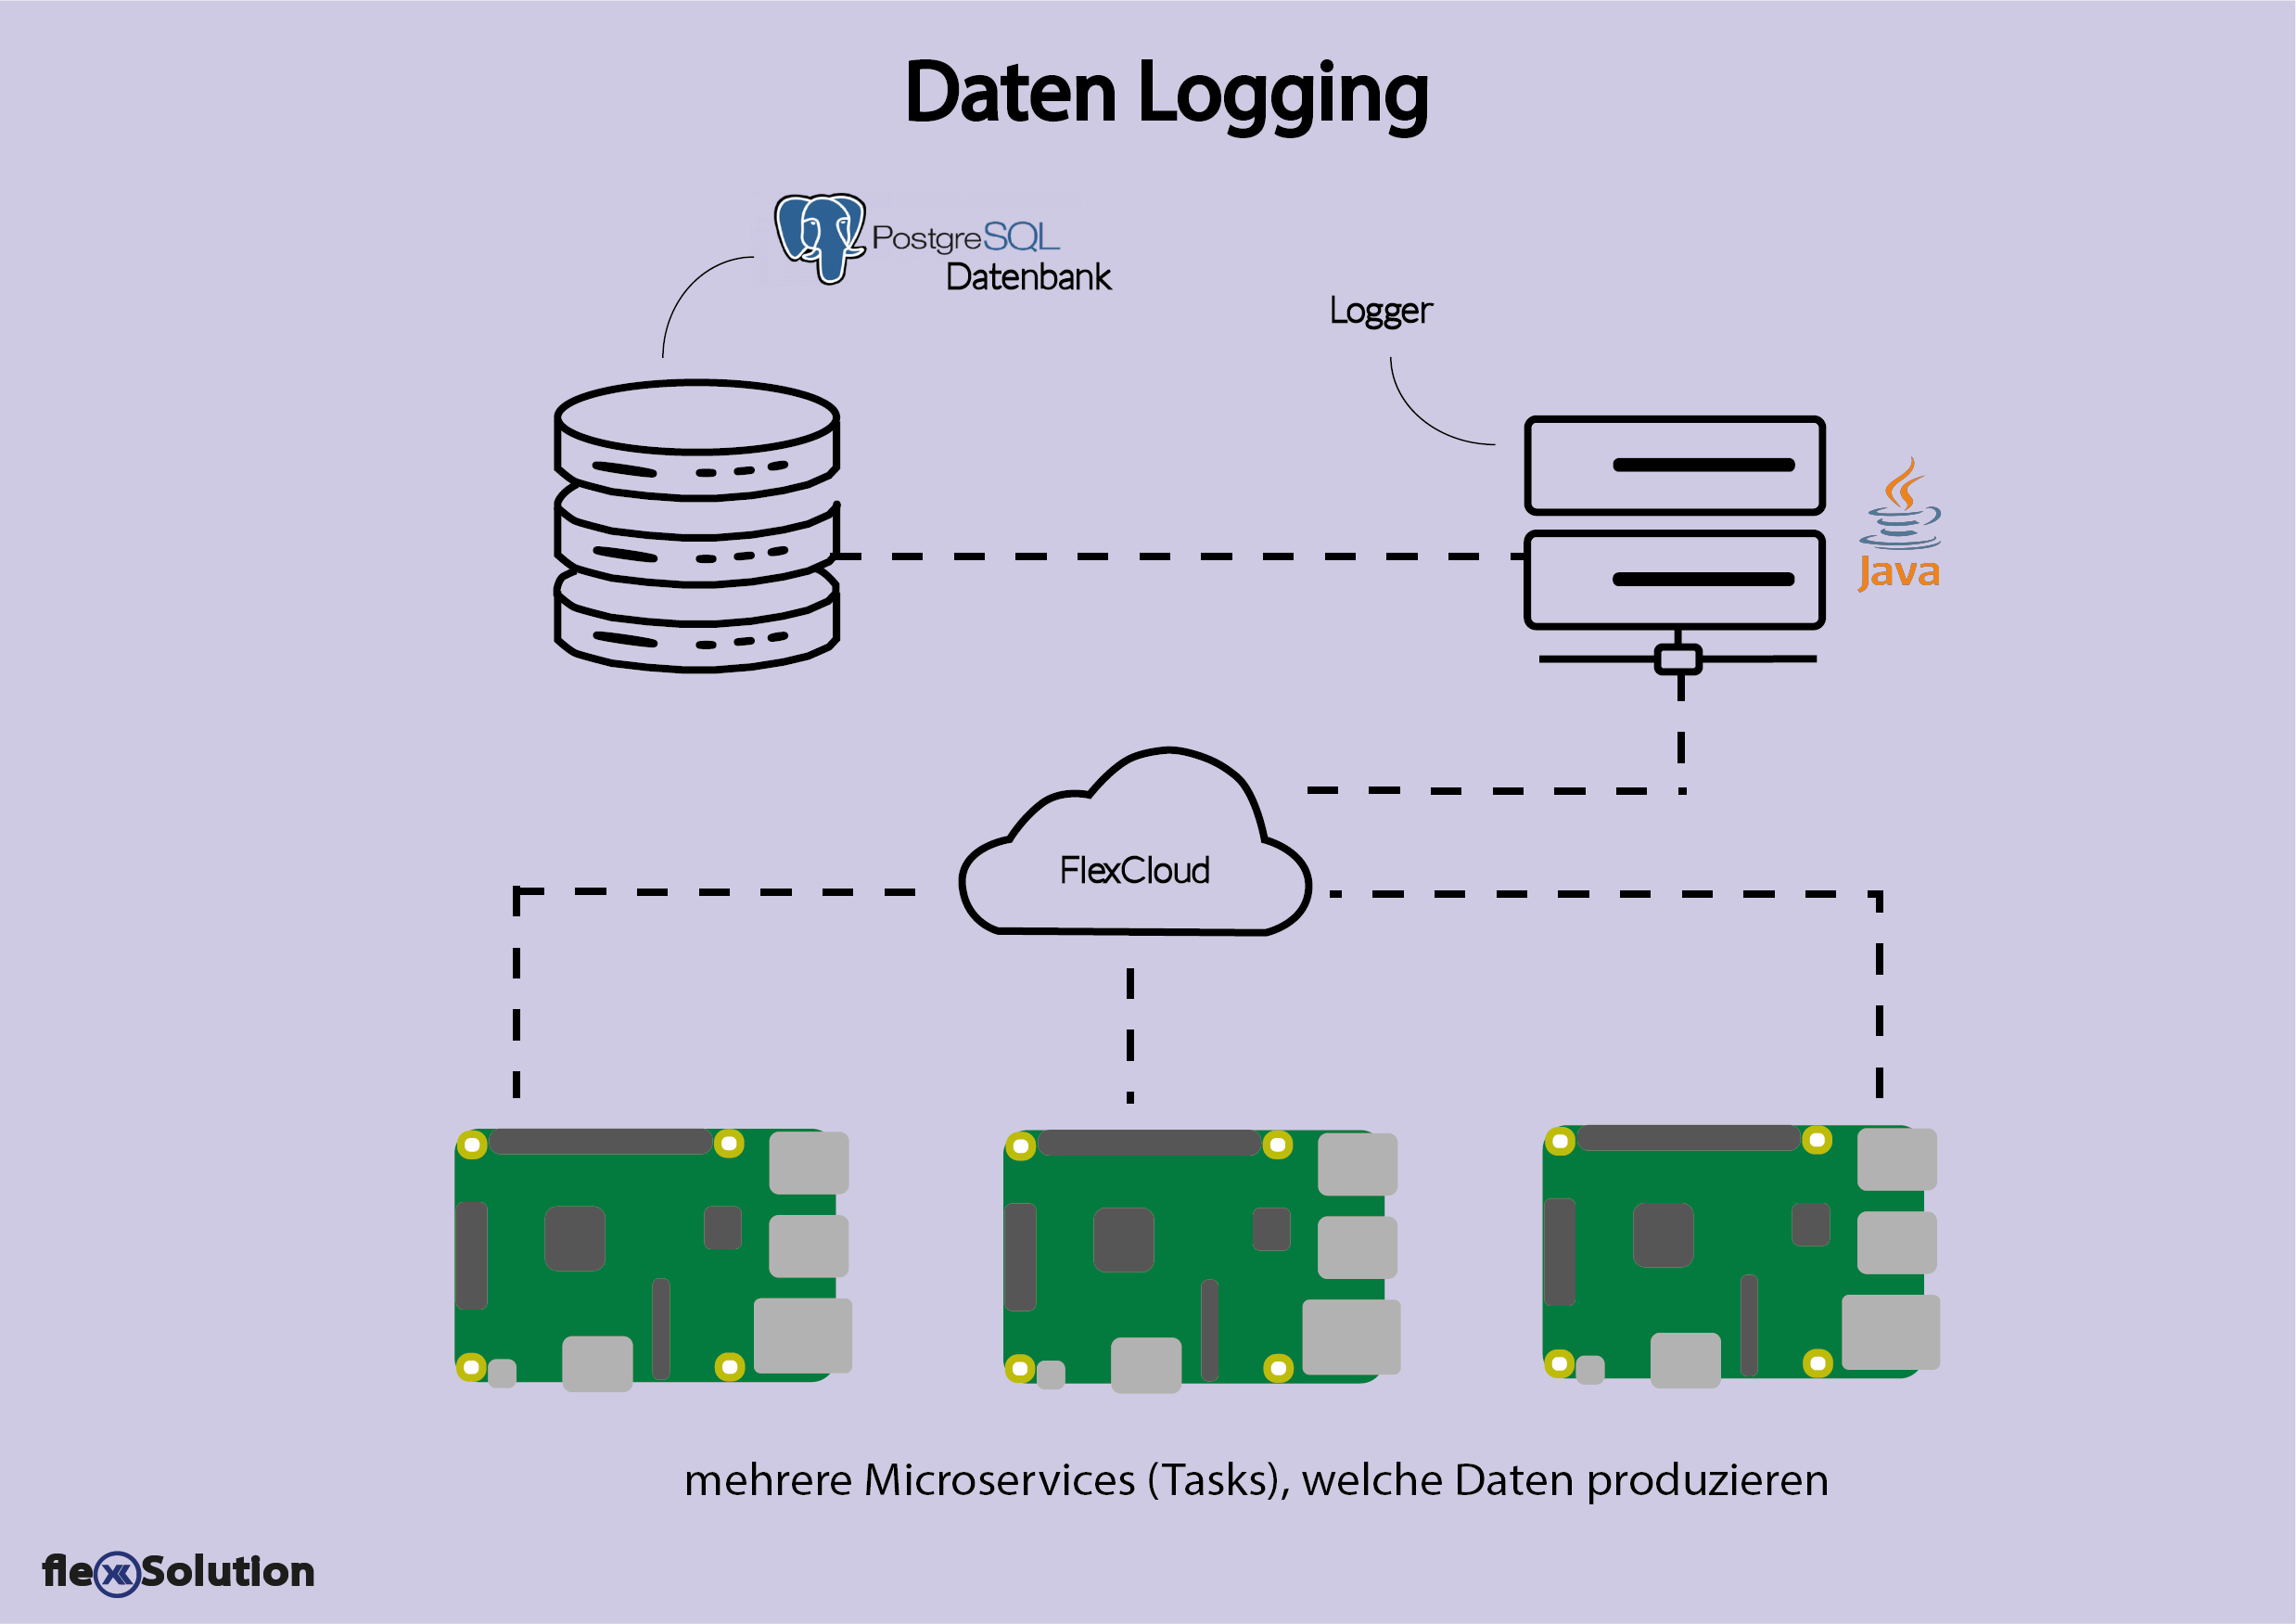
\includegraphics[scale=0.7]{pics/datenlogging.png}
    \caption{Daten Logging}
    \label{fig:impl:datenlogging}
\end{figure}

Das Logging-Programm wird mithilfe des Terminals gestartet. Sobald dieses gestartet wurde, siehe \ref{fig:impl:loggerStart}, werden kontinuierlich Daten in die Datenbank gespeichert. Dies kann in der Ausgabe des Loggers beobachtet werden, siehe \ref{fig:impl:loggerLog}. Um den Logger anschließend zu stoppen, wird ein ähnlicher Command wie beim Starten verwendet, siehe \ref{fig:impl:loggerEnd}.

\begin{figure}[h t]
    \centering
    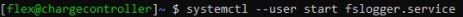
\includegraphics[scale=1.3]{pics/loggerStart.JPG}
    \caption{Logger Programm wird gestartet}
    \label{fig:impl:loggerStart}
\end{figure}

\begin{figure}[h t]
    \centering
    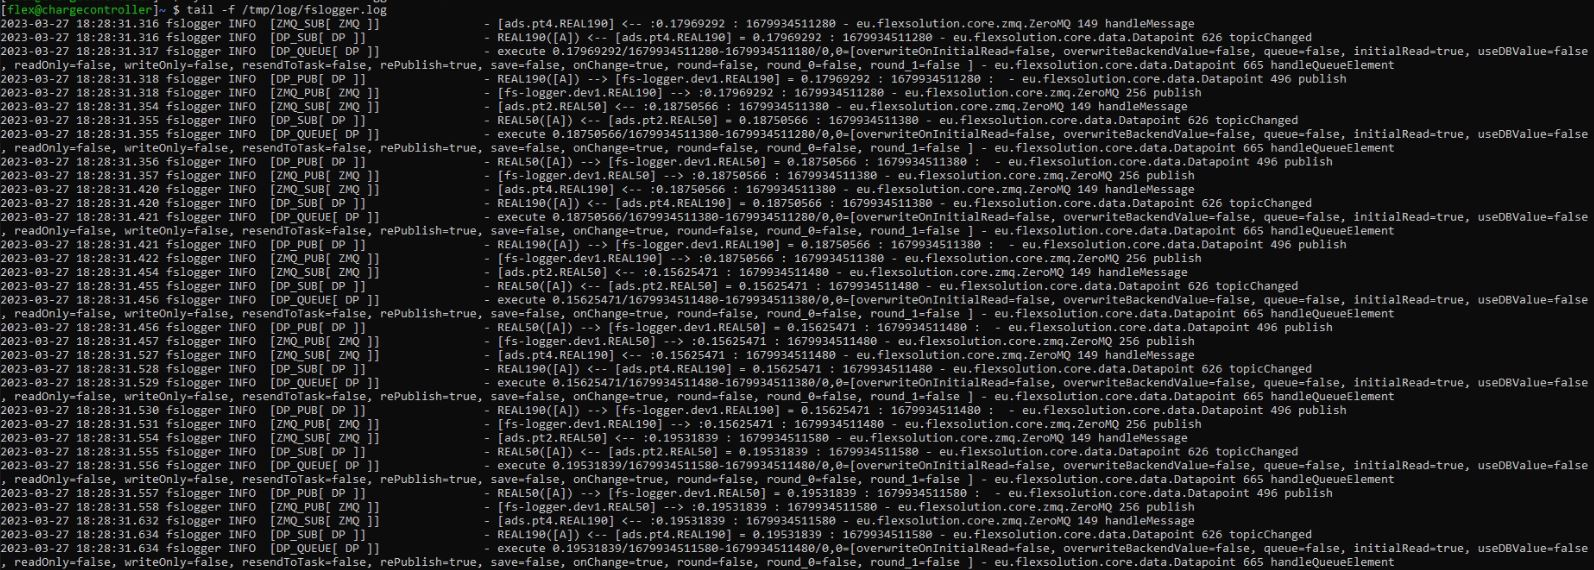
\includegraphics[scale=0.4]{pics/loggerLog.JPG}
    \caption{Ausgabe des Logger Programms}
    \label{fig:impl:loggerLog}
\end{figure}

\begin{figure}[h t]
    \centering
    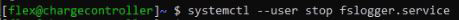
\includegraphics[scale=0.75]{pics/loggerEnd2.JPG}
    \caption{Logger Programm wird gestoppt}
    \label{fig:impl:loggerEnd}
\end{figure}

\subsection{Log4J}
% < 1 https://books.google.at/books?hl=de&lr=&id=hZBimlxiyAcC&oi=fnd&pg=PA9&dq=log4j&ots=QiOna081Z6&sig=9h3lwPqN-rm07kAHln-tLSUfgJY&redir_esc=y#v=onepage&q=log4j&f=false The Complete Log4j Manual, von: Ceki Gülcü S15
% < 1 https://logging.apache.org/log4j/2.x/
Log4J ist ein Framework, um Anwendungsmeldungen von Java zu loggen.
Das Design von Log4J konzentriert sich vor allem darauf, schnell, flexibel und leicht verständlich zu sein. Da Logging eine Applikation verlangsamen kann, wird vor allem ein Wert auf die Schnelligkeit gelegt. \cite{log4JBuch} 

Es ist ein populäres Logging-Package für Java. Logging liefert präzise Informationen über den Ablauf einer Applikation. \cite{log4J}


Anwendungen, welche Log4j verwenden, fordern vom LogManager einen Logger mit einem bestimmten Namen an. Der LogManager sucht den entsprechenden LoggerContext und ruft dann dessen Logger ab. 
Wenn erst ein Logger erstellt werden muss, wird er mit der LoggerConfig verknüpft, die entweder 

\begin{compactitem}
    \item[a)] den gleichen Namen wie der Logger, 
    \item[b)] den Namen eines übergeordneten Pakets oder 
    \item[c)] die Stamm-LoggerConfig enthält.
\end{compactitem}

LoggerConfig-Objekte werden aus Logger-Deklarationen in der Konfiguration erstellt. Die LoggerConfig ist mit den Appendern verbunden, welche die LogEvents tatsächlich liefern, siehe Abb. \ref{fig:impl:log4jArchitektur}. \cite{log4J}

\begin{figure}[h t]
    \centering
    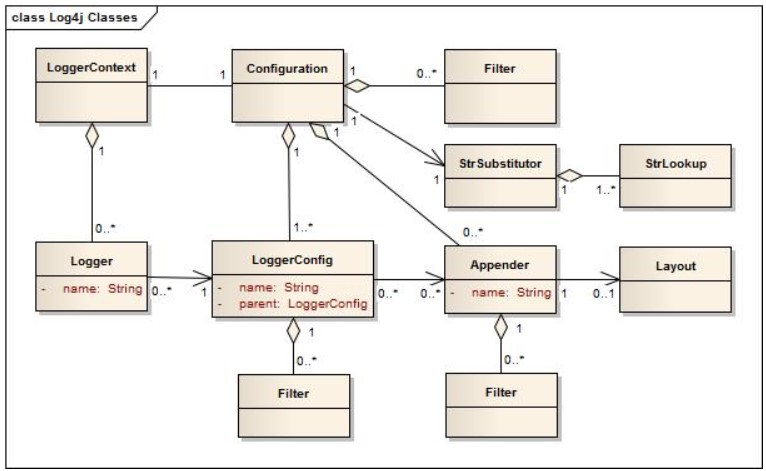
\includegraphics[scale=0.7]{pics/log4jArchitektur.jpg}
    \caption{log4J Architektur \cite{log4J}}
    \label{fig:impl:log4jArchitektur}
\end{figure}

\begin{spacing}{1}
    \section{Threads}\label{section:threads}
    \end{spacing}
 
% \subsection{Streams}
 
% \subsection{Lambda}
 
\subsection{Serialisierung (Nebenläufigkeit und Parallelität)}
% 1 Java ist auch eine Insel - Einführung, Ausbildung, Praxis ; von: Christian Ullenboom
Wenn in Java über Nebenläufigkeit gesprochen wird, sind dabei Threads gemeint. Diese sorgen für eine gleichzeitige Abarbeitung von Programmen bzw. der Ressourcen. Dies kann umgesetzt werden, indem die Hardware mehrere Prozessoren oder Kerne besitzt und diese parallel Prozesse abarbeiten können.
 
Bei einem modernen Ein-Prozessor-Betriebssystem wirkt es oft, als wären die Prozesse parallel, doch dies wird einem nur vorgespielt, indem der Prozessor alle paar Sekunden auf einen anderen Prozess wechselt. Bei einem Betriebssystem mit mehreren Kernen, werden die Prozesse wirklich parallel bearbeitet.
 
\subsubsection{Nebenläufigkeit von Programmen steigert Geschwindigkeit}
Wie nebenläufige Abarbeitung die Performance bei einem Einprozessorsystem beschleunigt, kann an folgendem Beispiel-Programm betrachtet werden:
 
\begin{compactitem}
    \item Programm führt eine Reihe von Befehlen aus
    \item Programm soll Datenbank-Report erstellen/visualisieren    
    \item Dabei können einige Prozesse nebenläufig abgearbeitet werden
    \item Diese Prozesse sind zum Beispiel: Öffnen der Datenbank, Lesen neuer Datensätze gleichzeitig mit dem Analysieren alter Daten, alte Daten können in eine Report-Datei geschrieben werden während neue Daten analysiert werden
    \item Wenn diese Prozesse parallel ausgeführt werden, kann sehr viel Zeit eingespart werden beziehungsweise die Performance sehr erhöht werden.
    \item Dieses Beispiel zeigt allerdings auch, dass Nebenläufigkeit sehr gut geplant werden muss.
\end{compactitem}
 
 
\subsection{Concurrency/Gleichzeitigkeit}
% 0 https://www.baeldung.com/java-util-concurrent
% 0 https://reader.elsevier.com/reader/sd/pii/S0167642305000663?token=33C353917B1806AF8A5D40D069D18442FDCF27727ADE08478255219D5D7D6849BA4E8FAE2A474A3FDCD3CC0A36740643&originRegion=eu-west-1&originCreation=20230105151331
% 1 Java ist auch eine Insel - Einführung, Ausbildung, Praxis; von: Christian Ullenboom
Die Ausführung des Programmcodes wird bei einem modernen Betriebssystem von Prozessen, welche jeweils mindestens einen Thread beherbergen, ausgeführt. Das Interessante daran ist, dass nicht etwa die Prozesse nebenläufig ausgeführt werden, sondern die Threads. Dabei können die Threads auf den gleichen Adressraum zugreifen.
 
\subsubsection{Zustände eines Threads}
\begin{compactitem}
    \item Noch nicht erzeugt: Lebenslauf beginnt mit Schlüsselwort \texttt{new}
    \item Running (Laufend) und Not Running (Nicht laufend); Thread kommt in den Zustand Running, wenn die Methode \texttt{run()} aufgerufen wird. Wenn ein anderer Thread den Prozessor des aktuellen Threads übernimmt, kommt der Thread in den Zustand Not Running.    
    \item Waiting (Wartend): Thread befindet sich in einem Wartezustand
    \item Beendet: Aktivität des Threads wurde beendet
\end{compactitem}
 
\subsection{Aufbau eines Threads}
\subsubsection{Interface Runnable}
Dem Thread muss ein Befehlsobjekt des Typs Runnable übergeben werden \ref{lst:impl:javaRunnable}, um wissen zu können, welcher Code ausgeführt werden soll.
Wenn der Thread gestartet wird, werden die Codezeilen im Befehlsobjekt nebenläufig zum anderen Code in dem Programm ab.
 
\begin{lstlisting}[language=java,caption=Java Runnable,label=lst:impl:javaRunnable]
    interface java.lang.Runnable
\end{lstlisting}
 
Durch dieses Interface kann nun die run()-Methode verwendet werden. \ref{lst:impl:threadExample}
 
\begin{lstlisting}[language=java,caption=Einfaches Thread Beispiel,label=lst:impl:threadExample]
    public class CommandThread implements Runnable { 
        @Override public void run() {   
            ...
            }
        }
\end{lstlisting}
 
Dieser Thread kann nun in einer anderen Klasse verwendet werden, indem er zum Beispiel gestartet (\texttt{thread.start()}) oder gestoppt (\texttt{thread.stop()}) wird. \ref{lst:impl:threadStart}
 
\begin{lstlisting}[language=java,caption=Thread erstellen/starten,label=lst:impl:threadStart]
    Thread t1 = new Thread( new CommandThread() );
    t1.start();
\end{lstlisting}
 
Zusätzlich ist es auch noch möglich, den Thread mit (\texttt{thread.sleep(ms)}) zu pausieren.
 
\subsection{BlockingQueue}
% 1 https://jenkov.com/tutorials/java-util-concurrent/blockingqueue.html#java-blockingqueue-tutorial-video
% 0 https://dl.acm.org/doi/pdf/10.1145/3472456.3472458
% 0 blocking queue:  https://books.google.at/books?id=mvzgNSmHEUAC&pg=PT856&dq=java+blocking+queue&hl=de&sa=X&ved=2ahUKEwiF4Jej3bD8AhUNxwIHHcjWBlMQ6AF6BAgEEAI#v=onepage&q=java%20blocking%20queue&f=false
 
Eine BlockingQueue hat typischerweise einen Thread, welcher Objekte produziert und einen anderen, welcher die Objekte konsumiert. \ref{fig:impl:BlockingQueue}
 
\begin{figure}[h t]
    \centering
    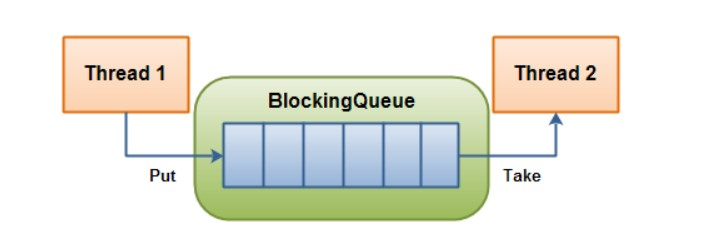
\includegraphics[scale=0.5]{pics/blockingQueue.jpg}
    \caption{Blocking Queue}
    \label{fig:impl:BlockingQueue}
\end{figure}
 
Der produzierende Thread wird weiterhin Objekte produzieren und sie zur BlockingQueue hinzufügen, bis das Limit der Queue erreicht wird. Wenn dieses Limit erreicht wird, wird der Producer-Thread blockiert, während er versucht ein neues Objekt hinzuzufügen. Der Producer Thread bleibt dabei blockiert, bis ein Consumer Thread ein Objekt aus der Queue nimmt.
 
Auf der anderen Seite nimmt der Consumer Thread Objekte aus der Queue, um sie weiter zu verarbeiten. Wenn der Thread versucht ein Objekt aus einer leeren Queue zu nehmen, wird er blockiert, bis der Producer-Thread ein Objekt in die Queue hinzufügt.
 
\subsubsection{BlockingQueue Methoden}
Um die Blocking Queue mit Daten zu bespielen, gibt es spezielle Methoden.
 
\begin{center}
    \begin{tabular}{ |c|c| }
     \hline
     put(o) & fügt Objekte in die BlockingQueue hinzu \\
     \hline
     take() & nimmt Objekte aus der BlockingQueue \\
     \hline
    \end{tabular}
    \end{center}
 
Wenn die Operation bei einer der Methoden erfolglos war, blockiert die Methode, bis die Operation erfolgreich war.
 
\subsubsection{Java Blocking Queue Beispiel}
Das Beispiel unten angeführt verwendet eine ArrayBlockingQueue als Implementation.
 
 
 
\begin{lstlisting}[language=java,caption=Java BlockingQueue Beispiel,label=lst:impl:blockingQueue]
    public class BlockingQueueClass {
    public static void main(String[] args) throws Exception {
        BlockingQueue blockingQueue = new ArrayBlockingQueue(2048);
        Producer producer = new Producer(queue);
        Consumer consumer = new Consumer(queue);
        new Thread(producer).start();
        new Thread(consumer).start();
        Thread.sleep(4000);
    }
    #################################################
 
    public class Producer implements Runnable{
        protected BlockingQueue queue = null;
        public Producer(BlockingQueue queue) {
            this.queue = queue;
        }
        public void run() {
            try {
                queue.put("object1");
                Thread.sleep(1000);
                queue.put("2");
            } catch (InterruptedException e) { e.printStackTrace();}
    }}
    #################################################
    public class Consumer implements Runnable{
        protected BlockingQueue queue = null;
        public Consumer(BlockingQueue queue) {
            this.queue = queue;
        }
        public void run() {
            try {
                System.out.println(queue.take());
                System.out.println(queue.take());
            } catch (InterruptedException e) { e.printStackTrace();}
    }}
}
\end{lstlisting}
 
\subsection{Service executer}
% 0 https://www.baeldung.com/java-executor-service-tutorial
% 1 Java ist auch eine Insel - Einführung, Ausbildung, Praxis; von: Christian Ullenboom
Der Service Executer hilft dabei, den eigentlichen arbeitenden Thread von dem Runnable zu trennen. Denn, wenn ein Thread erzeugt wird, muss das Runnable-Objekt im Konstruktor übergeben werden, dies kann zu Problemen führen, da das Thread-Objekt somit nicht vorher erstellt bzw. aufgebaut werden kann. Ein weiterer Grund, das Runnable und den Thread zu teilen, ist, dass ein Thread nicht einfach so ein anderes Runnable bearbeiten kann, da dieses vorher schon zugewiesen wurde.
 
% \subsection{Java Futures}
% 0 https://www.baeldung.com/java-future
% \subsection{Java Completablefutures}
 
 
% \subsection{First come first serve (Möglichkeiten Prozesse abzuarbeiten)}
 


% \begin{spacing}{1}
%    \section{Performance}\label{section:performance}
%    \end{spacing}
%% https://www.usenix.org/legacy/publications/library/proceedings/neworl/full_papers/seltzer.pdf
% https://cs.brown.edu/courses/cs227/archives/2008/Papers/Compression/GraefeShapiro.pdf
\subsection{Grenzen (Wie viel Daten gleichzeitig kommen können)}
\subsection{Bandbreite}
\subsection{Menge der Datenpunkte}

\begin{spacing}{1}
    \section{Abspeicherung von Daten}\label{section:savedata}
    \end{spacing}
\subsection{Vergleich Vor- und Nachteile JSON vs CSV vs Datenbank}
% 0 https://www.naukri.com/learning/articles/csv-vs-json-for-your-data-science-projects/
% 1 https://www.analyticsinsight.net/csv-or-json-which-format-is-better-for-your-ai-training-data/
Vor allem wenn es darum geht, große Datenmengen abzuspeichern, ist es besonders wichtig, das richtige Datenformat auszuwählen. In diesem Abschnitt wird das CSV, das JSON, und eine herkömmliche Datenbank verglichen. 

Daten können intern oder extern generiert werden und dabei gibt es verschiedene Möglichkeiten, die Daten passend abzuspeichern. Es ist sehr wichtig, das richtige Format auszuwählen, da davon einige Faktoren abhängen. Dazu gehören die Verarbeitungsgeschwindigkeit, sowie die Speichergröße. 
Außerdem kann das Format die Skalierbarkeit, die Kompatibilität, die Cloud-Speicherkosten und die Performance-Geschwindigkeit beeinflussen. 
Konkrete Beispiele, warum bestimmte Dateiformate ausgewählt werden sollten, sind: Geld zu sparen, indem zu einem CSV-Dateiformat gewechselt wird, wenn große Datensets im Cloud-Speicher verarbeitet werden. JSON ist eine bessere Wahl, wenn es darum geht, kleinere Datensets mit einer komplexen Hierarchie zu speichern. 
Im Allgemeinen bedeutet dies, dass das richtige Datenformat Geld und Zeit spart.  

\begin{center}
    \begin{tabular}{ |c|c|c|c| } 
     \hline
     \multicolumn{4}{|c|}{Ein genauerer Vergleich (exaktere Daten kommen noch) } \\
     \hline
     \hline
     Features & CSV & JSON & Datenbank \\ 
     \hline 
     \hline
     Speicheranforderung & weniger Platz & mehr Platz & ? \\ 
     \hline
     Verarbeitungsgeschwindigkeit & schnell & langsam & ? \\ 
     \hline
     Security & sicherer & unsicherer & sicherer \\ 
     \hline
     Große oder komplexe Datensets & große Datensets & komplexe Datensets & Beides \\ 
     \hline
    \end{tabular}
    \end{center}

\subsection{CSV}
CSV ist ein Text-Dateiformat, mit der Besonderheit, dass die Werte durch Semikolons unterteilt werden. Dadurch eignet es sich sehr gut für eine Speicherung von sehr vielen Daten. Jede Reihe der CSV-Datei repräsentiert dabei eine Zeile von Daten, die Spalten werden dabei von den Strichpunkten unterteilt. Das CSV-Format kann die Nutzung von Speicherplatz, sowie das Austauschen von Daten maximieren. Strukturierte CSV-Files können außerdem einen Header enthalten, welcher jede Spalte einordnet. CSV-Dateien können außerdem nicht nur durch Semikolons, sondern auch durch Kommas, Tabs und Abstände unterteilt werden. CSV wird am meisten in Entwicklungseinrichtungen und technischen Konsumenten-Anwendungen verwendet. Ein weiterer Vorteil von dem CSV-Dateiformat ist, dass es von der meisten Datenverarbeitungs-Software importiert, konvertiert und exportiert werden kann. Mithilfe dieser Softwares kann die CSV-Dateien auch sehr einfach serialisiert oder deserialisiert werden. CSV ist ein sehr einfach aufgebautes Format und kann somit von fast jedem Datenanalysator ausgewertet werden. Als Nachteile von CSV kann aufgezählt werden, dass es im Rohformat schwer zu lesen ist, und es anfällig für menschliche Fehler ist. Der größte Nachteil gegenüber den anderen zwei Datenformaten sind auf jeden Fall die limitierten Möglichkeiten, die Daten komplex aufzubereiten.   


\subsection{JSON}
JSON ist im Vergleich zu CSV leichter verständlich für Menschen. Die Daten werden als semi-strukturiert angezeigt. \ref{lst:impl:json} JSON ist sehr weit kompatibel und wird somit von vielen Software-Entwicklern verwendet, um configs und APIs zu designen. Da JSON von JavaScript entwickelt wurde, kann es sehr einfach in eine Java-basierte Umgebung integriert werden. Somit wird JSON sehr oft für die Datenverarbeitung von Front- und Backend verwendet. Mithilfe von JSON kann sehr einfach auf neue Daten zugegriffen werden. Gerade wenn es um rationales und hierarchisches Datenmanagement geht, eignet sich JSON sehr gut, da es dies sehr unterstützt. JSON-Dateien sind selbsterklärend und es ist für Systeme sehr leicht, eine JSON-Datei zu erkennen und zu verarbeiten. JSON ist somit auch sehr viel einfacher zu lesen als CSV-Dateien. 


\begin{lstlisting}[language=java,caption=JSON Beispiel,label=lst:impl:json]
    {   "pupil": {
            "id":       "1"
            "name":     "Margaret"
        }
    }
\end{lstlisting}

\subsection{Datenbank}


	


\begin{spacing}{1}
\chapter{Zusammenfassung}
\end{spacing}
\setauthor{Teresa Holzer | Marcel Pouget}

Im Jahre 2021 wurden wir durch ein Ausschreiben der Firma FlexSolution auf das Unternehmen aufmerksam. Nach einem erfolgreichen Bewerbungsgespräch fing Marcel in der Firma als Werkstudent an und bekam die Möglichkeit, die Strukturen der Firma kennenzulernen. Nach 4 Monaten bekamen wir als Team dann das Angebot, im Sommer 2022 in der Firma ein Praktikum mit der Diplomarbeit zu verbinden. In der Arbeit sollte es vor allem um Energiemanagement gehen, konkreter mit Überwachung und Ansteuerung von verschiedenen Gerätschaften über die sieben Netzwerkschichten. Teresa wurde dann für die Arbeit an dem Logger zugeteilt, während Marcel für die Wallboxen zuständig war. Wir beschäftigten uns vor allem mit der Frage, wie man auf verschiedenen Netzwerkschichten Daten versenden, abgreifen, abspeichern und visuell aufbereiten kann.



Ausgangspunkt der Arbeit war, dass wir uns damit befassten, wie Daten übertragen werden. Danach teilte sich unser Aufgabengebiet auf. Während Marcel sich auf Modbus und serielle Übertragung fokussierte, war Teresa damit beschäftigt, einen Logger für extrem schnelle Datenströme zu planen. Sie konnte im Laufe des Projektes viel über Multithreading und die Abspeicherung von Daten lernen. Auch das Visualisieren auf einer Angular-Seite war ein großer Teil ihrer Arbeit, mit welchem sie sich in den 4 Wochen des Praktikums beschäftigt hat. Ihr Anliegen war es, Datenströme, welche durch Sensoren in der Firma entstehen, visuell und in zeitlicher Veränderung darzustellen. Das erlaubte dem Unternehmen, mögliche Fehlverhalten von Sensoren und Maschinen anhand der geloggten Daten zu erkennen.



Marcel war vor allem für die Ansteuerung der Ladestationen, der sogenannten Wallboxen zuständig. So war er verantwortlich dafür, dass die Datenübertragung auf serieller Ebene zuverlässig funktionierte und die Werte auf einer Weboberfläche angezeigt werden können. Er befasst sich vor allem mit Recherchen rund um Modbus TCP und Modbus RTU. Auch die Ansteuerung der PV-Anlagen fällt unter diesen Bereich.


In weiterer Folge übernahm der Kunde nach Abschluss des Projektes bereits erfolgreich die von uns entwickelte Software und integrierte sie erfolgreich in seine Systeme.


Der größte Erfolg des Projektteams war das Schaffen neuer Software, welche zuverlässig läuft und den Workflow der Firma verbessern kann. Probleme oder Rückschläge gab es kaum, denn dank der Hilfe vieler kompetenter Mitarbeiter wurde uns immer weitergeholfen, falls mal ein unüberwindbares Problem aufgetaucht ist.


Zusammenfassend kann man sagen, dass das Projekt "Elektroauto Lademanager" ein voller Erfolg war. Die Ziele unseres Projektes wurden alle in der geplanten Zeit eingehalten und unser Auftraggeber, Herr Pimminger, war mit der Arbeit des Teams sehr zufrieden. Um noch Änderungen oder andere Wünsche umsetzen zu können, stehen wir immer noch mit der Firma im engen Kontakt, um mögliche Fehler und Bugs zu lösen.

\newpage
\pagenumbering{Roman}
\setcounter{page}{\value{RPages}}
\newacronym{guid}{GUID}{Globally Unique Identifier}
\newacronym{jit}{JIT}{Just In Time Compiler}
\newacronym{nfc}{NFC}{Near Field Communication}
\newacronym{rfid}{RFID}{Radio Frequency Identification}

% Usage:
% \gls{label} lowercase in text
% \Gls{label} Uppercase in text
% \newacronym{label}{abbrev}{full}
% \newglossaryentry{label}{settings}



%\setlength{\glsdescwidth}{0.8\linewidth}
\glsnogroupskiptrue
\printglossary[title=Glossar,toctitle=Glossar] %,style=long]
\spacing{1}{
%\bibliographystyle{IEEEtran}
\bibliographystyle{ieeetrande}
\bibliography{bib}
}
\listoffigures
\listoftables
\lstlistoflistings
\appendix
\addchap{Anhang}
\input{./sections/appendix}
\end{document}

